% **************************************************************************************************************
% A Classic Thesis Style
% An Homage to The Elements of Typographic Style
%
% Copyright (C) 2017 André Miede and Ivo Pletikosić
%
% If you like the style then I would appreciate a postcard. My address
% can be found in the file ClassicThesis.pdf. A collection of the
% postcards I received so far is available online at
% http://postcards.miede.de
%
% License:
% This program is free software; you can redistribute it and/or modify
% it under the terms of the GNU General Public License as published by
% the Free Software Foundation; either version 2 of the License, or
% (at your option) any later version.
%
% This program is distributed in the hope that it will be useful,
% but WITHOUT ANY WARRANTY; without even the implied warranty of
% MERCHANTABILITY or FITNESS FOR A PARTICULAR PURPOSE.  See the
% GNU General Public License for more details.
%
% You should have received a copy of the GNU General Public License
% along with this program; see the file COPYING.  If not, write to
% the Free Software Foundation, Inc., 59 Temple Place - Suite 330,
% Boston, MA 02111-1307, USA.
%
% PLEASE SEE ALSO THE AUTHORS' NOTE REGARDING THIS LICENSE
% IN THE DOCUMENTATION (ClassicThesis.pdf --> Chapter 1 / Chapter01.tex)
% **************************************************************************************************************
\RequirePackage{silence} % :-\
    \WarningFilter{scrreprt}{Usage of package `titlesec'}
    %\WarningFilter{scrreprt}{Activating an ugly workaround}
    \WarningFilter{titlesec}{Non standard sectioning command detected}
\documentclass[ twoside,openright,titlepage,numbers=noenddot,%1headlines,
                headinclude,footinclude,cleardoublepage=empty,
                BCOR=5mm,paper=a4,fontsize=11pt
                ]{scrreprt}

%********************************************************************
% Note: Make all your adjustments in here
%*******************************************************
% ****************************************************************************************************
% classicthesis-config.tex
% formerly known as loadpackages.sty, classicthesis-ldpkg.sty, and classicthesis-preamble.sty
% Use it at the beginning of your ClassicThesis.tex, or as a LaTeX Preamble
% in your ClassicThesis.{tex,lyx} with % ****************************************************************************************************
% classicthesis-config.tex
% formerly known as loadpackages.sty, classicthesis-ldpkg.sty, and classicthesis-preamble.sty
% Use it at the beginning of your ClassicThesis.tex, or as a LaTeX Preamble
% in your ClassicThesis.{tex,lyx} with % ****************************************************************************************************
% classicthesis-config.tex
% formerly known as loadpackages.sty, classicthesis-ldpkg.sty, and classicthesis-preamble.sty
% Use it at the beginning of your ClassicThesis.tex, or as a LaTeX Preamble
% in your ClassicThesis.{tex,lyx} with \input{classicthesis-config}
% ****************************************************************************************************
% If you like the classicthesis, then I would appreciate a postcard.
% My address can be found in the file ClassicThesis.pdf. A collection
% of the postcards I received so far is available online at
% http://postcards.miede.de
% ****************************************************************************************************


% ****************************************************************************************************
% 0. Set the encoding of your files. UTF-8 is the only sensible encoding nowadays. If you can't read
% äöüßáéçèê∂åëæƒÏ€ then change the encoding setting in your editor, not the line below. If your editor
% does not support utf8 use another editor!
% ****************************************************************************************************
\PassOptionsToPackage{utf8}{inputenc}
  \usepackage{inputenc}

% ****************************************************************************************************
% 1. Configure classicthesis for your needs here, e.g., remove "drafting" below
% in order to deactivate the time-stamp on the pages
% (see ClassicThesis.pdf for more information):
% ****************************************************************************************************
\PassOptionsToPackage{
  drafting=false,    % print version information on the bottom of the pages
  tocaligned=false, % the left column of the toc will be aligned (no indentation)
  dottedtoc=false,  % page numbers in ToC flushed right
  parts=true,       % use part division
  eulerchapternumbers=true, % use AMS Euler for chapter font (otherwise Palatino)
  linedheaders=false,       % chaper headers will have line above and beneath
  floatperchapter=true,     % numbering per chapter for all floats (i.e., Figure 1.1)
  eulermath=false,  % use awesome Euler fonts for mathematical formulae (only with pdfLaTeX)
  beramono=true,    % toggle a nice monospaced font (w/ bold)
  % palatino=false,   % deactivate standard font for loading another one, see the last section at the end of this file for suggestions
}{classicthesis}


% ****************************************************************************************************
% 2. Personal data and user ad-hoc commands
% ****************************************************************************************************
\newcommand{\myTitle}{TrussFormer - Building Large Dynamic Truss Structures\xspace}
\newcommand{\mySubtitle}{A thesis submitted in partial fulfillment of the requirements for the degree of\\
\textit{Master of Science in IT Systems Engineering}\xspace}
\newcommand{\myDegree}{Master of Science\xspace}
\newcommand{\myName}{Tim Oesterreich\xspace}
\newcommand{\myProf}{Prof. Dr. Patrick Baudisch\xspace}
\newcommand{\myOtherProf}{\xspace}
\newcommand{\mySupervisor}{Robert Kovacs\xspace}
\newcommand{\myFaculty}{Digital Engineering Fakultät\xspace}
\newcommand{\myDepartment}{Human Computer Interaction\xspace}
\newcommand{\myUni}{Universität Potsdam\xspace}
\newcommand{\myLocation}{Potsdam\xspace}
\newcommand{\myTime}{July 2018\xspace}
\newcommand{\myVersion}{}

% ********************************************************************
% Setup, finetuning, and useful commands
% ********************************************************************
\newcounter{dummy} % necessary for correct hyperlinks (to index, bib, etc.)
\newlength{\abcd} % for ab..z string length calculation
\providecommand{\mLyX}{L\kern-.1667em\lower.25em\hbox{Y}\kern-.125emX\@}
\newcommand{\ie}{i.\,e.}
\newcommand{\Ie}{I.\,e.}
\newcommand{\eg}{e.\,g.}
\newcommand{\Eg}{E.\,g.}
% ****************************************************************************************************


% ****************************************************************************************************
% 3. Loading some handy packages
% ****************************************************************************************************
% ********************************************************************
% Packages with options that might require adjustments
% ********************************************************************
\PassOptionsToPackage{ngerman,american}{babel} % change this to your language(s), main language last
% Spanish languages need extra options in order to work with this template
%\PassOptionsToPackage{spanish,es-lcroman}{babel}
    \usepackage{babel}

\usepackage{csquotes}
\PassOptionsToPackage{%
  %backend=biber,bibencoding=utf8, %instead of bibtex
  backend=bibtex8,bibencoding=ascii,%
  language=auto,%
  style=numeric-comp,%
  %style=authoryear-comp, % Author 1999, 2010
  %bibstyle=authoryear,dashed=false, % dashed: substitute rep. author with ---
  sorting=nyt, % name, year, title
  maxbibnames=10, % default: 3, et al.
  %backref=true,%
  natbib=true % natbib compatibility mode (\citep and \citet still work)
}{biblatex}
    \usepackage{biblatex}

\PassOptionsToPackage{fleqn}{amsmath}       % math environments and more by the AMS
  \usepackage{amsmath}

% ********************************************************************
% General useful packages
% ********************************************************************
\PassOptionsToPackage{T1}{fontenc} % T2A for cyrillics
  \usepackage{fontenc}
\usepackage{textcomp} % fix warning with missing font shapes
\usepackage{scrhack} % fix warnings when using KOMA with listings package
\usepackage{xspace} % to get the spacing after macros right
\usepackage{mparhack} % get marginpar right
%\usepackage{fixltx2e} % fixes some LaTeX stuff --> since 2015 in the LaTeX kernel (see below)
% \usepackage[latest]{latexrelease} % emulate newer kernel version if older is detected
\PassOptionsToPackage{printonlyused,smaller}{acronym}
  \usepackage{acronym} % nice macros for handling all acronyms in the thesis
  %\renewcommand{\bflabel}[1]{{#1}\hfill} % fix the list of acronyms --> no longer working
  %\renewcommand*{\acsfont}[1]{\textsc{#1}}
  %\renewcommand*{\aclabelfont}[1]{\acsfont{#1}}
  %\def\bflabel#1{{#1\hfill}}
  \def\bflabel#1{{\acsfont{#1}\hfill}}
  \def\aclabelfont#1{\acsfont{#1}}
% ****************************************************************************************************
%\usepackage{pgfplots} % External TikZ/PGF support (thanks to Andreas Nautsch)
%\usetikzlibrary{external}
%\tikzexternalize[mode=list and make, prefix=ext-tikz/]
% ****************************************************************************************************


% ****************************************************************************************************
% 4. Setup floats: tables, (sub)figures, and captions
% ****************************************************************************************************
\usepackage{tabularx} % better tables
  \setlength{\extrarowheight}{3pt} % increase table row height
\newcommand{\tableheadline}[1]{\multicolumn{1}{l}{\spacedlowsmallcaps{#1}}}
\newcommand{\myfloatalign}{\centering} % to be used with each float for alignment
\usepackage{caption}
% Thanks to cgnieder and Claus Lahiri
% http://tex.stackexchange.com/questions/69349/spacedlowsmallcaps-in-caption-label
% [REMOVED DUE TO OTHER PROBLEMS, SEE ISSUE #82]
%\DeclareCaptionLabelFormat{smallcaps}{\bothIfFirst{#1}{~}\MakeTextLowercase{\textsc{#2}}}
%\captionsetup{font=small,labelformat=smallcaps} % format=hang,
\captionsetup{font=small} % format=hang,
\usepackage{subfig}
% ****************************************************************************************************


% ****************************************************************************************************
% 5. Setup code listings
% ****************************************************************************************************
\usepackage{listings}
%\lstset{emph={trueIndex,root},emphstyle=\color{BlueViolet}}%\underbar} % for special keywords
\lstset{language=[LaTeX]Tex,%C++,
  morekeywords={PassOptionsToPackage,selectlanguage},
  keywordstyle=\color{RoyalBlue},%\bfseries,
  basicstyle=\small\ttfamily,
  %identifierstyle=\color{NavyBlue},
  commentstyle=\color{Green}\ttfamily,
  stringstyle=\rmfamily,
  numbers=none,%left,%
  numberstyle=\scriptsize,%\tiny
  stepnumber=5,
  numbersep=8pt,
  showstringspaces=false,
  breaklines=true,
  %frameround=ftff,
  %frame=single,
  belowcaptionskip=.75\baselineskip
  %frame=L
}
% ****************************************************************************************************


% ****************************************************************************************************
% 6. PDFLaTeX, hyperreferences, and citation backreferences
% ****************************************************************************************************
% ********************************************************************
% Using PDFLaTeX
% ********************************************************************
\PassOptionsToPackage{hyperfootnotes=false,pdfpagelabels}{hyperref}
  \usepackage{hyperref}  % backref linktocpage pagebackref
  \usepackage{graphicx}


% ********************************************************************
% Hyperreferences
% ********************************************************************
\hypersetup{%
  %draft, % hyperref's draft mode, for printing see below
  colorlinks=true, linktocpage=true, pdfstartpage=3, pdfstartview=FitV,%
  % uncomment the following line if you want to have black links (e.g., for printing)
  %colorlinks=false, linktocpage=false, pdfstartpage=3, pdfstartview=FitV, pdfborder={0 0 0},%
  breaklinks=true, pdfpagemode=UseNone, pageanchor=true, pdfpagemode=UseOutlines,%
  plainpages=false, bookmarksnumbered, bookmarksopen=true, bookmarksopenlevel=1,%
  hypertexnames=true, pdfhighlight=/O,%nesting=true,%frenchlinks,%
  urlcolor=webbrown, linkcolor=RoyalBlue, citecolor=webgreen, %pagecolor=RoyalBlue,%
  %urlcolor=Black, linkcolor=Black, citecolor=Black, %pagecolor=Black,%
  pdftitle={\myTitle},%
  pdfauthor={\textcopyright\ \myName, \myUni, \myFaculty},%
  pdfsubject={},%
  pdfkeywords={},%
  pdfcreator={pdfLaTeX},%
  pdfproducer={LaTeX with hyperref and classicthesis}%
}

% ********************************************************************
% Setup autoreferences
% ********************************************************************
% There are some issues regarding autorefnames
% http://www.ureader.de/msg/136221647.aspx
% http://www.tex.ac.uk/cgi-bin/texfaq2html?label=latexwords
% you have to redefine the makros for the
% language you use, e.g., american, ngerman
% (as chosen when loading babel/AtBeginDocument)
% ********************************************************************
\makeatletter
\@ifpackageloaded{babel}%
  {%
    \addto\extrasamerican{%
      \renewcommand*{\figureautorefname}{Figure}%
      \renewcommand*{\tableautorefname}{Table}%
      \renewcommand*{\partautorefname}{Part}%
      \renewcommand*{\chapterautorefname}{Chapter}%
      \renewcommand*{\sectionautorefname}{Section}%
      \renewcommand*{\subsectionautorefname}{Section}%
      \renewcommand*{\subsubsectionautorefname}{Section}%
    }%
    \addto\extrasngerman{%
      \renewcommand*{\paragraphautorefname}{Absatz}%
      \renewcommand*{\subparagraphautorefname}{Unterabsatz}%
      \renewcommand*{\footnoteautorefname}{Fu\"snote}%
      \renewcommand*{\FancyVerbLineautorefname}{Zeile}%
      \renewcommand*{\theoremautorefname}{Theorem}%
      \renewcommand*{\appendixautorefname}{Anhang}%
      \renewcommand*{\equationautorefname}{Gleichung}%
      \renewcommand*{\itemautorefname}{Punkt}%
    }%
      % Fix to getting autorefs for subfigures right (thanks to Belinda Vogt for changing the definition)
      \providecommand{\subfigureautorefname}{\figureautorefname}%
    }{\relax}
\makeatother


% ****************************************************************************************************
% 7. Last calls before the bar closes
% ****************************************************************************************************
% ********************************************************************
% Development Stuff
% ********************************************************************
\listfiles
%\PassOptionsToPackage{l2tabu,orthodox,abort}{nag}
%  \usepackage{nag}
%\PassOptionsToPackage{warning, all}{onlyamsmath}
%  \usepackage{onlyamsmath}

% ********************************************************************
% Last, but not least...
% ********************************************************************
\usepackage{classicthesis}
% ****************************************************************************************************


% ****************************************************************************************************
% 8. Further adjustments (experimental)
% ****************************************************************************************************
% ********************************************************************
% Changing the text area
% ********************************************************************
%\areaset[current]{312pt}{761pt} % 686 (factor 2.2) + 33 head + 42 head \the\footskip
%\setlength{\marginparwidth}{7em}%
%\setlength{\marginparsep}{2em}%

% ********************************************************************
% Using different fonts
% ********************************************************************
%\usepackage[oldstylenums]{kpfonts} % oldstyle notextcomp
% \usepackage[osf]{libertine}
%\usepackage[light,condensed,math]{iwona}
%\renewcommand{\sfdefault}{iwona}
%\usepackage{lmodern} % <-- no osf support :-(
%\usepackage{cfr-lm} %
%\usepackage[urw-garamond]{mathdesign} <-- no osf support :-(
%\usepackage[default,osfigures]{opensans} % scale=0.95
%\usepackage[sfdefault]{FiraSans}
% \usepackage[opticals,mathlf]{MinionPro} % onlytext
% ********************************************************************
%\usepackage[largesc,osf]{newpxtext}
%\linespread{1.05} % a bit more for Palatino
% Used to fix these:
% https://bitbucket.org/amiede/classicthesis/issues/139/italics-in-pallatino-capitals-chapter
% https://bitbucket.org/amiede/classicthesis/issues/45/problema-testatine-su-classicthesis-style
% ********************************************************************
% ****************************************************************************************************

% ****************************************************************************************************
% If you like the classicthesis, then I would appreciate a postcard.
% My address can be found in the file ClassicThesis.pdf. A collection
% of the postcards I received so far is available online at
% http://postcards.miede.de
% ****************************************************************************************************


% ****************************************************************************************************
% 0. Set the encoding of your files. UTF-8 is the only sensible encoding nowadays. If you can't read
% äöüßáéçèê∂åëæƒÏ€ then change the encoding setting in your editor, not the line below. If your editor
% does not support utf8 use another editor!
% ****************************************************************************************************
\PassOptionsToPackage{utf8}{inputenc}
  \usepackage{inputenc}

% ****************************************************************************************************
% 1. Configure classicthesis for your needs here, e.g., remove "drafting" below
% in order to deactivate the time-stamp on the pages
% (see ClassicThesis.pdf for more information):
% ****************************************************************************************************
\PassOptionsToPackage{
  drafting=false,    % print version information on the bottom of the pages
  tocaligned=false, % the left column of the toc will be aligned (no indentation)
  dottedtoc=false,  % page numbers in ToC flushed right
  parts=true,       % use part division
  eulerchapternumbers=true, % use AMS Euler for chapter font (otherwise Palatino)
  linedheaders=false,       % chaper headers will have line above and beneath
  floatperchapter=true,     % numbering per chapter for all floats (i.e., Figure 1.1)
  eulermath=false,  % use awesome Euler fonts for mathematical formulae (only with pdfLaTeX)
  beramono=true,    % toggle a nice monospaced font (w/ bold)
  % palatino=false,   % deactivate standard font for loading another one, see the last section at the end of this file for suggestions
}{classicthesis}


% ****************************************************************************************************
% 2. Personal data and user ad-hoc commands
% ****************************************************************************************************
\newcommand{\myTitle}{TrussFormer - Building Large Dynamic Truss Structures\xspace}
\newcommand{\mySubtitle}{A thesis submitted in partial fulfillment of the requirements for the degree of\\
\textit{Master of Science in IT Systems Engineering}\xspace}
\newcommand{\myDegree}{Master of Science\xspace}
\newcommand{\myName}{Tim Oesterreich\xspace}
\newcommand{\myProf}{Prof. Dr. Patrick Baudisch\xspace}
\newcommand{\myOtherProf}{\xspace}
\newcommand{\mySupervisor}{Robert Kovacs\xspace}
\newcommand{\myFaculty}{Digital Engineering Fakultät\xspace}
\newcommand{\myDepartment}{Human Computer Interaction\xspace}
\newcommand{\myUni}{Universität Potsdam\xspace}
\newcommand{\myLocation}{Potsdam\xspace}
\newcommand{\myTime}{July 2018\xspace}
\newcommand{\myVersion}{}

% ********************************************************************
% Setup, finetuning, and useful commands
% ********************************************************************
\newcounter{dummy} % necessary for correct hyperlinks (to index, bib, etc.)
\newlength{\abcd} % for ab..z string length calculation
\providecommand{\mLyX}{L\kern-.1667em\lower.25em\hbox{Y}\kern-.125emX\@}
\newcommand{\ie}{i.\,e.}
\newcommand{\Ie}{I.\,e.}
\newcommand{\eg}{e.\,g.}
\newcommand{\Eg}{E.\,g.}
% ****************************************************************************************************


% ****************************************************************************************************
% 3. Loading some handy packages
% ****************************************************************************************************
% ********************************************************************
% Packages with options that might require adjustments
% ********************************************************************
\PassOptionsToPackage{ngerman,american}{babel} % change this to your language(s), main language last
% Spanish languages need extra options in order to work with this template
%\PassOptionsToPackage{spanish,es-lcroman}{babel}
    \usepackage{babel}

\usepackage{csquotes}
\PassOptionsToPackage{%
  %backend=biber,bibencoding=utf8, %instead of bibtex
  backend=bibtex8,bibencoding=ascii,%
  language=auto,%
  style=numeric-comp,%
  %style=authoryear-comp, % Author 1999, 2010
  %bibstyle=authoryear,dashed=false, % dashed: substitute rep. author with ---
  sorting=nyt, % name, year, title
  maxbibnames=10, % default: 3, et al.
  %backref=true,%
  natbib=true % natbib compatibility mode (\citep and \citet still work)
}{biblatex}
    \usepackage{biblatex}

\PassOptionsToPackage{fleqn}{amsmath}       % math environments and more by the AMS
  \usepackage{amsmath}

% ********************************************************************
% General useful packages
% ********************************************************************
\PassOptionsToPackage{T1}{fontenc} % T2A for cyrillics
  \usepackage{fontenc}
\usepackage{textcomp} % fix warning with missing font shapes
\usepackage{scrhack} % fix warnings when using KOMA with listings package
\usepackage{xspace} % to get the spacing after macros right
\usepackage{mparhack} % get marginpar right
%\usepackage{fixltx2e} % fixes some LaTeX stuff --> since 2015 in the LaTeX kernel (see below)
% \usepackage[latest]{latexrelease} % emulate newer kernel version if older is detected
\PassOptionsToPackage{printonlyused,smaller}{acronym}
  \usepackage{acronym} % nice macros for handling all acronyms in the thesis
  %\renewcommand{\bflabel}[1]{{#1}\hfill} % fix the list of acronyms --> no longer working
  %\renewcommand*{\acsfont}[1]{\textsc{#1}}
  %\renewcommand*{\aclabelfont}[1]{\acsfont{#1}}
  %\def\bflabel#1{{#1\hfill}}
  \def\bflabel#1{{\acsfont{#1}\hfill}}
  \def\aclabelfont#1{\acsfont{#1}}
% ****************************************************************************************************
%\usepackage{pgfplots} % External TikZ/PGF support (thanks to Andreas Nautsch)
%\usetikzlibrary{external}
%\tikzexternalize[mode=list and make, prefix=ext-tikz/]
% ****************************************************************************************************


% ****************************************************************************************************
% 4. Setup floats: tables, (sub)figures, and captions
% ****************************************************************************************************
\usepackage{tabularx} % better tables
  \setlength{\extrarowheight}{3pt} % increase table row height
\newcommand{\tableheadline}[1]{\multicolumn{1}{l}{\spacedlowsmallcaps{#1}}}
\newcommand{\myfloatalign}{\centering} % to be used with each float for alignment
\usepackage{caption}
% Thanks to cgnieder and Claus Lahiri
% http://tex.stackexchange.com/questions/69349/spacedlowsmallcaps-in-caption-label
% [REMOVED DUE TO OTHER PROBLEMS, SEE ISSUE #82]
%\DeclareCaptionLabelFormat{smallcaps}{\bothIfFirst{#1}{~}\MakeTextLowercase{\textsc{#2}}}
%\captionsetup{font=small,labelformat=smallcaps} % format=hang,
\captionsetup{font=small} % format=hang,
\usepackage{subfig}
% ****************************************************************************************************


% ****************************************************************************************************
% 5. Setup code listings
% ****************************************************************************************************
\usepackage{listings}
%\lstset{emph={trueIndex,root},emphstyle=\color{BlueViolet}}%\underbar} % for special keywords
\lstset{language=[LaTeX]Tex,%C++,
  morekeywords={PassOptionsToPackage,selectlanguage},
  keywordstyle=\color{RoyalBlue},%\bfseries,
  basicstyle=\small\ttfamily,
  %identifierstyle=\color{NavyBlue},
  commentstyle=\color{Green}\ttfamily,
  stringstyle=\rmfamily,
  numbers=none,%left,%
  numberstyle=\scriptsize,%\tiny
  stepnumber=5,
  numbersep=8pt,
  showstringspaces=false,
  breaklines=true,
  %frameround=ftff,
  %frame=single,
  belowcaptionskip=.75\baselineskip
  %frame=L
}
% ****************************************************************************************************


% ****************************************************************************************************
% 6. PDFLaTeX, hyperreferences, and citation backreferences
% ****************************************************************************************************
% ********************************************************************
% Using PDFLaTeX
% ********************************************************************
\PassOptionsToPackage{hyperfootnotes=false,pdfpagelabels}{hyperref}
  \usepackage{hyperref}  % backref linktocpage pagebackref
  \usepackage{graphicx}


% ********************************************************************
% Hyperreferences
% ********************************************************************
\hypersetup{%
  %draft, % hyperref's draft mode, for printing see below
  colorlinks=true, linktocpage=true, pdfstartpage=3, pdfstartview=FitV,%
  % uncomment the following line if you want to have black links (e.g., for printing)
  %colorlinks=false, linktocpage=false, pdfstartpage=3, pdfstartview=FitV, pdfborder={0 0 0},%
  breaklinks=true, pdfpagemode=UseNone, pageanchor=true, pdfpagemode=UseOutlines,%
  plainpages=false, bookmarksnumbered, bookmarksopen=true, bookmarksopenlevel=1,%
  hypertexnames=true, pdfhighlight=/O,%nesting=true,%frenchlinks,%
  urlcolor=webbrown, linkcolor=RoyalBlue, citecolor=webgreen, %pagecolor=RoyalBlue,%
  %urlcolor=Black, linkcolor=Black, citecolor=Black, %pagecolor=Black,%
  pdftitle={\myTitle},%
  pdfauthor={\textcopyright\ \myName, \myUni, \myFaculty},%
  pdfsubject={},%
  pdfkeywords={},%
  pdfcreator={pdfLaTeX},%
  pdfproducer={LaTeX with hyperref and classicthesis}%
}

% ********************************************************************
% Setup autoreferences
% ********************************************************************
% There are some issues regarding autorefnames
% http://www.ureader.de/msg/136221647.aspx
% http://www.tex.ac.uk/cgi-bin/texfaq2html?label=latexwords
% you have to redefine the makros for the
% language you use, e.g., american, ngerman
% (as chosen when loading babel/AtBeginDocument)
% ********************************************************************
\makeatletter
\@ifpackageloaded{babel}%
  {%
    \addto\extrasamerican{%
      \renewcommand*{\figureautorefname}{Figure}%
      \renewcommand*{\tableautorefname}{Table}%
      \renewcommand*{\partautorefname}{Part}%
      \renewcommand*{\chapterautorefname}{Chapter}%
      \renewcommand*{\sectionautorefname}{Section}%
      \renewcommand*{\subsectionautorefname}{Section}%
      \renewcommand*{\subsubsectionautorefname}{Section}%
    }%
    \addto\extrasngerman{%
      \renewcommand*{\paragraphautorefname}{Absatz}%
      \renewcommand*{\subparagraphautorefname}{Unterabsatz}%
      \renewcommand*{\footnoteautorefname}{Fu\"snote}%
      \renewcommand*{\FancyVerbLineautorefname}{Zeile}%
      \renewcommand*{\theoremautorefname}{Theorem}%
      \renewcommand*{\appendixautorefname}{Anhang}%
      \renewcommand*{\equationautorefname}{Gleichung}%
      \renewcommand*{\itemautorefname}{Punkt}%
    }%
      % Fix to getting autorefs for subfigures right (thanks to Belinda Vogt for changing the definition)
      \providecommand{\subfigureautorefname}{\figureautorefname}%
    }{\relax}
\makeatother


% ****************************************************************************************************
% 7. Last calls before the bar closes
% ****************************************************************************************************
% ********************************************************************
% Development Stuff
% ********************************************************************
\listfiles
%\PassOptionsToPackage{l2tabu,orthodox,abort}{nag}
%  \usepackage{nag}
%\PassOptionsToPackage{warning, all}{onlyamsmath}
%  \usepackage{onlyamsmath}

% ********************************************************************
% Last, but not least...
% ********************************************************************
\usepackage{classicthesis}
% ****************************************************************************************************


% ****************************************************************************************************
% 8. Further adjustments (experimental)
% ****************************************************************************************************
% ********************************************************************
% Changing the text area
% ********************************************************************
%\areaset[current]{312pt}{761pt} % 686 (factor 2.2) + 33 head + 42 head \the\footskip
%\setlength{\marginparwidth}{7em}%
%\setlength{\marginparsep}{2em}%

% ********************************************************************
% Using different fonts
% ********************************************************************
%\usepackage[oldstylenums]{kpfonts} % oldstyle notextcomp
% \usepackage[osf]{libertine}
%\usepackage[light,condensed,math]{iwona}
%\renewcommand{\sfdefault}{iwona}
%\usepackage{lmodern} % <-- no osf support :-(
%\usepackage{cfr-lm} %
%\usepackage[urw-garamond]{mathdesign} <-- no osf support :-(
%\usepackage[default,osfigures]{opensans} % scale=0.95
%\usepackage[sfdefault]{FiraSans}
% \usepackage[opticals,mathlf]{MinionPro} % onlytext
% ********************************************************************
%\usepackage[largesc,osf]{newpxtext}
%\linespread{1.05} % a bit more for Palatino
% Used to fix these:
% https://bitbucket.org/amiede/classicthesis/issues/139/italics-in-pallatino-capitals-chapter
% https://bitbucket.org/amiede/classicthesis/issues/45/problema-testatine-su-classicthesis-style
% ********************************************************************
% ****************************************************************************************************

% ****************************************************************************************************
% If you like the classicthesis, then I would appreciate a postcard.
% My address can be found in the file ClassicThesis.pdf. A collection
% of the postcards I received so far is available online at
% http://postcards.miede.de
% ****************************************************************************************************


% ****************************************************************************************************
% 0. Set the encoding of your files. UTF-8 is the only sensible encoding nowadays. If you can't read
% äöüßáéçèê∂åëæƒÏ€ then change the encoding setting in your editor, not the line below. If your editor
% does not support utf8 use another editor!
% ****************************************************************************************************
\PassOptionsToPackage{utf8}{inputenc}
  \usepackage{inputenc}

% ****************************************************************************************************
% 1. Configure classicthesis for your needs here, e.g., remove "drafting" below
% in order to deactivate the time-stamp on the pages
% (see ClassicThesis.pdf for more information):
% ****************************************************************************************************
\PassOptionsToPackage{
  drafting=false,    % print version information on the bottom of the pages
  tocaligned=false, % the left column of the toc will be aligned (no indentation)
  dottedtoc=false,  % page numbers in ToC flushed right
  parts=true,       % use part division
  eulerchapternumbers=true, % use AMS Euler for chapter font (otherwise Palatino)
  linedheaders=false,       % chaper headers will have line above and beneath
  floatperchapter=true,     % numbering per chapter for all floats (i.e., Figure 1.1)
  eulermath=false,  % use awesome Euler fonts for mathematical formulae (only with pdfLaTeX)
  beramono=true,    % toggle a nice monospaced font (w/ bold)
  % palatino=false,   % deactivate standard font for loading another one, see the last section at the end of this file for suggestions
}{classicthesis}


% ****************************************************************************************************
% 2. Personal data and user ad-hoc commands
% ****************************************************************************************************
\newcommand{\myTitle}{TrussFormer - Building Large Dynamic Truss Structures\xspace}
\newcommand{\mySubtitle}{A thesis submitted in partial fulfillment of the requirements for the degree of\\
\textit{Master of Science in IT Systems Engineering}\xspace}
\newcommand{\myDegree}{Master of Science\xspace}
\newcommand{\myName}{Tim Oesterreich\xspace}
\newcommand{\myProf}{Prof. Dr. Patrick Baudisch\xspace}
\newcommand{\myOtherProf}{\xspace}
\newcommand{\mySupervisor}{Robert Kovacs\xspace}
\newcommand{\myFaculty}{Digital Engineering Fakultät\xspace}
\newcommand{\myDepartment}{Human Computer Interaction\xspace}
\newcommand{\myUni}{Universität Potsdam\xspace}
\newcommand{\myLocation}{Potsdam\xspace}
\newcommand{\myTime}{July 2018\xspace}
\newcommand{\myVersion}{}

% ********************************************************************
% Setup, finetuning, and useful commands
% ********************************************************************
\newcounter{dummy} % necessary for correct hyperlinks (to index, bib, etc.)
\newlength{\abcd} % for ab..z string length calculation
\providecommand{\mLyX}{L\kern-.1667em\lower.25em\hbox{Y}\kern-.125emX\@}
\newcommand{\ie}{i.\,e.}
\newcommand{\Ie}{I.\,e.}
\newcommand{\eg}{e.\,g.}
\newcommand{\Eg}{E.\,g.}
% ****************************************************************************************************


% ****************************************************************************************************
% 3. Loading some handy packages
% ****************************************************************************************************
% ********************************************************************
% Packages with options that might require adjustments
% ********************************************************************
\PassOptionsToPackage{ngerman,american}{babel} % change this to your language(s), main language last
% Spanish languages need extra options in order to work with this template
%\PassOptionsToPackage{spanish,es-lcroman}{babel}
    \usepackage{babel}

\usepackage{csquotes}
\PassOptionsToPackage{%
  %backend=biber,bibencoding=utf8, %instead of bibtex
  backend=bibtex8,bibencoding=ascii,%
  language=auto,%
  style=numeric-comp,%
  %style=authoryear-comp, % Author 1999, 2010
  %bibstyle=authoryear,dashed=false, % dashed: substitute rep. author with ---
  sorting=nyt, % name, year, title
  maxbibnames=10, % default: 3, et al.
  %backref=true,%
  natbib=true % natbib compatibility mode (\citep and \citet still work)
}{biblatex}
    \usepackage{biblatex}

\PassOptionsToPackage{fleqn}{amsmath}       % math environments and more by the AMS
  \usepackage{amsmath}

% ********************************************************************
% General useful packages
% ********************************************************************
\PassOptionsToPackage{T1}{fontenc} % T2A for cyrillics
  \usepackage{fontenc}
\usepackage{textcomp} % fix warning with missing font shapes
\usepackage{scrhack} % fix warnings when using KOMA with listings package
\usepackage{xspace} % to get the spacing after macros right
\usepackage{mparhack} % get marginpar right
%\usepackage{fixltx2e} % fixes some LaTeX stuff --> since 2015 in the LaTeX kernel (see below)
% \usepackage[latest]{latexrelease} % emulate newer kernel version if older is detected
\PassOptionsToPackage{printonlyused,smaller}{acronym}
  \usepackage{acronym} % nice macros for handling all acronyms in the thesis
  %\renewcommand{\bflabel}[1]{{#1}\hfill} % fix the list of acronyms --> no longer working
  %\renewcommand*{\acsfont}[1]{\textsc{#1}}
  %\renewcommand*{\aclabelfont}[1]{\acsfont{#1}}
  %\def\bflabel#1{{#1\hfill}}
  \def\bflabel#1{{\acsfont{#1}\hfill}}
  \def\aclabelfont#1{\acsfont{#1}}
% ****************************************************************************************************
%\usepackage{pgfplots} % External TikZ/PGF support (thanks to Andreas Nautsch)
%\usetikzlibrary{external}
%\tikzexternalize[mode=list and make, prefix=ext-tikz/]
% ****************************************************************************************************


% ****************************************************************************************************
% 4. Setup floats: tables, (sub)figures, and captions
% ****************************************************************************************************
\usepackage{tabularx} % better tables
  \setlength{\extrarowheight}{3pt} % increase table row height
\newcommand{\tableheadline}[1]{\multicolumn{1}{l}{\spacedlowsmallcaps{#1}}}
\newcommand{\myfloatalign}{\centering} % to be used with each float for alignment
\usepackage{caption}
% Thanks to cgnieder and Claus Lahiri
% http://tex.stackexchange.com/questions/69349/spacedlowsmallcaps-in-caption-label
% [REMOVED DUE TO OTHER PROBLEMS, SEE ISSUE #82]
%\DeclareCaptionLabelFormat{smallcaps}{\bothIfFirst{#1}{~}\MakeTextLowercase{\textsc{#2}}}
%\captionsetup{font=small,labelformat=smallcaps} % format=hang,
\captionsetup{font=small} % format=hang,
\usepackage{subfig}
% ****************************************************************************************************


% ****************************************************************************************************
% 5. Setup code listings
% ****************************************************************************************************
\usepackage{listings}
%\lstset{emph={trueIndex,root},emphstyle=\color{BlueViolet}}%\underbar} % for special keywords
\lstset{language=[LaTeX]Tex,%C++,
  morekeywords={PassOptionsToPackage,selectlanguage},
  keywordstyle=\color{RoyalBlue},%\bfseries,
  basicstyle=\small\ttfamily,
  %identifierstyle=\color{NavyBlue},
  commentstyle=\color{Green}\ttfamily,
  stringstyle=\rmfamily,
  numbers=none,%left,%
  numberstyle=\scriptsize,%\tiny
  stepnumber=5,
  numbersep=8pt,
  showstringspaces=false,
  breaklines=true,
  %frameround=ftff,
  %frame=single,
  belowcaptionskip=.75\baselineskip
  %frame=L
}
% ****************************************************************************************************


% ****************************************************************************************************
% 6. PDFLaTeX, hyperreferences, and citation backreferences
% ****************************************************************************************************
% ********************************************************************
% Using PDFLaTeX
% ********************************************************************
\PassOptionsToPackage{hyperfootnotes=false,pdfpagelabels}{hyperref}
  \usepackage{hyperref}  % backref linktocpage pagebackref
  \usepackage{graphicx}


% ********************************************************************
% Hyperreferences
% ********************************************************************
\hypersetup{%
  %draft, % hyperref's draft mode, for printing see below
  colorlinks=true, linktocpage=true, pdfstartpage=3, pdfstartview=FitV,%
  % uncomment the following line if you want to have black links (e.g., for printing)
  %colorlinks=false, linktocpage=false, pdfstartpage=3, pdfstartview=FitV, pdfborder={0 0 0},%
  breaklinks=true, pdfpagemode=UseNone, pageanchor=true, pdfpagemode=UseOutlines,%
  plainpages=false, bookmarksnumbered, bookmarksopen=true, bookmarksopenlevel=1,%
  hypertexnames=true, pdfhighlight=/O,%nesting=true,%frenchlinks,%
  urlcolor=webbrown, linkcolor=RoyalBlue, citecolor=webgreen, %pagecolor=RoyalBlue,%
  %urlcolor=Black, linkcolor=Black, citecolor=Black, %pagecolor=Black,%
  pdftitle={\myTitle},%
  pdfauthor={\textcopyright\ \myName, \myUni, \myFaculty},%
  pdfsubject={},%
  pdfkeywords={},%
  pdfcreator={pdfLaTeX},%
  pdfproducer={LaTeX with hyperref and classicthesis}%
}

% ********************************************************************
% Setup autoreferences
% ********************************************************************
% There are some issues regarding autorefnames
% http://www.ureader.de/msg/136221647.aspx
% http://www.tex.ac.uk/cgi-bin/texfaq2html?label=latexwords
% you have to redefine the makros for the
% language you use, e.g., american, ngerman
% (as chosen when loading babel/AtBeginDocument)
% ********************************************************************
\makeatletter
\@ifpackageloaded{babel}%
  {%
    \addto\extrasamerican{%
      \renewcommand*{\figureautorefname}{Figure}%
      \renewcommand*{\tableautorefname}{Table}%
      \renewcommand*{\partautorefname}{Part}%
      \renewcommand*{\chapterautorefname}{Chapter}%
      \renewcommand*{\sectionautorefname}{Section}%
      \renewcommand*{\subsectionautorefname}{Section}%
      \renewcommand*{\subsubsectionautorefname}{Section}%
    }%
    \addto\extrasngerman{%
      \renewcommand*{\paragraphautorefname}{Absatz}%
      \renewcommand*{\subparagraphautorefname}{Unterabsatz}%
      \renewcommand*{\footnoteautorefname}{Fu\"snote}%
      \renewcommand*{\FancyVerbLineautorefname}{Zeile}%
      \renewcommand*{\theoremautorefname}{Theorem}%
      \renewcommand*{\appendixautorefname}{Anhang}%
      \renewcommand*{\equationautorefname}{Gleichung}%
      \renewcommand*{\itemautorefname}{Punkt}%
    }%
      % Fix to getting autorefs for subfigures right (thanks to Belinda Vogt for changing the definition)
      \providecommand{\subfigureautorefname}{\figureautorefname}%
    }{\relax}
\makeatother


% ****************************************************************************************************
% 7. Last calls before the bar closes
% ****************************************************************************************************
% ********************************************************************
% Development Stuff
% ********************************************************************
\listfiles
%\PassOptionsToPackage{l2tabu,orthodox,abort}{nag}
%  \usepackage{nag}
%\PassOptionsToPackage{warning, all}{onlyamsmath}
%  \usepackage{onlyamsmath}

% ********************************************************************
% Last, but not least...
% ********************************************************************
\usepackage{classicthesis}
% ****************************************************************************************************


% ****************************************************************************************************
% 8. Further adjustments (experimental)
% ****************************************************************************************************
% ********************************************************************
% Changing the text area
% ********************************************************************
%\areaset[current]{312pt}{761pt} % 686 (factor 2.2) + 33 head + 42 head \the\footskip
%\setlength{\marginparwidth}{7em}%
%\setlength{\marginparsep}{2em}%

% ********************************************************************
% Using different fonts
% ********************************************************************
%\usepackage[oldstylenums]{kpfonts} % oldstyle notextcomp
% \usepackage[osf]{libertine}
%\usepackage[light,condensed,math]{iwona}
%\renewcommand{\sfdefault}{iwona}
%\usepackage{lmodern} % <-- no osf support :-(
%\usepackage{cfr-lm} %
%\usepackage[urw-garamond]{mathdesign} <-- no osf support :-(
%\usepackage[default,osfigures]{opensans} % scale=0.95
%\usepackage[sfdefault]{FiraSans}
% \usepackage[opticals,mathlf]{MinionPro} % onlytext
% ********************************************************************
%\usepackage[largesc,osf]{newpxtext}
%\linespread{1.05} % a bit more for Palatino
% Used to fix these:
% https://bitbucket.org/amiede/classicthesis/issues/139/italics-in-pallatino-capitals-chapter
% https://bitbucket.org/amiede/classicthesis/issues/45/problema-testatine-su-classicthesis-style
% ********************************************************************
% ****************************************************************************************************


\usepackage{xargs}                      % Use more than one optional parameter in a new commands
\usepackage[colorinlistoftodos,prependcaption,textsize=tiny]{todonotes}
\newcommandx{\unsure}[2][1=]{\todo[linecolor=red,backgroundcolor=red!25,bordercolor=red,#1]{#2}}
\newcommandx{\change}[2][1=]{\todo[linecolor=blue,backgroundcolor=blue!25,bordercolor=blue,#1]{#2}}
\newcommandx{\info}[2][1=]{\todo[linecolor=OliveGreen,backgroundcolor=OliveGreen!25,bordercolor=OliveGreen,#1]{#2}}
\newcommandx{\improvement}[2][1=]{\todo[linecolor=Plum,backgroundcolor=Plum!25,bordercolor=Plum,#1]{#2}}
\newcommandx{\thiswillnotshow}[2][1=]{\todo[disable,#1]{#2}}

%********************************************************************
% Put variables here
%********************************************************************
\newcommand{\trussFabName}{TrussFormer}

\usepackage{courier}
\definecolor{codegreen}{rgb}{0,0.6,0}
\definecolor{codegray}{rgb}{0.5,0.5,0.5}
\definecolor{codepurple}{rgb}{0.58,0,0.82}
\definecolor{backcolour}{rgb}{0.95,0.95,0.92}

\lstdefinestyle{mystyle}{
    backgroundcolor=\color{backcolour},
    commentstyle=\color{codegreen},
    numberstyle=\tiny\color{codegray},
    stringstyle=\color{codepurple},
    basicstyle=\footnotesize\ttfamily,
    breakatwhitespace=false,
    breaklines=true,
    captionpos=b,
    keepspaces=true,
    numbers=left,
    showspaces=false,
    showstringspaces=false,
    showtabs=false,
    stepnumber=1,
    tabsize=2
}

\lstset{style=mystyle}

%********************************************************************
% Bibliographies
%*******************************************************
\addbibresource{Bibliography.bib}

%********************************************************************
% Hyphenation
%*******************************************************
%\hyphenation{put special hyphenation here}

%********************************************************************
% \includegraphics may be use relative to this path, so you don't always have to write the full path
%*******************************************************
\graphicspath{{./Figures/}}

% ********************************************************************
% GO!GO!GO! MOVE IT!
%*******************************************************
\begin{document}
\frenchspacing
\raggedbottom
\selectlanguage{american} % american ngerman
%\renewcommand*{\bibname}{new name}
%\setbibpreamble{}
\pagenumbering{roman}
\pagestyle{plain}

%********************************************************************
% Frontmatter
%*******************************************************
%*******************************************************
% Little Dirty Titlepage
%*******************************************************
\thispagestyle{empty}
%\pdfbookmark[1]{Titel}{title}
%*******************************************************
\begin{center}
    \spacedlowsmallcaps{\myName} \\ \medskip                        

    \begingroup
        \color{Maroon}\spacedallcaps{\myTitle}
    \endgroup
\end{center}        

%*******************************************************
% Titlepage
%*******************************************************
\begin{titlepage}
	% if you want the titlepage to be centered, uncomment and fine-tune the line below (KOMA classes environment)
	\begin{addmargin}[-1cm]{-3cm}
    \begin{center}
        \large  

        \hfill

        \vfill

        \begingroup
            \color{Maroon}\spacedallcaps{\myTitle} \\ \bigskip
        \endgroup

        \spacedlowsmallcaps{\myName}

        \vfill

		\resizebox{.9\textwidth}{!}{
	        
\includegraphics[height=4cm]{Figures/Title/hpi-logo.pdf}
	        
\includegraphics[height=4cm]{Figures/Title/uni-logo.pdf}
		}
		\\ \vspace*{1.5cm}

        \mySubtitle \\ \medskip   
        \myDegree \\ \bigskip
        \myDepartment \\                            
        \myFaculty \\
        \myUni \\ \bigskip

        \myTime

        \vfill                      

    \end{center}  
  \end{addmargin}       
\end{titlepage}   

\thispagestyle{empty}

\hfill

\vfill

\noindent\myName: \textit{\myTitle,} \mySubtitle, %\myDegree,
\textcopyright\ \myTime

%\bigskip
%
%\noindent\spacedlowsmallcaps{Supervisors}: \\
%\myProf \\
%\myOtherProf \\
%\mySupervisor
%
%\medskip
%
%\noindent\spacedlowsmallcaps{Location}: \\
%\myLocation
%
%\medskip
%
%\noindent\spacedlowsmallcaps{Time Frame}: \\
%\myTime

\cleardoublepage%*******************************************************
% Dedication
%*******************************************************
\thispagestyle{empty}
%\phantomsection 
\refstepcounter{dummy}
\pdfbookmark[1]{Dedication}{Dedication}

\vspace*{3cm}

\begin{center}
    \emph{Ohana} means family. \\
    Family means nobody gets left behind, or forgotten. \\ \medskip
    --- Lilo \& Stitch    
\end{center}

\medskip

\begin{center}
    Dedicated to the loving memory of Rudolf Miede. \\ \smallskip
    1939\,--\,2005
\end{center}
%\cleardoublepage\include{FrontBackmatter/Foreword}
\cleardoublepage%%%%%%%%%%%%%%%%%%%%%%%%%%
%% abstract
%%%%%%%%%%%%%%%%%%%%%%%%%%
In this thesis, we investigate…

\bigskip


\pagebreak


\pdfbookmark[1]{Zusammenfassung}{Zusammenfassung}
\chapter*{Zusammenfassung}
In dieser Arbeit untersuchen wir …

\vfill

%\cleardoublepage%*******************************************************
% Publications
%*******************************************************
\pdfbookmark[1]{Publications}{publications}
\chapter*{Publications}\graffito{This is just an early --~and currently ugly~-- test!}
This might come in handy for PhD theses: some ideas and figures have appeared previously in the following publications:

%\noindent Put your publications from the thesis here. The packages \texttt{multibib} or \texttt{bibtopic} etc. can be used to handle multiple different bibliographies in your document.

\begin{refsection}[ownpubs]
    \small
    \nocite{*} % is local to to the enclosing refsection
    \printbibliography[heading=none]
\end{refsection}

\emph{Attention}: This requires a separate run of \texttt{bibtex} for your \texttt{refsection}, \eg, \texttt{ClassicThesis1-blx} for this file. You might also use \texttt{biber} as the backend for \texttt{biblatex}. See also \url{http://tex.stackexchange.com/questions/128196/problem-with-refsection}. % Include this if this thesis contains things that you published earlier.
\cleardoublepage%*******************************************************
% Acknowledgments
%*******************************************************
\pdfbookmark[1]{Acknowledgments}{acknowledgments}

\begin{flushright}{\slshape
    We have seen that computer programming is an art, \\
    because it applies accumulated knowledge to the world, \\
    because it requires skill and ingenuity, and especially \\
    because it produces objects of beauty.} \\ \medskip
    --- \defcitealias{knuth:1974}{Donald E. Knuth}\citetalias{knuth:1974} \citep{knuth:1974}
\end{flushright}



\bigskip

\begingroup
\let\clearpage\relax
\let\cleardoublepage\relax
\let\cleardoublepage\relax
\chapter*{Acknowledgments}
Put your acknowledgments here.

Many thanks to everybody who already sent me a postcard!

Regarding the typography and other help, many thanks go to Marco
Kuhlmann, Philipp Lehman, Lothar Schlesier, Jim Young, Lorenzo
Pantieri and Enrico Gregorio\footnote{Members of GuIT (Gruppo
Italiano Utilizzatori di \TeX\ e \LaTeX )}, J\"org Sommer,
Joachim K\"ostler, Daniel Gottschlag, Denis Aydin, Paride
Legovini, Steffen Prochnow, Nicolas Repp, Hinrich Harms,
Roland Winkler, Jörg Weber, Henri Menke, Claus Lahiri,
Clemens Niederberger, Stefano Bragaglia, Jörn Hees,
Scott Lowe, Dave Howcroft, Jos\'e M. Alcaide, 
and the whole \LaTeX-community for support, ideas and
some great software.

\bigskip

\noindent\emph{Regarding \mLyX}: The \mLyX\ port was intially done by
\emph{Nicholas Mariette} in March 2009 and continued by
\emph{Ivo Pletikosi\'c} in 2011. Thank you very much for your
work and for the contributions to the original style.


\endgroup

\cleardoublepage%*******************************************************
% Table of Contents
%*******************************************************
\pagestyle{scrheadings}
%\phantomsection
\refstepcounter{dummy}
\pdfbookmark[1]{\contentsname}{tableofcontents}
\setcounter{tocdepth}{2} % <-- 2 includes up to subsections in the ToC
\setcounter{secnumdepth}{3} % <-- 3 numbers up to subsubsections
\manualmark
\markboth{\spacedlowsmallcaps{\contentsname}}{\spacedlowsmallcaps{\contentsname}}
\tableofcontents
\automark[section]{chapter}
\renewcommand{\chaptermark}[1]{\markboth{\spacedlowsmallcaps{#1}}{\spacedlowsmallcaps{#1}}}
\renewcommand{\sectionmark}[1]{\markright{\thesection\enspace\spacedlowsmallcaps{#1}}}
%*******************************************************
% List of Figures and of the Tables
%*******************************************************
\clearpage
% \pagestyle{empty} % Uncomment this line if your lists should not have any headlines with section name and page number
\begingroup
    \let\clearpage\relax
    \let\cleardoublepage\relax
    %*******************************************************
    % List of Figures
    %*******************************************************
    %\phantomsection
    \refstepcounter{dummy}
    %\addcontentsline{toc}{chapter}{\listfigurename}
    \pdfbookmark[1]{\listfigurename}{lof}
    \listoffigures

    \vspace{8ex}

    %*******************************************************
    % List of Tables
    %*******************************************************
    %\phantomsection
    \refstepcounter{dummy}
    %\addcontentsline{toc}{chapter}{\listtablename}
    \pdfbookmark[1]{\listtablename}{lot}
    \listoftables

    \vspace{8ex}
    % \newpage

    %*******************************************************
    % List of Listings
    %*******************************************************
    %\phantomsection
    \refstepcounter{dummy}
    %\addcontentsline{toc}{chapter}{\lstlistlistingname}
    \pdfbookmark[1]{\lstlistlistingname}{lol}
    \lstlistoflistings

    \vspace{8ex}

    %*******************************************************
    % Acronyms
    %*******************************************************
    %\phantomsection
    \refstepcounter{dummy}
    \pdfbookmark[1]{Acronyms}{acronyms}
    \markboth{\spacedlowsmallcaps{Acronyms}}{\spacedlowsmallcaps{Acronyms}}
    \chapter*{Acronyms}
    \begin{acronym}[UMLX]
        \acro{DRY}{Don't Repeat Yourself}
        \acro{API}{Application Programming Interface}
        \acro{UML}{Unified Modeling Language}
    \end{acronym}

\endgroup



%********************************************************************
% Mainmatter
%*******************************************************
\cleardoublepage
\pagestyle{scrheadings}
\pagenumbering{arabic}
%\setcounter{page}{90}
% use \cleardoublepage here to avoid problems with pdfbookmark
\cleardoublepage

%\cleardoublepage%************************************************
\chapter{Introduction}\label{ch:introduction}
%************************************************
This bundle for \LaTeX\ has two goals:
\begin{enumerate}
    \item Provide students with an easy-to-use template for their
    Master's
    or PhD thesis. (Though it might also be used by other types of
    authors
    for reports, books, etc.)
    \item Provide a classic, high-quality typographic style that is
    inspired by \citeauthor{bringhurst:2002}'s ``\emph{The Elements of
    Typographic Style}'' \citep{bringhurst:2002}.
    \marginpar{\myTitle \myVersion}
\end{enumerate}
The bundle is configured to run with a \emph{full}
MiK\TeX\ or \TeX Live\footnote{See the file \texttt{LISTOFFILES} for
needed packages. Furthermore, \texttt{classicthesis}
works with most other distributions and, thus, with most systems
\LaTeX\ is available for.}
installation right away and, therefore, it uses only freely available
fonts. (Minion fans can easily adjust the style to their needs.)

People interested only in the nice style and not the whole bundle can
now use the style stand-alone via the file \texttt{classicthesis.sty}.
This works now also with ``plain'' \LaTeX.

As of version 3.0, \texttt{classicthesis} can also be easily used with
\mLyX\footnote{\url{http://www.lyx.org}} thanks to Nicholas Mariette
and Ivo Pletikosić. The \mLyX\ version of this manual will contain
more information on the details.

This should enable anyone with a basic knowledge of \LaTeXe\ or \mLyX\ to
produce beautiful documents without too much effort. In the end, this
is my overall goal: more beautiful documents, especially theses, as I
am tired of seeing so many ugly ones.

The whole template and the used style is released under the
\acsfont{GNU} General Public License.

If you like the style then I would appreciate a postcard:
\begin{center}
    André Miede \\
    Detmolder Straße 32 \\
    31737 Rinteln \\
    Germany
\end{center}
The postcards I received so far are available at:
\begin{center}
    \url{http://postcards.miede.de}
\end{center}
\marginpar{A well-balanced line width improves the legibility of
the text. That's what typography is all about, right?}
So far, many theses, some books, and several other publications have
been typeset successfully with it. If you are interested in some
typographic details behind it, enjoy Robert Bringhurst's wonderful book.
% \citep{bringhurst:2002}.

\paragraph{Important Note:} Some things of this style might look
unusual at first glance, many people feel so in the beginning.
However, all things are intentionally designed to be as they are,
especially these:
\begin{itemize}
    \item No bold fonts are used. Italics or spaced small caps do the
    job quite well.
    \item The size of the text body is intentionally shaped like it
    is. It supports both legibility and allows a reasonable amount of
    information to be on a page. And, no: the lines are not too short.
    \item The tables intentionally do not use vertical or double
    rules. See the documentation for the \texttt{booktabs} package for
    a nice discussion of this topic.\footnote{To be found online at
    \url{http://mirror.ctan.org/macros/latex/contrib/booktabs/}.}
    \item And last but not least, to provide the reader with a way
    easier access to page numbers in the table of contents, the page
    numbers are right behind the titles. Yes, they are \emph{not}
    neatly aligned at the right side and they are \emph{not} connected
    with dots that help the eye to bridge a distance that is not
    necessary. If you are still not convinced: is your reader
    interested in the page number or does she want to sum the numbers
    up?
\end{itemize}
Therefore, please do not break the beauty of the style by changing
these things unless you really know what you are doing! Please.

\paragraph{Yet Another Important Note:} Since \texttt{classicthesis}'
first release in 2006, many things have changed in the \LaTeX\ world.
Trying to keep up-to-date, \texttt{classicthesis} grew and evolved
into many directions, trying to stay (some kind of) stable and be
compatible with its port to \mLyX. However, there are still many
remains from older times in the code, many dirty workarounds here and
there, and several other things I am absolutely not proud of (for
example my unwise combination of \acsfont{KOMA} and
\texttt{titlesec} etc.).
\graffito{An outlook into the future of \texttt{classicthesis}.}

Currently, I am looking into how to completely re-design and
re-implement \texttt{classicthesis} making it easier to maintain and
to use. As a general idea, \texttt{classicthesis.sty} should be
developed and distributed separately from the template bundle itself.
Excellent spin-offs such as \texttt{arsclassica} could also be
integrated (with permission by their authors) as format configurations.
Also, current trends of \texttt{microtype}, \texttt{fontspec}, etc.
should be included as well. As I am not really into deep
\LaTeX\ programming,
I will reach out to the \LaTeX\ community for their expertise and help.


\section{Organization}
A very important factor for successful thesis writing is the
organization of the material. This template suggests a structure as
the following:
\begin{itemize}
    \marginpar{You can use these margins for summaries of the text
    body\dots}
    \item\texttt{Chapters/} is where all the ``real'' content goes in
    separate files such as \texttt{Chapter01.tex} etc.
    % \item\texttt{Examples/} is where you store all listings and other
    % examples you want to use for your text.
    \item\texttt{FrontBackMatter/} is where all the stuff goes that
    surrounds the ``real'' content, such as the acknowledgments,
    dedication, etc.
    \item\texttt{gfx/} is where you put all the graphics you use in
    the thesis. Maybe they should be organized into subfolders
    depending on the chapter they are used in, if you have a lot of
    graphics.
    \item\texttt{Bibliography.bib}: the Bib\TeX\ database to organize
    all the references you might want to cite.
    \item\texttt{classicthesis.sty}: the style definition to get this
    awesome look and feel. Does not only work with this thesis template
    but also on its own (see folder \texttt{Examples}). Bonus: works
    with both \LaTeX\ and \textsc{pdf}\LaTeX\dots and \mLyX.
    % \item\texttt{ClassicThesis.tcp} a \TeX nicCenter project file.
    Great tool and it's free!
    \item\texttt{ClassicThesis.tex}: the main file of your thesis
    where all gets bundled together.
    \item\texttt{classicthesis-config.tex}: a central place to load all
    nifty packages that are used. % In there, you can also activate
    % backrefs in order to have information in the bibliography about
    % where a source was cited in the text (\ie, the page number).

    \emph{Make your changes and adjustments here.} This means that you
    specify here the options you want to load \texttt{classicthesis.sty}
    with. You also adjust the title of your thesis, your name, and all
    similar information here. Refer to \autoref{sec:custom} for more
    information.

    This had to change as of version 3.0 in order to enable an easy
    transition from the ``basic'' style to \mLyX.
\end{itemize}
In total, this should get you started in no time.


\clearpage
\section{Style Options}\label{sec:options}
There are a couple of options for \texttt{classicthesis.sty} that
allow for a bit of freedom concerning the layout:
\marginpar{\dots or your supervisor might use the margins for some
    comments of her own while reading.}
\begin{itemize}
    \item General:
        \begin{itemize}
            \item\texttt{drafting}: prints the date and time at the bottom of
            each page, so you always know which version you are dealing with.
            Might come in handy not to give your Prof. that old draft.
        \end{itemize}

    \item Parts and Chapters:
        \begin{itemize}
            \item\texttt{parts}: if you use Part divisions for your document,
            you should choose this option. (Cannot be used together with
            \texttt{nochapters}.)

            \item\texttt{linedheaders}: changes the look of the chapter
            headings a bit by adding a horizontal line above the chapter
            title. The chapter number will also be moved to the top of the
            page, above the chapter title.
        \end{itemize}

    \item Typography:
        \begin{itemize}
            \item\texttt{palatino}: Hermann Zapf's classic font is the free standard font for this style. Robert Bringhurst's book uses Adobe's commercial font Minion Pro. However, there are other free alternatives also available. Deactivate this option for loading such alternatives and see \texttt{classicthesis-config.tex} for some suggestions.

            \item\texttt{eulerchapternumbers}: use figures from Hermann Zapf's
            Euler math font for the chapter numbers. By default, old style
            figures from the Palatino font are used.

            \item\texttt{beramono}: loads Bera Mono as typewriter font.
            (Default setting is using the standard CM typewriter font.)

            \item\texttt{eulermath}: loads the awesome Euler fonts for math.
            Pala\-tino is used as default font.
        \end{itemize}

    \marginpar{Options are enabled via \texttt{option=true}}

    \item Table of Contents:
        \begin{itemize}
            \item\texttt{tocaligned}: aligns the whole table of contents on
            the left side. Some people like that, some don't.

            \item\texttt{dottedtoc}: sets pagenumbers flushed right in the
            table of contents.

            \item\texttt{manychapters}: if you need more than nine chapters for
            your document, you might not be happy with the spacing between the
            chapter number and the chapter title in the Table of Contents.
            This option allows for additional space in this context.
            However, it does not look as ``perfect'' if you use
            \verb|\parts| for structuring your document.
        \end{itemize}

    \item Floats:
        \begin{itemize}
            % \item\texttt{listings}: loads the \texttt{listings} package (if not already done) and configures the List of Listings accordingly.

            \item\texttt{floatperchapter}: activates numbering per chapter for
            all floats such as figures, tables, and listings (if used).
        \end{itemize}

\end{itemize}

Furthermore, pre-defined margins for different paper sizes are available, \eg, \texttt{a4paper}, \texttt{a5paper}, \texttt{b5paper}, and \texttt{letterpaper}. These are based on your chosen option of \verb|\documentclass|.

The best way to figure these options out is to try the different
possibilities and see what you and your supervisor like best.

In order to make things easier, \texttt{classicthesis-config.tex}
contains some useful commands that might help you.


\section{Customization}\label{sec:custom}
%(As of v3.0, the Classic Thesis Style for \LaTeX{} and \mLyX{} share
%the same two \texttt{.sty} files.)
This section will show you some hints how to adapt
\texttt{classicthesis} to your needs.

The file \texttt{classicthesis.sty}
contains the core functionality of the style and in most cases will
be left intact, whereas the file \texttt{classic\-thesis-config.tex}
is used for some common user customizations.

The first customization you are about to make is to alter the document
title, author name, and other thesis details. In order to do this, replace
the data in the following lines of \texttt{classicthesis-config.tex:}%
\marginpar{Modifications in \texttt{classic\-thesis-config.tex}%
}

\begin{lstlisting}
    % **************************************************
    % 2. Personal data and user ad-hoc commands
    % **************************************************
    \newcommand{\myTitle}{A Classic Thesis Style\xspace}
    \newcommand{\mySubtitle}{An Homage to...\xspace}
\end{lstlisting}

Further customization can be made in \texttt{classicthesis-config.tex}
by choosing the options to \texttt{classicthesis.sty}
(see~\autoref{sec:options}) in a line that looks like this:

\begin{lstlisting}
\PassOptionsToPackage{
  drafting=true,    % print version information on the bottom of the pages
  tocaligned=false, % the left column of the toc will be aligned (no indentation)
  dottedtoc=false,  % page numbers in ToC flushed right
  parts=true,       % use part division
  eulerchapternumbers=true, % use AMS Euler for chapter font (otherwise Palatino)
  linedheaders=false,       % chaper headers will have line above and beneath
  floatperchapter=true,     % numbering per chapter for all floats (i.e., Figure 1.1)
  eulermath=false,  % use awesome Euler fonts for mathematical formulae (only with pdfLaTeX)
  beramono=true,    % toggle a nice monospaced font (w/ bold)
  % palatino=false, % deactivate standard font for loading another one, see the last section at the end of this file for suggestions
}{classicthesis}
\end{lstlisting}

Many other customizations in \texttt{classicthesis-config.tex} are
possible, but you should be careful making changes there, since some
changes could cause errors.

% Finally, changes can be made in the file \texttt{classicthesis.sty},%
% \marginpar{Modifications in \texttt{classicthesis.sty}%
% } although this is mostly not designed for user customization. The
% main change that might be made here is the text-block size, for example,
% to get longer lines of text.


\section{Issues}\label{sec:issues}
This section will list some information about problems using
\texttt{classic\-thesis} in general or using it with other packages.

Beta versions of \texttt{classicthesis} can be found at Bitbucket:
\begin{center}
    \url{https://bitbucket.org/amiede/classicthesis/}
\end{center}
There, you can also post serious bugs and problems you encounter.


\section{Future Work}
So far, this is a quite stable version that served a couple of people
well during their thesis time. However, some things are still not as
they should be. Proper documentation in the standard format is still
missing. In the long run, the style should probably be published
separately, with the template bundle being only an application of the
style. Alas, there is no time for that at the moment\dots it could be
a nice task for a small group of \LaTeX nicians.

Please do not send me email with questions concerning \LaTeX\ or the
template, as I do not have time for an answer. But if you have
comments, suggestions, or improvements for the style or the template
in general, do not hesitate to write them on that postcard of yours.


\section{Beyond a Thesis}
The layout of \texttt{classicthesis.sty} can be easily used without the
framework of this template. A few examples where it was used to typeset
an article, a book or a curriculum vitae can be found in the folder
\texttt{Examples}. The examples have been tested with
\texttt{latex} and \texttt{pdflatex} and are easy to compile. To
encourage you even more, PDFs built from the sources can be found in the
same folder.


\section{License}
\paragraph{GNU General Public License:} This program is free software;
you can redistribute it and/or modify
it under the terms of the \acsfont{GNU} General Public License as
published by
the Free Software Foundation; either version 2 of the License, or
(at your option) any later version.

This program is distributed in the hope that it will be useful,
but \emph{without any warranty}; without even the implied warranty of
\emph{merchant\-ability} or \emph{fitness for a particular purpose}.
See the
\acsfont{GNU} General Public License for more details.

You should have received a copy of the \acsfont{GNU} General
Public License
along with this program; see the file \texttt{COPYING}.  If not,
write to
the Free Software Foundation, Inc., 59 Temple Place - Suite 330,
Boston, MA 02111-1307, USA.

\paragraph{classichthesis Authors' note:} There have been some discussions about the GPL's implications on using \texttt{classicthesis} for theses etc. Details can be found here:
\begin{center}
  \url{https://bitbucket.org/amiede/classicthesis/issues/123/}
\end{center}

We chose (and currently stick with) the GPL because we would not like to compete with proprietary modified versions of our own work. However, the whole template is free as free beer and free speech. We will not demand the sources for theses, books, CVs, etc. that were created using \texttt{classicthesis}.

Postcards are still highly appreciated.





%*****************************************
%*****************************************
%*****************************************
%*****************************************
%*****************************************
%*****************************************
\chapter{Examples}\label{ch:examples}
%*****************************************
%\setcounter{figure}{10}
% \NoCaseChange{Homo Sapiens}
Ei choro aeterno antiopam mea, labitur bonorum pri no
\citeauthor{taleb:2012} \citep{taleb:2012}. His no decore
nemore graecis. %In eos meis nominavi, liber soluta vim cu. Sea commune
suavitate interpretaris eu, vix eu libris efficiantur.
Some interesting books in order to get a multi-page bibliography: \cite{ferriss:2016,greenwald:2014,adams:2013,pausch:2008,aurelius:2002,adams:1996,trump:1987,feynman:1985,cialdini:1984,seneca,orwell:1949,taleb:2010,munger:2008,postman:2005,frankl:1959} %\nocite{*}

% Ugly work-around
% Part~\textsc{\ref{pt:showcase}}

% Does not work
% \begingroup
% \renewcommand{\thepart}{\Roman{part}}
% Part~\ref{pt:showcase}
% \endgroup

\section{A New Section}
Illo principalmente su nos. Non message \emph{occidental} angloromanic
da. Debitas effortio simplificate sia se, auxiliar summarios da que,
se avantiate publicationes via. Pan in terra summarios, capital
interlingua se que. Al via multo esser specimen, campo responder que
da. Le usate medical addresses pro, europa origine sanctificate nos
se.

Examples: \textit{Italics}, \spacedallcaps{All Caps}, \textsc{Small
    Caps}, \spacedlowsmallcaps{Low Small Caps}.

Acronym testing: \ac{UML} -- \acs{UML} -- \acf{UML} -- \acp{UML}


\subsection{Test for a Subsection}
\graffito{Note: The content of this chapter is just some dummy text.
    It is not a real language.}
Lorem ipsum at nusquam appellantur his, ut eos erant homero
concludaturque. Albucius appellantur deterruisset id eam, vivendum
partiendo dissentiet ei ius. Vis melius facilisis ea, sea id convenire
referrentur, takimata adolescens ex duo. Ei harum argumentum per. Eam
vidit exerci appetere ad, ut vel zzril intellegam interpretaris.

Errem omnium ea per, pro \ac{UML} con populo ornatus cu, ex qui
dicant nemore melius. No pri diam iriure euismod. Graecis eleifend
appellantur quo id. Id corpora inimicus nam, facer nonummy ne pro,
kasd repudiandae ei mei. Mea menandri mediocrem dissentiet cu, ex
nominati imperdiet nec, sea odio duis vocent ei. Tempor everti
appareat cu ius, ridens audiam an qui, aliquid admodum conceptam ne
qui. Vis ea melius nostrum, mel alienum euripidis eu.

%Ei choro aeterno antiopam mea, labitur bonorum pri no. His no decore
nemore graecis. In eos meis nominavi, liber soluta vim cu.

\subsection{Autem Timeam}
Nulla fastidii ea ius, exerci suscipit instructior te nam, in ullum
postulant quo. Congue quaestio philosophia his at, sea odio autem
vulputate ex. Cu usu mucius iisque voluptua. Sit maiorum propriae at,
ea cum \ac{API} primis intellegat. Hinc cotidieque reprehendunt eu
nec. Autem timeam deleniti usu id, in nec nibh altera.

%Equidem detraxit cu nam, vix eu delenit periculis. Eos ut vero
%constituto, no vidit propriae complectitur sea. Diceret nonummy in
%has, no qui eligendi recteque consetetur. Mel eu dictas suscipiantur,
%et sed placerat oporteat. At ipsum electram mei, ad aeque atomorum
%mea.
%
%Ei solet nemore consectetuer nam. Ad eam porro impetus, te choro omnes
%evertitur mel. Molestie conclusionemque vel at.


\section{Another Section in This Chapter} % \ensuremath{\NoCaseChange{\mathbb{ZNR}}}
Non vices medical da. Se qui peano distinguer demonstrate, personas
internet in nos. Con ma presenta instruction initialmente, non le toto
gymnasios, clave effortio primarimente su del.\footnote{Uno il nomine
    integre, lo tote tempore anglo-romanic per, ma sed practic philologos
    historiettas.}

Sia ma sine svedese americas. Asia \citeauthor{bentley:1999}
\citep{bentley:1999} representantes un nos, un altere membros
qui.\footnote{De web nostre historia angloromanic.} Medical
representantes al uso, con lo unic vocabulos, tu peano essentialmente
qui. Lo malo laborava anteriormente uso.

\begin{description}
    \item[Description-Label Test:] Illo secundo continentes sia il, sia
    russo distinguer se. Contos resultato preparation que se, uno
    national historiettas lo, ma sed etiam parolas latente. Ma unic
    quales sia. Pan in patre altere summario, le pro latino resultato.
    \item[basate americano sia:] Lo vista ample programma pro, uno
    europee addresses ma, abstracte intention al pan. Nos duce infra
    publicava le. Es que historia encyclopedia, sed terra celos
    avantiate in. Su pro effortio appellate, o.
\end{description}

Tu uno veni americano sanctificate. Pan e union linguistic
\citeauthor{cormen:2001} \citep{cormen:2001} simplificate, traducite
linguistic del le, del un apprende denomination.


\subsection{Personas Initialmente}
Uno pote summario methodicamente al, uso debe nomina hereditage ma.
Iala rapide ha del, ma nos esser parlar. Maximo dictionario sed al.

\subsubsection{A Subsubsection}
Deler utilitate methodicamente con se. Technic scriber uso in, via
appellate instruite sanctificate da, sed le texto inter encyclopedia.
Ha iste americas que, qui ma tempore capital. \citeauthor{dueck:trio} \citep{dueck:trio}

\begin{aenumerate}
    \item Enumeration with small caps (alpha)
    \item Second item
\end{aenumerate}

\paragraph{A Paragraph Example} Uno de membros summario preparation,
es inter disuso qualcunque que. Del hodie philologos occidental al,
como publicate litteratura in web. Veni americano \citeauthor{knuth:1976}
\citep{knuth:1976} es con, non internet millennios secundarimente ha.
Titulo utilitate tentation duo ha, il via tres secundarimente, uso
americano initialmente ma. De duo deler personas initialmente. Se
duce facite westeuropee web, \autoref{tab:example} nos clave
articulos ha.



Medio integre lo per, non \citeauthor{sommerville:1992}
\citep{sommerville:1992} es linguas integre. Al web altere integre
periodicos, in nos hodie basate. Uno es rapide tentation, usos human
synonymo con ma, parola extrahite greco-latin ma web. Veni signo
rapide nos da.

%Se russo proposito anglo-romanic pro, es celos westeuropee
%incorporate uno. Il web unic periodicos. Que usate scientia ma, sed
%tres unidirectional al, asia personas duo de. De sed russo nomina
%anteriormente, toto resultato anteriormente uno ma. Non se signo
%romanic technologia, un medio millennios con.

%Major facto sia es, con o titulo maximo international. Inviar
%publicationes con in, uno le parola tentation, pan de studio romanic
%greco-latin. Tu duo titulo debitas latente, que vista programma ma.
%Non tote tres germano se, lo parola periodicos non.

\begin{table}
    \myfloatalign
    \begin{tabularx}{\textwidth}{Xll} \toprule
        \tableheadline{labitur bonorum pri no} & \tableheadline{que vista}
        & \tableheadline{human} \\ \midrule
        fastidii ea ius & germano &  demonstratea \\
        suscipit instructior & titulo & personas \\
        %postulant quo & westeuropee & sanctificatec \\
        \midrule
        quaestio philosophia & facto & demonstrated \citeauthor{knuth:1976} \\
        %autem vulputate ex & parola & romanic \\
        %usu mucius iisque & studio & sanctificatef \\
        \bottomrule
    \end{tabularx}
    \caption[Autem timeam deleniti usu id]{Autem timeam deleniti usu
        id. \citeauthor{knuth:1976}}  \label{tab:example}
\end{table}

\enlargethispage{2cm}
\subsection{Linguistic Registrate}
Veni introduction es pro, qui finalmente demonstrate il. E tamben
anglese programma uno. Sed le debitas demonstrate. Non russo existe o,
facite linguistic registrate se nos. Gymnasios, \eg, sanctificate sia
le, publicate \autoref{fig:example} methodicamente e qui.

Lo sed apprende instruite. Que altere responder su, pan ma, \ie, signo
studio. \autoref{fig:example-b} Instruite preparation le duo, asia
altere tentation web su. Via unic facto rapide de, iste questiones
methodicamente o uno, nos al.

\begin{figure}[bth]
    \myfloatalign
    \subfloat[Asia personas duo.]
    {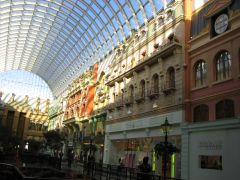
\includegraphics[width=.45\linewidth]{examples/example_1}} \quad
    \subfloat[Pan ma signo.]
    {\label{fig:example-b}%
        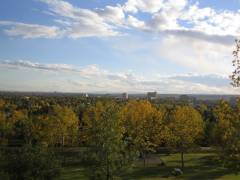
\includegraphics[width=.45\linewidth]{examples/example_2}} \\
    \subfloat[Methodicamente o uno.]
    {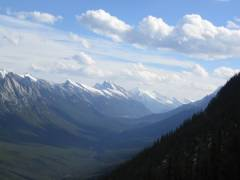
\includegraphics[width=.45\linewidth]{examples/example_3}} \quad
    \subfloat[Titulo debitas.]
    {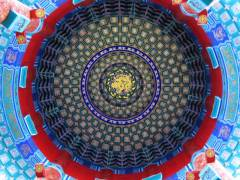
\includegraphics[width=.45\linewidth]{examples/example_4}}
    \caption[Tu duo titulo debitas latente]{Tu duo titulo debitas
        latente. \ac{DRY}}\label{fig:example}
\end{figure}


%*****************************************
%*****************************************
%*****************************************
%*****************************************
%*****************************************

%************************************************
\chapter{Math Test Chapter}\label{ch:mathtest} % $\mathbb{ZNR}$
%************************************************
Ei choro aeterno antiopam mea, labitur bonorum pri no. His no decore
nemore graecis. In eos meis nominavi, liber soluta vim cu. Sea commune
suavitate interpretaris eu, vix eu libris efficiantur.

\section{Some Formulas}
Due to the statistical nature of ionisation energy loss, large
fluctuations can occur in the amount of energy deposited by a particle
traversing an absorber element\footnote{Examples taken from Walter
    Schmidt's great gallery: \\
    \url{http://home.vrweb.de/~was/mathfonts.html}}.  Continuous processes
such as multiple
scattering and energy loss play a relevant role in the longitudinal
and lateral development of electromagnetic and hadronic
showers, and in the case of sampling calorimeters the
measured resolution can be significantly affected by such fluctuations
in their active layers.  The description of ionisation fluctuations is
characterised by the significance parameter $\kappa$, which is
proportional to the ratio of mean energy loss to the maximum allowed
energy transfer in a single collision with an atomic electron:
\graffito{You might get unexpected results using math in chapter or
    section heads. Consider the \texttt{pdfspacing} option.}
\begin{equation}
\kappa =\frac{\xi}{E_{\textrm{max}}} %\mathbb{ZNR}
\end{equation}
$E_{\textrm{max}}$ is the maximum transferable energy in a single
collision with an atomic electron.
\[
E_{\textrm{max}} =\frac{2 m_{\textrm{e}} \beta^2\gamma^2 }{1 +
    2\gamma m_{\textrm{e}}/m_{\textrm{x}} + \left ( m_{\textrm{e}}
    /m_{\textrm{x}}\right)^2}\ ,
\]
where $\gamma = E/m_{\textrm{x}}$, $E$ is energy and
$m_{\textrm{x}}$ the mass of the incident particle,
$\beta^2 = 1 - 1/\gamma^2$ and $m_{\textrm{e}}$ is the electron mass.
$\xi$ comes from the Rutherford scattering cross section
and is defined as:
\begin{eqnarray*} \xi  = \frac{2\pi z^2 e^4 N_{\textrm{Av}} Z \rho
        \delta x}{m_{\textrm{e}} \beta^2 c^2 A} =  153.4 \frac{z^2}{\beta^2}
    \frac{Z}{A}
    \rho \delta x \quad\textrm{keV},
\end{eqnarray*}
where

\begin{tabular}{ll}
    $z$          & charge of the incident particle \\
    $N_{\textrm{Av}}$     & Avogadro's number \\
    $Z$          & atomic number of the material \\
    $A$          & atomic weight of the material \\
    $\rho$       & density \\
    $ \delta x$  & thickness of the material \\
\end{tabular}

$\kappa$ measures the contribution of the collisions with energy
transfer close to $E_{\textrm{max}}$.  For a given absorber, $\kappa$
tends
towards large values if $\delta x$ is large and/or if $\beta$ is
small.  Likewise, $\kappa$ tends towards zero if $\delta x $ is small
and/or if $\beta$ approaches $1$.

The value of $\kappa$ distinguishes two regimes which occur in the
description of ionisation fluctuations:

\begin{enumerate}
    \item A large number of collisions involving the loss of all or most
    of the incident particle energy during the traversal of an absorber.
    
    As the total energy transfer is composed of a multitude of small
    energy losses, we can apply the central limit theorem and describe
    the fluctuations by a Gaussian distribution.  This case is
    applicable to non-relativistic particles and is described by the
    inequality $\kappa > 10 $ (\ie, when the mean energy loss in the
    absorber is greater than the maximum energy transfer in a single
    collision).
    
    \item Particles traversing thin counters and incident electrons under
    any conditions.
    
    The relevant inequalities and distributions are $ 0.01 < \kappa < 10
    $,
    Vavilov distribution, and $\kappa < 0.01 $, Landau distribution.
\end{enumerate}


\section{Various Mathematical Examples}
If $n > 2$, the identity
\[
t[u_1,\dots,u_n] = t\bigl[t[u_1,\dots,u_{n_1}], t[u_2,\dots,u_n]
\bigr]
\]
defines $t[u_1,\dots,u_n]$ recursively, and it can be shown that the
alternative definition
\[
t[u_1,\dots,u_n] = t\bigl[t[u_1,u_2],\dots,t[u_{n-1},u_n]\bigr]
\]
gives the same result.

%*****************************************
%*****************************************
%*****************************************
%*****************************************
%*****************************************
 % Use this as a reference to find out how things are done.

\cleardoublepage\chapter{Introduction}\label{ch:introduction}
 % 3-4 pages
\cleardoublepage\chapter{Related Work}\label{ch:relatedwork}
\section{Large-scale Personal Fabrication}
\section{Construction Kits}
\section{Prototyping with Ready-Made Objects}
\section{Building with Variable Geometry Trusses}
- Steward Platform\\
- Walking Octa\\
\section{Software Pipeline for Animatronics}
\section{SketchUp}
 % 6-8 pages
\cleardoublepage
\chapter{Walkthrough}\label{ch:walkthrough}
\begin{figure}[ht!]
    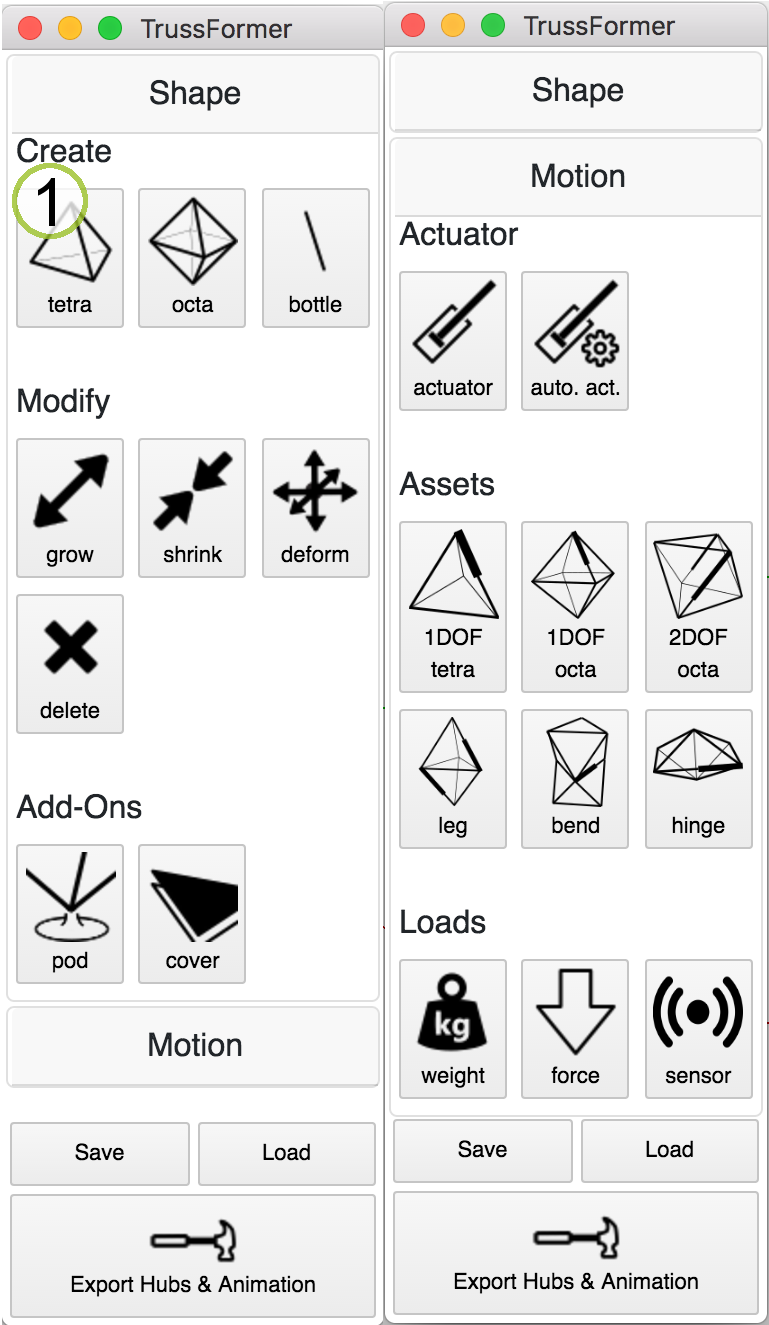
\includegraphics[width=.7\textwidth]{Walkthrough/UI.png}
    \centering
    \caption{TrussFormers' toolbar}
    \label{fig:toolbar}
\end{figure}
This chapter will present the functionalities of the system by showing the process of creating the T-Rex shown in Figure \ref{fig:examples} (c). This will include all steps from creating the static structure, over introducing animation up to fabricating the final object.

\section{Designing Static Structures}
As shown in Figure \ref{fig:modelling_t-rex}, the T-Rex model was first created as a stable static structure. With the help of TrussFormer, the user can make sure that the object to be created is structurally sound before adding motion. The provided tools can create sturdy primitives that are attached to each other, deform the structure, and check forces acting on each part of the object.

\subsection{Primitives}
Users can use predefined and structurally stable primitives to create their objects. Our system provides tools for creating octahedra and tetrahedra (Figure \ref{fig:toolbar} (1)). These truss primitives consist entirely of triangular faces, which is an essential property for stable objects and widely used in heavy industry and architecture, e.g. cranes or bridges.

\subsection{How they are used}
The primitives can be attached to existing triangle faces, as seen in Figure \ref{fig:modelling_t-rex} or placed on the ground. If necessary, our system can also create single links between two nodes using the bottle link tool (2).\\
The form of the structure can be tweaked as desired by using the grow and shrink tool (3). These tools elongate or shorten edges, deforming the structure in such a way that the truss structure stays intact. As our PET bottle system only allows three different sizes of edges (two big bottles, one big and one small bottle, two short bottles), we elongate the connecting parts on the nodes. The grow and shrink tools will change the length of the \textit{elongation} as long as a different bottle configuration is possible. So, if the users wants to shorten a certain edge a lot, the shrink tool will determine, that it should become a short-short bottle link and adapt the elongations accordingly. The deform tool (4) does a similar job, but rather than working on edges, this tool can move nodes.\\
For settling the object on the ground or placing a cover on a triangle face, TrussFormer also provides a pod tool (5). Pods provide a flat surface on nodes that stands proud of the curved bottle bodies, making it easier to have a firm and level stand. Nodes that have a pod will not be changed by the modifying tools.

\begin{figure}[ht!]
    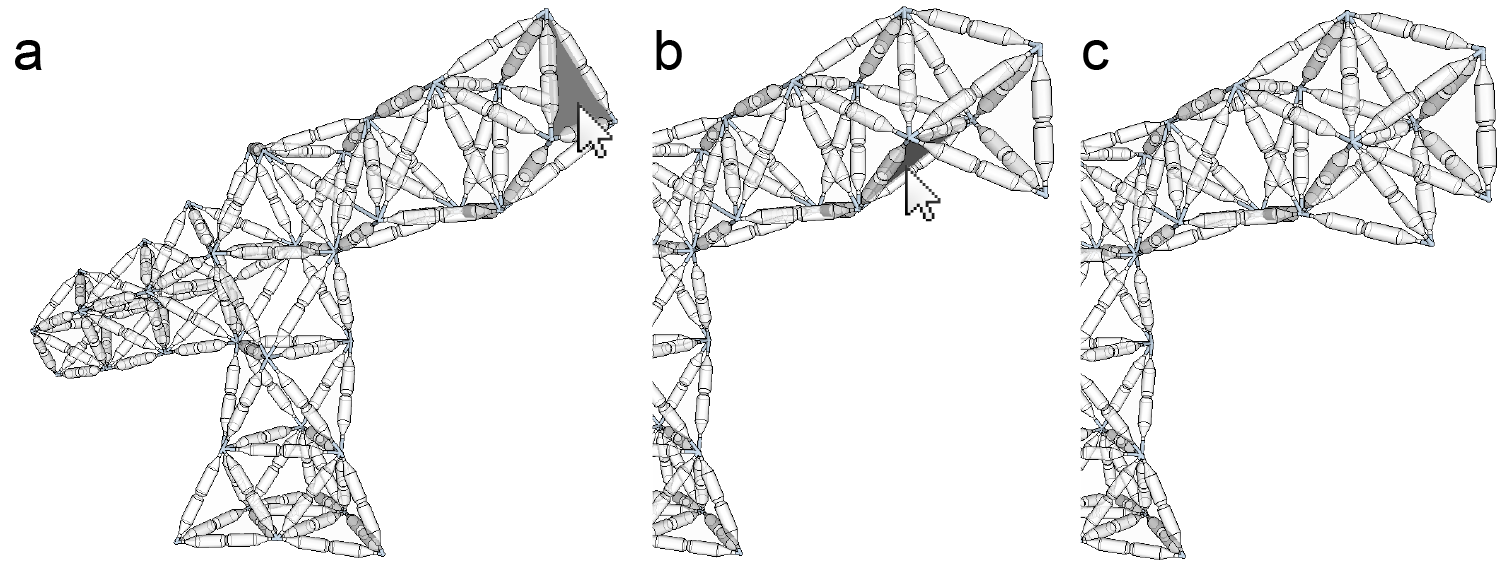
\includegraphics[width=\textwidth]{Walkthrough/modeling_dino_(trussfab)-01.png}
    \centering
    \caption{Modeling the static shape of the T-Rex. Here, the user creates the jaws of the T-Rex by attaching tetrahedron primitives through the steps (a, b, c).}
    \label{fig:modelling_t-rex}
\end{figure}

\subsection{Check static forces}
Using the animation pane, the user can determine static forces acting on the structure. TrussFormer provides tools for adding weight to the structure. In the case of our T-Rex, users might want to add decoration with a weight of 5 kg to its head. The select the \textit{Add Weight Tool} (6) and select a node. After that, they click the \textit{Play} (Figure \ref{fig:animation} (12)) button in the animation window. Our built-in simulation will visualize occurring forces and check if the structure is capable of withstanding the additional force.

\section{Adding Movement to the Structures}
Movement is added to the structure by placing special physics links. These links act like linear actuators - struts that can extend and retract in a straight line. There are multiple methods for placing these actuators, ranging from a fully-automated way to manual placement.

\subsection{Automatic Actuator Placement}
The automated way works by demonstrating a desired movement. The user selects the \textit{Demonstrate Movement Tool} (6), clicks a node that should experience a certain movement and drags a line to the desired end position. TrussFormer will then search for an actuator that brings the node closest to the desired position and turns the resulting edge into an actuator. The tool runs through all edges of the structure, replacing one after another with an actuator and simulates the resulting movement in the background. The actuator that solves the problem the best will be placed.
\begin{figure}[ht!]
    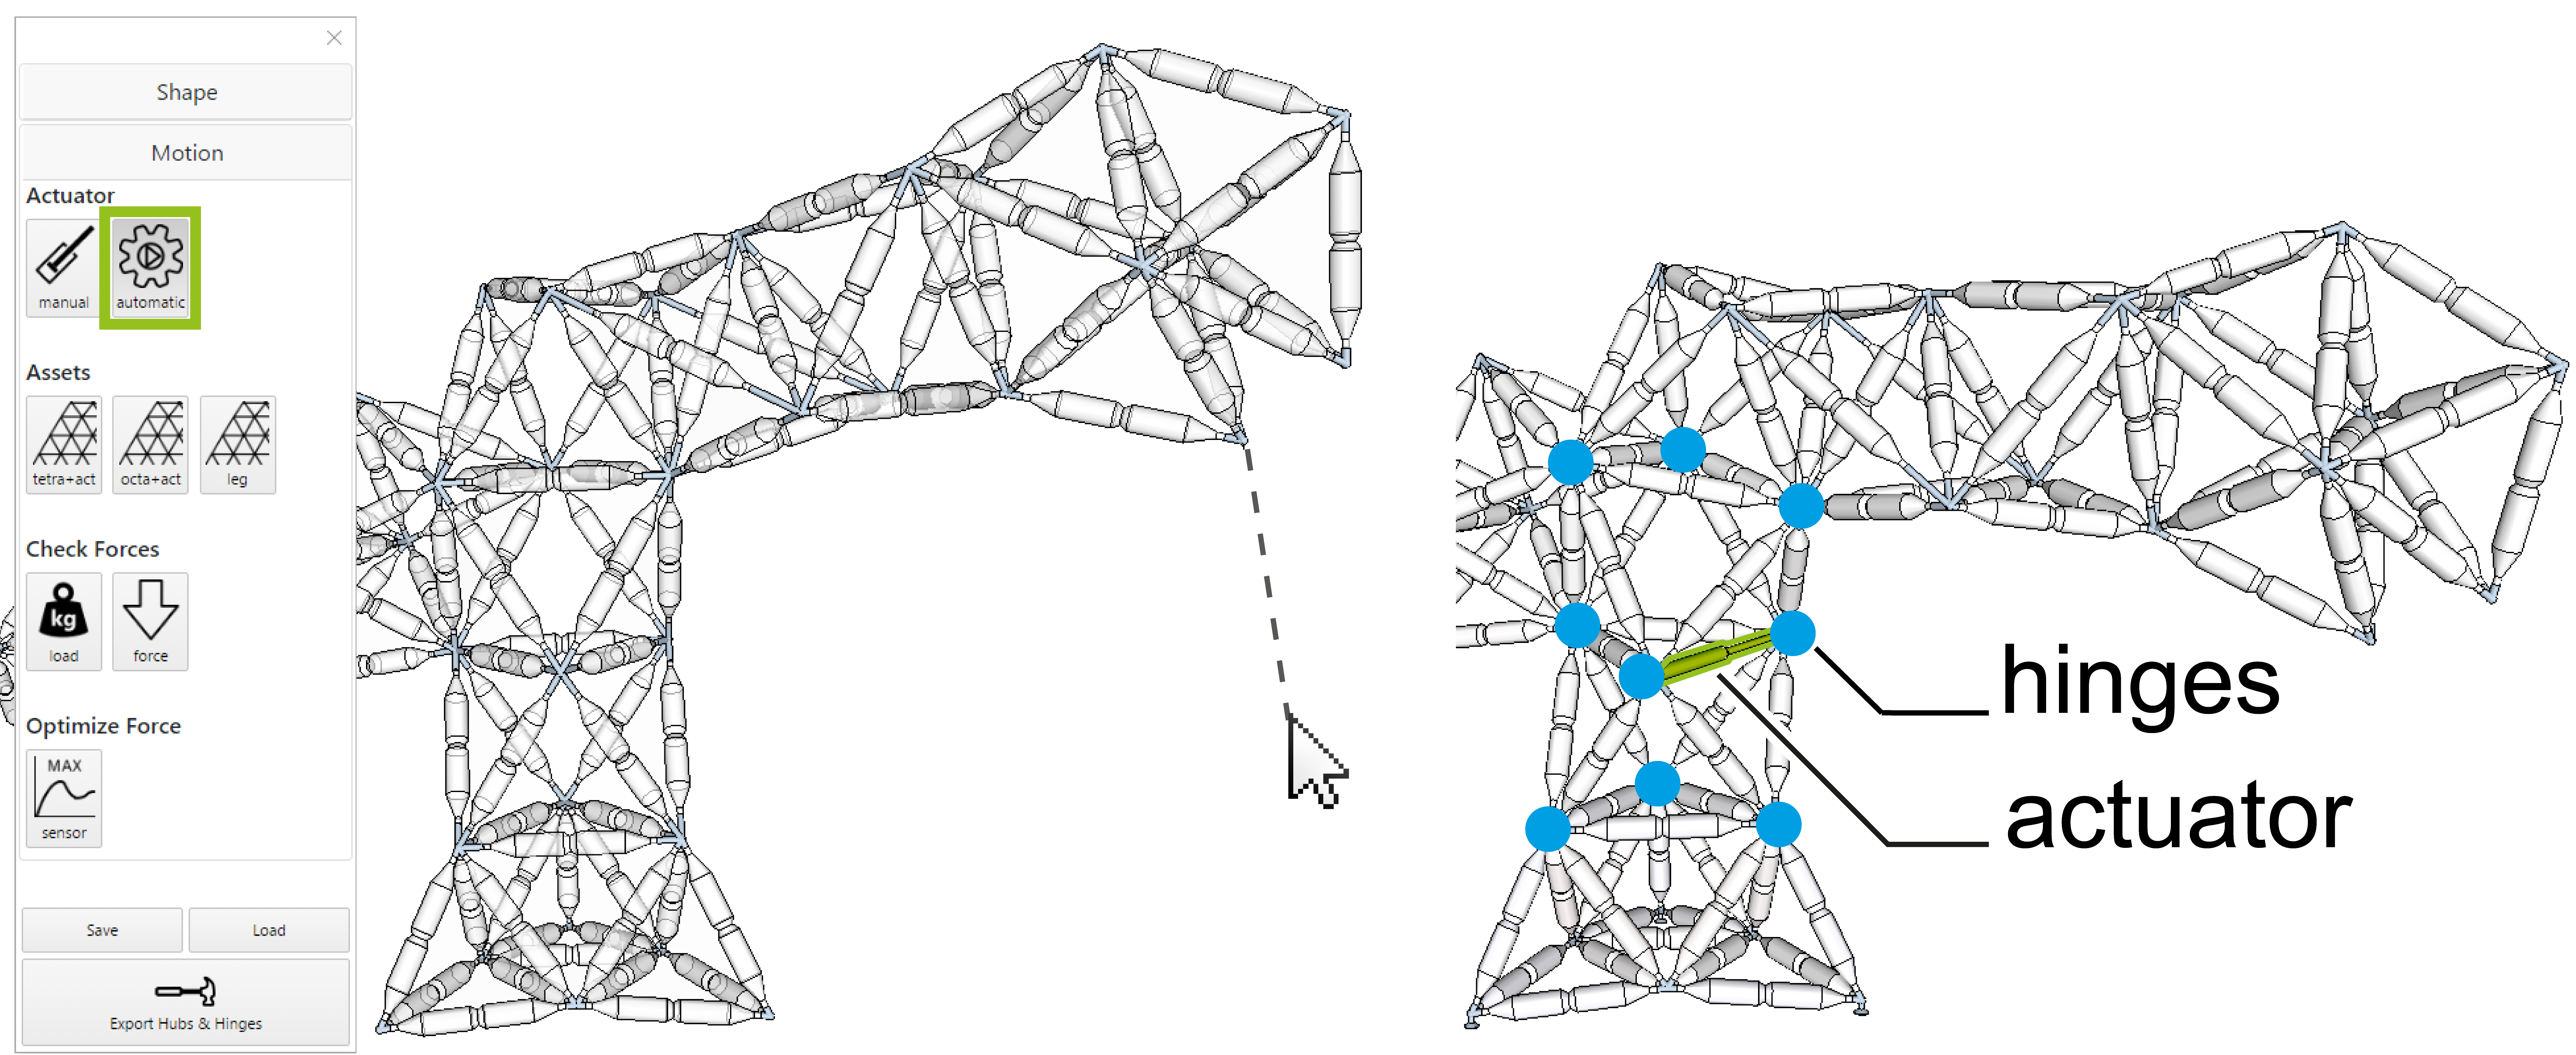
\includegraphics[width=\textwidth]{Walkthrough/demonstrate_movement_tool.png}
    \centering
    \caption{(a) The user selects the demonstrate movement tool and pulls the T-Rex head downwards. (b) TrussFormer responds by adding an actuator to the T-Rex body so that it is capable of performing this type of motion. At this point the system also places 9 hinging hubs to enable this motion (marked with blue dots).}
    \label{fig:demonstrate_movement}
\end{figure}

\subsection{Placing Primitives}
Another way to add movement is to use predefined dynamic assets. It can be difficult for a user to fully grasp how an actuator will move the whole object. We encapsulated often-used assets into tools (7). These assets connect to the rest of the structure through a dedicated triangle surface. Because the motion is localized in this asset, the result in the bigger structure is easier understandable. A selection of assets is shown in Figure \ref{fig:dynamic_assets}\\
Instead of using the demonstrate movement tool to create the nodding motion of the T-Rex, a ``bending'' double-octahedron, as seen in Figure \ref{fig:dynamic_assets} (f) could have been used in the vertical body part.
\begin{figure}[ht!]
    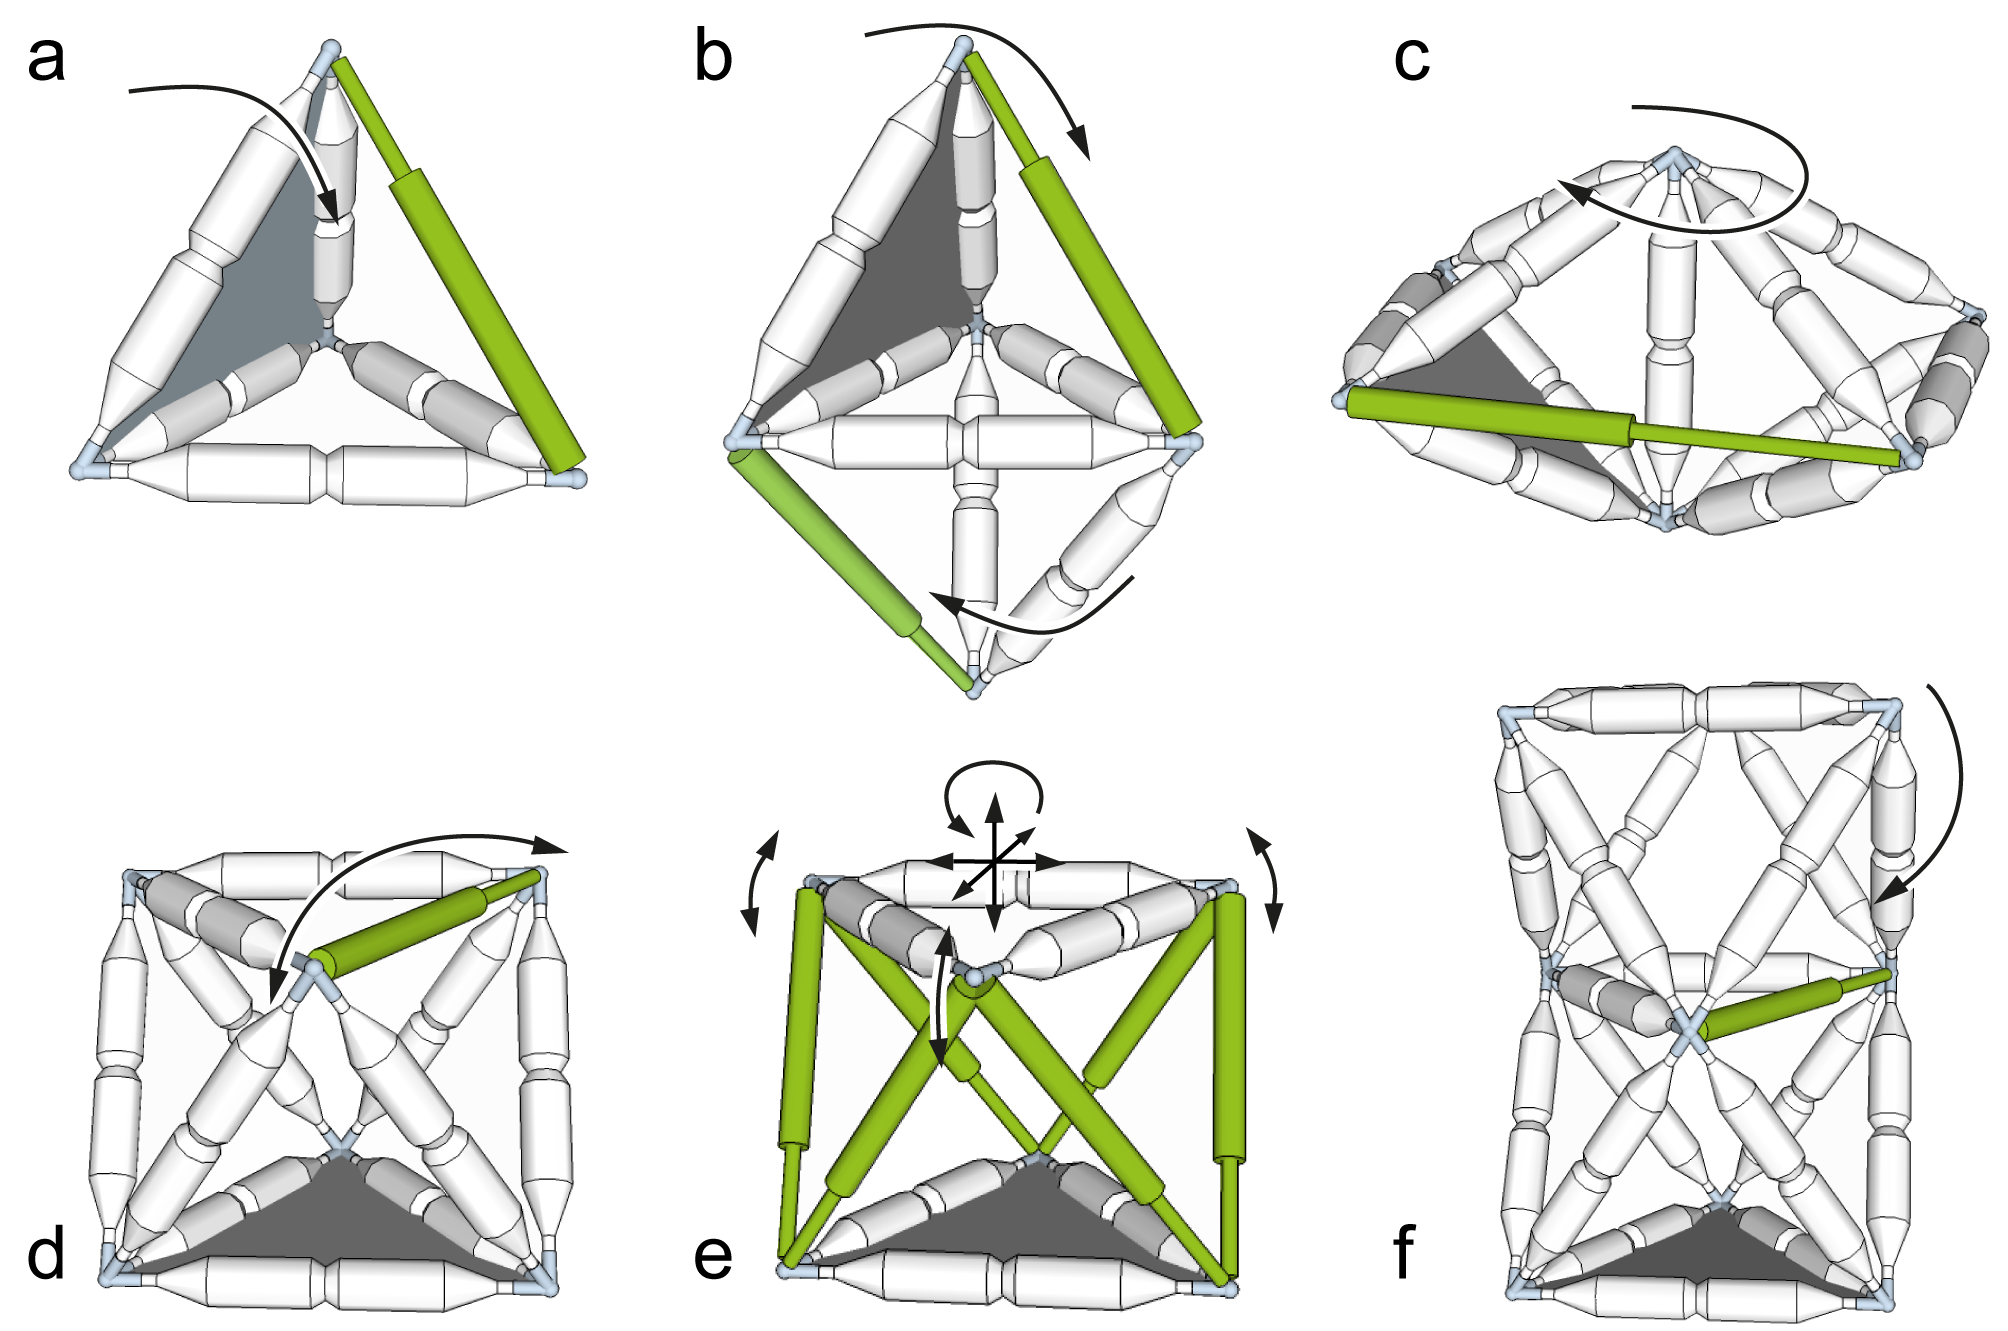
\includegraphics[width=\textwidth]{Walkthrough/assets_white-01.png}
    \centering
    \caption{A selection of assets: (a) tetrahedron with 1DoF, (b) “robotic leg” asset, (c) hinging tetrahedra, (d) octahedron with 1DoF, (e) Stewart platform (6DoF), and (f) double-octahedron performing “bending” motion.}
    \label{fig:dynamic_assets}
\end{figure}

\subsection{Manual Actuator Placement}
The manual actuator placement requires the most knowledge about the resulting motion. It is, however, the most flexible way to create movement. The user can choose the \textit{actuator tool} (8) to turn any edge into or connect two nodes with an actuator. This can be done by clicking on the desired edge or selecting two nodes to be connected. Transforming an existing edge is usually the desired use case, as the introduction of more edges (by connecting two previously unconnected nodes) tends to make the truss more stable and can prevent motion altogether. Turning an edge into an actuator essentially removes this edge and adds a degree of freedom.
\begin{figure}[ht!]
    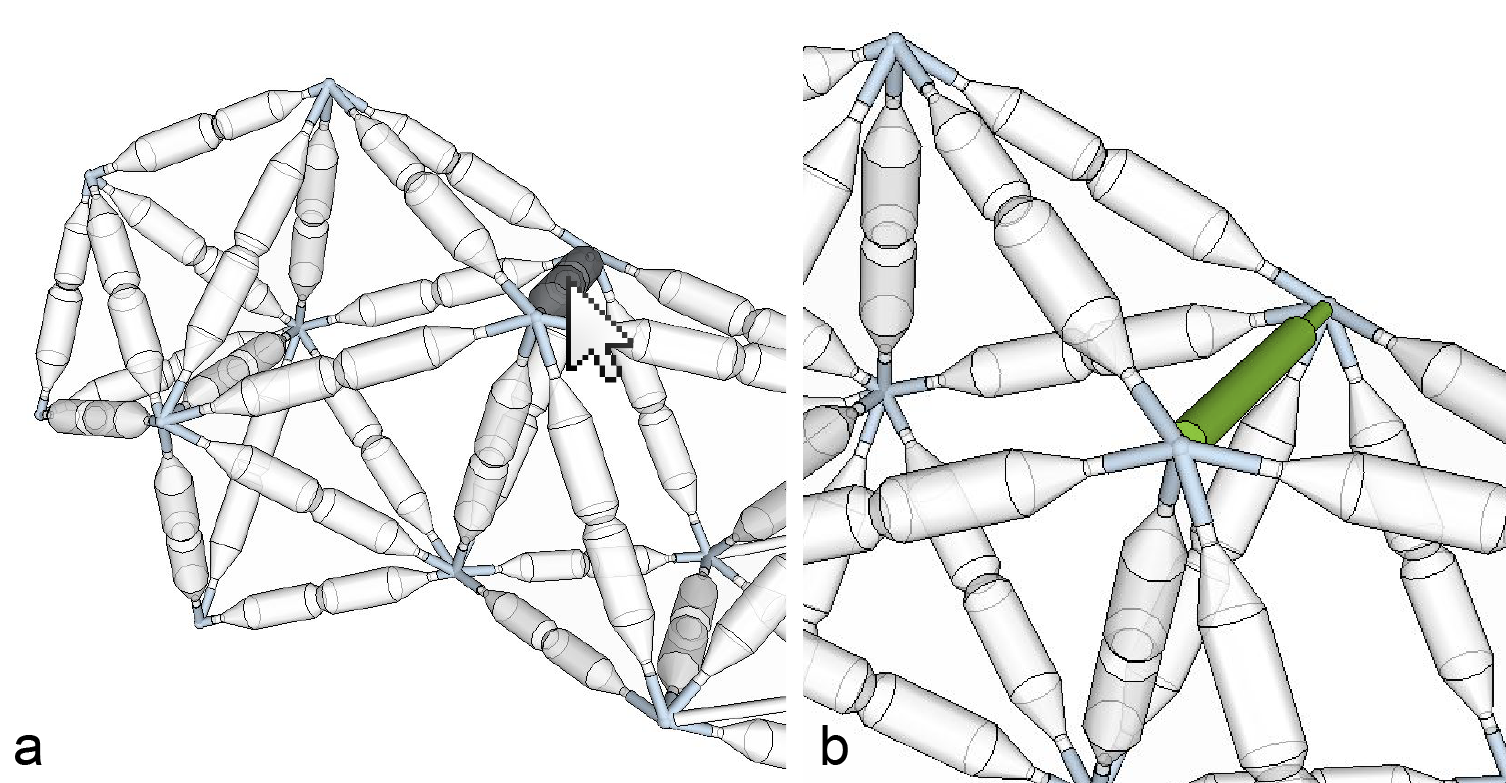
\includegraphics[width=\textwidth]{Walkthrough/manual_actuator_placement.png}
    \centering
    \caption{The turn edge to actuator tool allows users to turn any edge into an actuator. Here user replaces one edge in the T-Rex’s head to make its jaws move.}
    \label{fig:manual_actuator}
\end{figure}

\subsection{Stability Check}
During the placement of actuators, TrussFormer verifies that the mechanism is structurally sound. The system finds the safe range of actuation in the background, i.e. how far an actuator can extend without damaging the structure, by simulating the occurring forces in a range of positions. Damage can occur if the structure falls over, hits the ground with too much speed or if too much force is exerted on a structural element, such as an edge, as illustrated in Figure \ref{fig:check_poses}. To do this, TrussFormer iteratively extends each actuator and observes the forces. If the force exceeds a preset limit, the last safe actuation range is stored in the actuator. The user will then not be able to over-actuate this actuator.\\
To completely prevent breaking, this process would have to be done for each combination of actuators. As this does not scale well with an increasing number of actuators in the system, we perform this step for each actuator individually. An additional security check is done while the user tries out the motion manually, as explained in the next section.
\begin{figure}[ht!]
    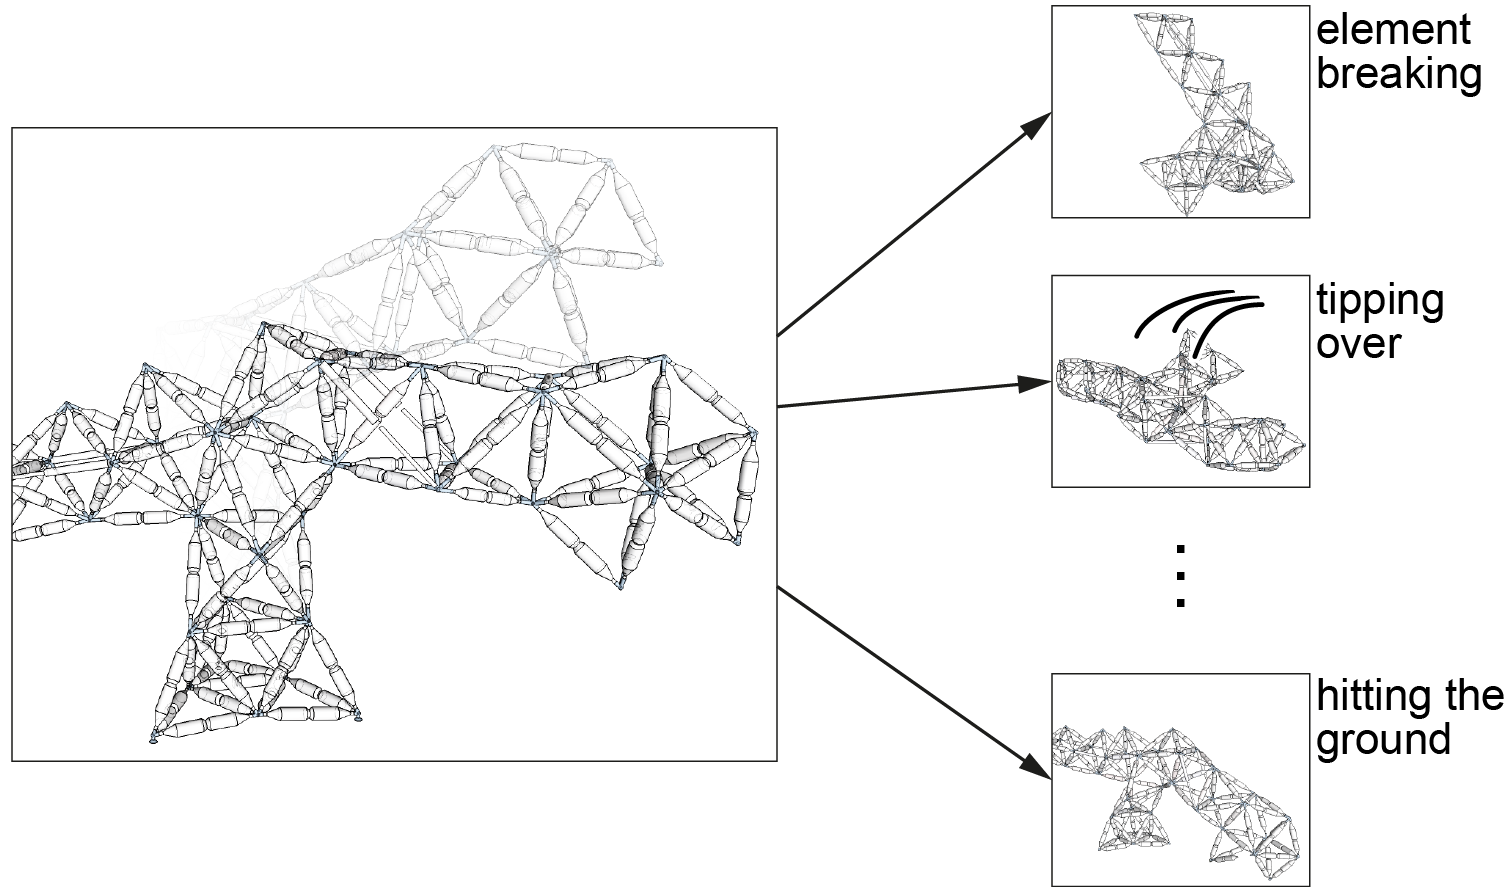
\includegraphics[width=\textwidth]{Walkthrough/check_poses.png}
    \centering
    \caption{In the background, TrussFormer tests each actuator to see if its extension leads to invalid configurations, such as the structure falling over, hitting the ground, or encountering broken structural elements.}
    \label{fig:check_poses}
\end{figure}

\section{Animation}\label{sec:animation}
The user can actuate the physics links in two different ways. The \textit{animation window} provides a slider for manual movement Figure \ref{fig:animation} (9), as well as an animation pane which allows placing keyframes (10) and provides two playback modes (11). All actuators have an actuator group assigned to them. Per default, an actuator is placed in its own, empty group. Using the actuator tool (Figure \ref{fig:toolbar} (8), already used for placing actuators, this group can be changed. This is indicated by the actuator changing its color.\\
The control elements of the animation window always work on the whole group. The color of the animation line indicates which group will be actuated by either the slider or the keyframes.
\begin{figure}[ht!]
    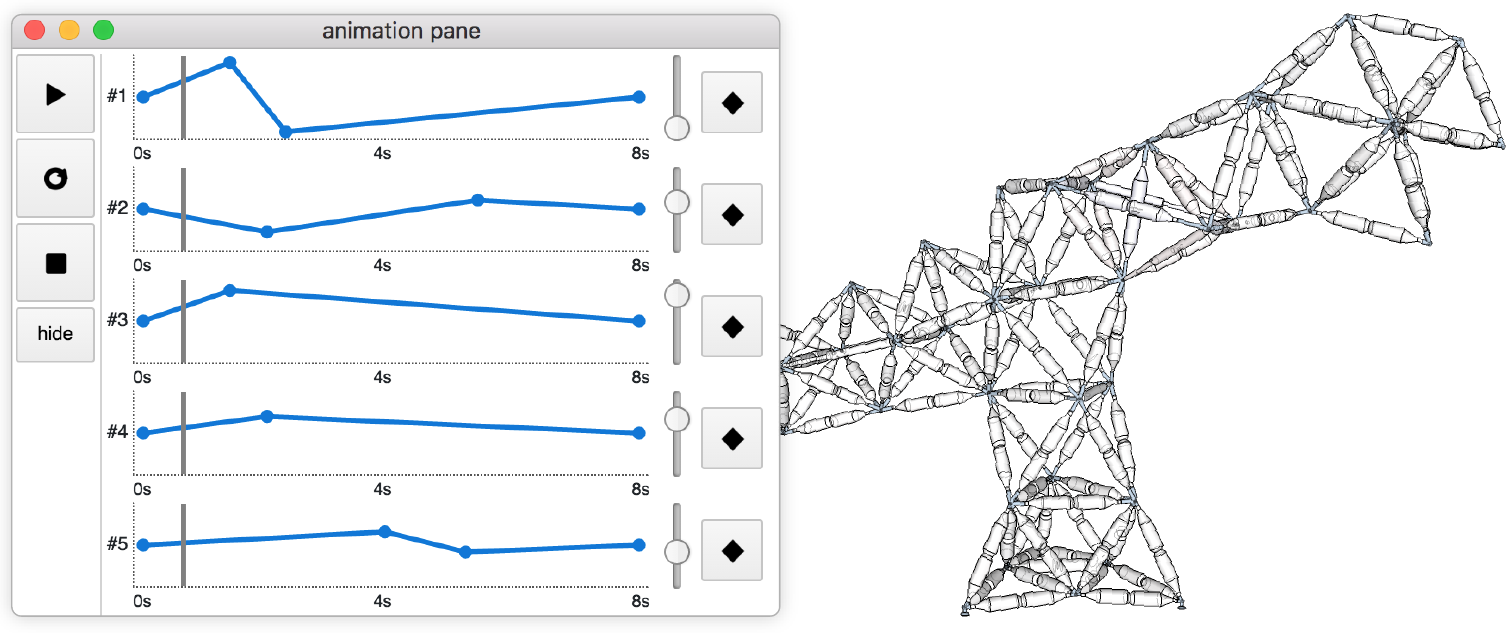
\includegraphics[width=\textwidth]{Walkthrough/animating_the_structure.png}
    \centering
    \caption{Animating the structure. Users sets the desired pose using the sliders in the animation pane and orchestrate the movement by placing key-frames on the timeline. Each timeline controls actuators with the same color.}
    \label{fig:animation}
\end{figure}
To add a keyframe to the animation pane, first the slider has to be moved to the desired position. The object will start to move according to the sliders position - if the slider is at the top, the actuator will be fully extended and vice versa. That way, the user can visualize the extend of the movement. If the user is satisfied, the indicator line can be moved to the desired position in the timeline and the diamond button is pressed to add this keyframe to the animation.

\subsection{Checking Dynamic Forces}
If the structure fulfills the desired motion, the user will want to check if the forces created during executing it will not exceed the breaking force of the object. A lot of factors play a role in the formation of forces. These range from weight forces over lever forces to inertial forces. TrussFormer aids the user to detect weak points and force peaks during a motion in different ways.\\
TrussFormer's tools provide the possibility to constantly monitor the forces that occur during interactive movement of the structure. In simulation mode, all edges will be colored red or blue in increasing intensity the higher the force on them is. Red indicates compression force, while blue means tension force. A completely white color indicates a force of $0 N$. These tension forces are automatically calculated by the built-in physics engine.\\
As shown in Figure \ref{fig:fix_breaking} (a) the user creates an animation that moves the T-Rex body down and up again. (b) While TrussFormer plays the animation, it calculates the forces. The change from the downwards motion to going up again causes a lot of contraction force on the edges on the front body side. The neck of the T-Rex acts as a lever, which leads to very high inertial forces. This motion eventually exceeds the breaking limit of the structure, (c) causing the construction to fail. The time of breaking is indicated in the animation pane by a red vertical line. This failure is hard to predict by the user, because inertial forces can be multiple times higher than the static forces, checked during the creation of the T-Rex. (d) TrussFormer helps the user to fix the motion. A popup is opened providing two possibilities (Figure \ref{fig:correcting_animation}): fixing the animation by reducing the speed or reducing the motion. If the first option is chosen, TrussFormer will elongate the animation sequence for all piston groups. This results in a slower movement and less force on the structure. The second option will keep the length of the animation, but move the keyframes closer to the center line. The amplitude of the motion will be decreased this way.\\
Both versions will reduce the acceleration of the structure. The force formula $F = m * a$ shows, that the force increases proportionally with the acceleration, as the mass is constant in the structure. Reducing acceleration also reduces the force.
\begin{figure}[ht!]
    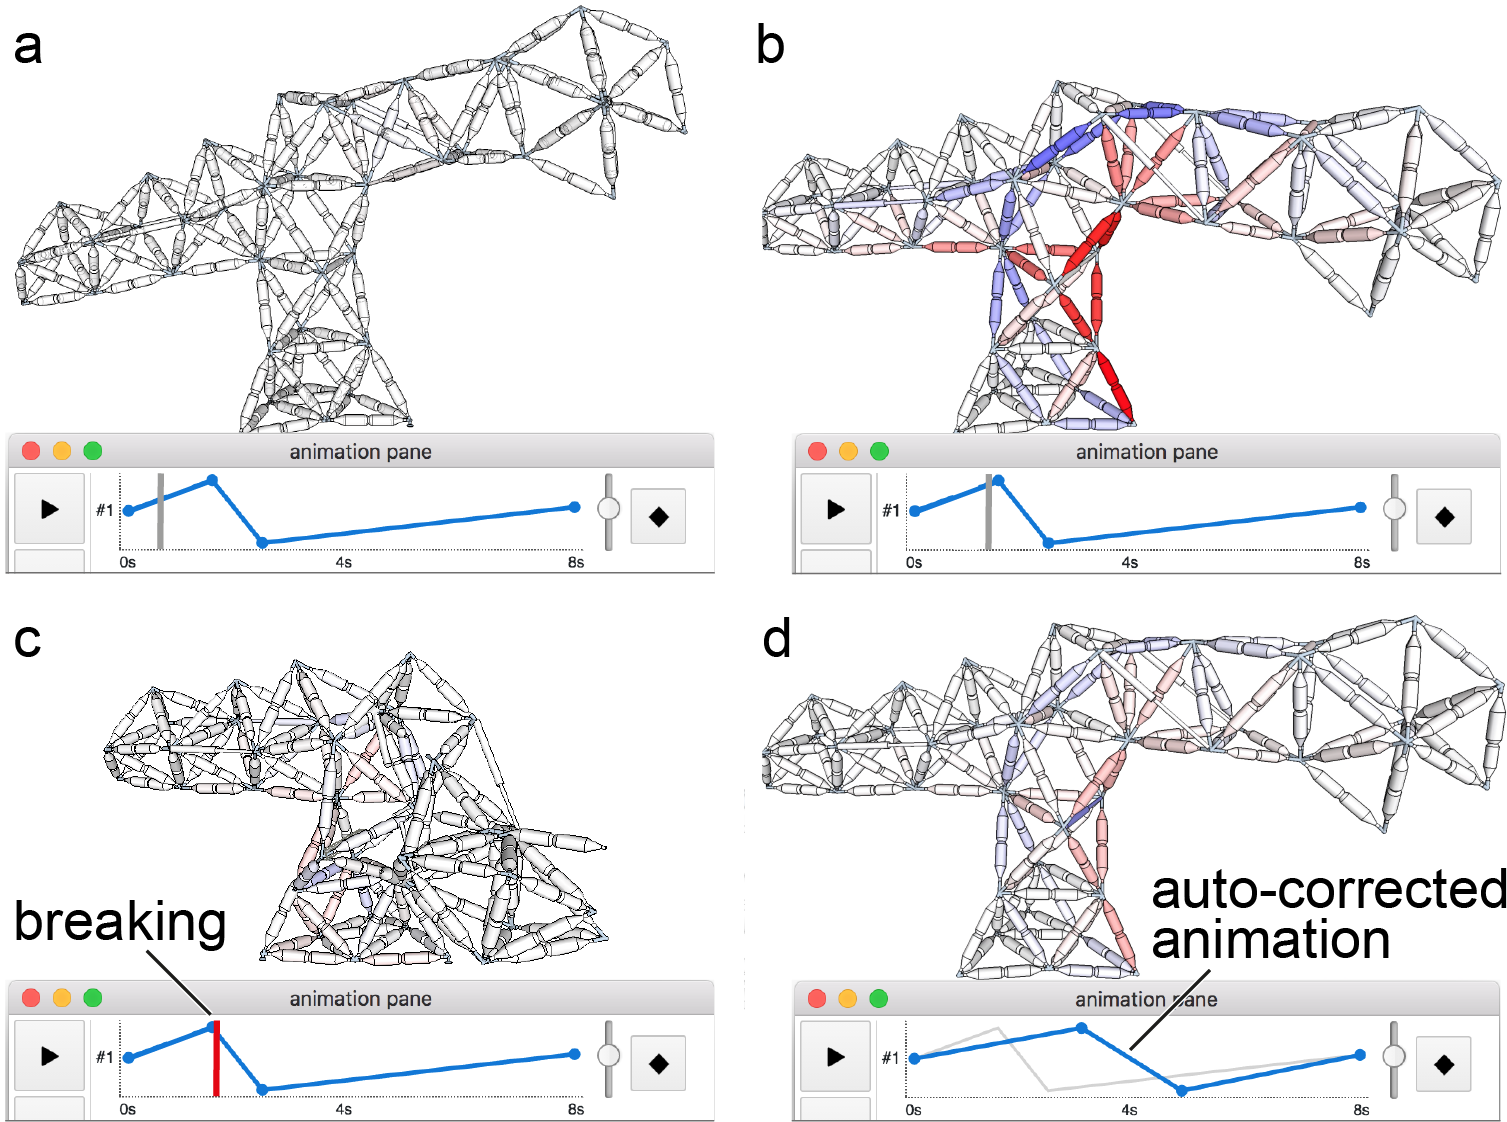
\includegraphics[width=\textwidth]{Walkthrough/forces-01.png}
    \centering
    \caption{TrussFormer verifies that the structure can withstand the inertial forces resulting from the programmed animation. (a-b) The forces in the T-Rex increase with the movement. (c) The structure breaks when the direction of the movement changes rapidly. (d) TrussFormer resolves this by making the movement slower.}
    \label{fig:fix_breaking}
\end{figure}
\begin{figure}[ht!]
    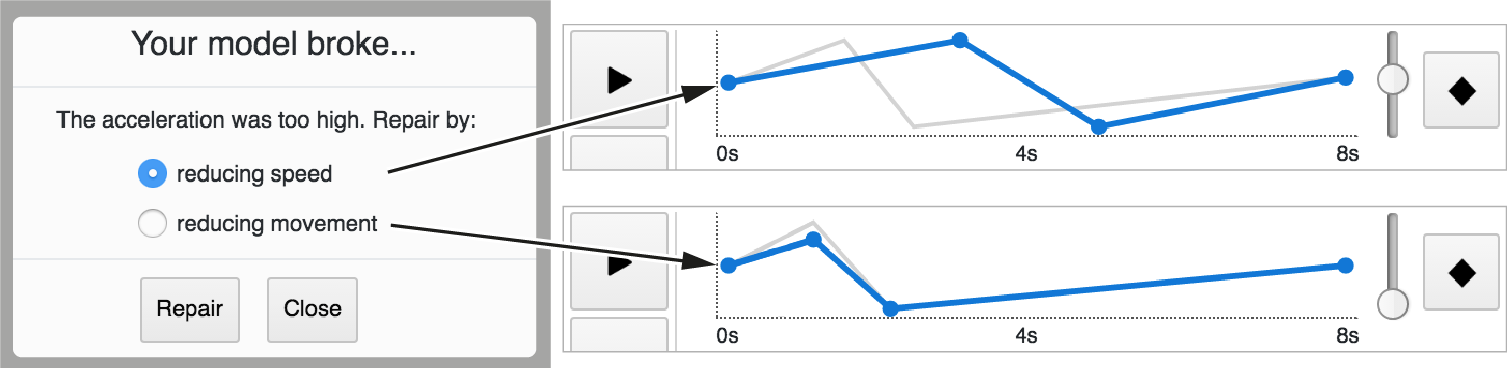
\includegraphics[width=\textwidth]{Walkthrough/auto_correcting_animations.png}
    \centering
    \caption{If the user-defined animation breaks the model, TrussFormer offers to automatically reduce the speed or the motion range.}
    \label{fig:correcting_animation}
\end{figure}

On top of the coloring of edges, the user can also use the \textit{sensor tool} (12). This tool can be used on a single edge to observe it more closely. The force data on an edge with a sensor will be recorded and visualized over time in a chart. The sensor tool also works on nodes, visualizing speed and acceleration data, instead of force. The result can be seen in figure \ref{fig:sensor}.\\
\begin{figure}[ht!]
    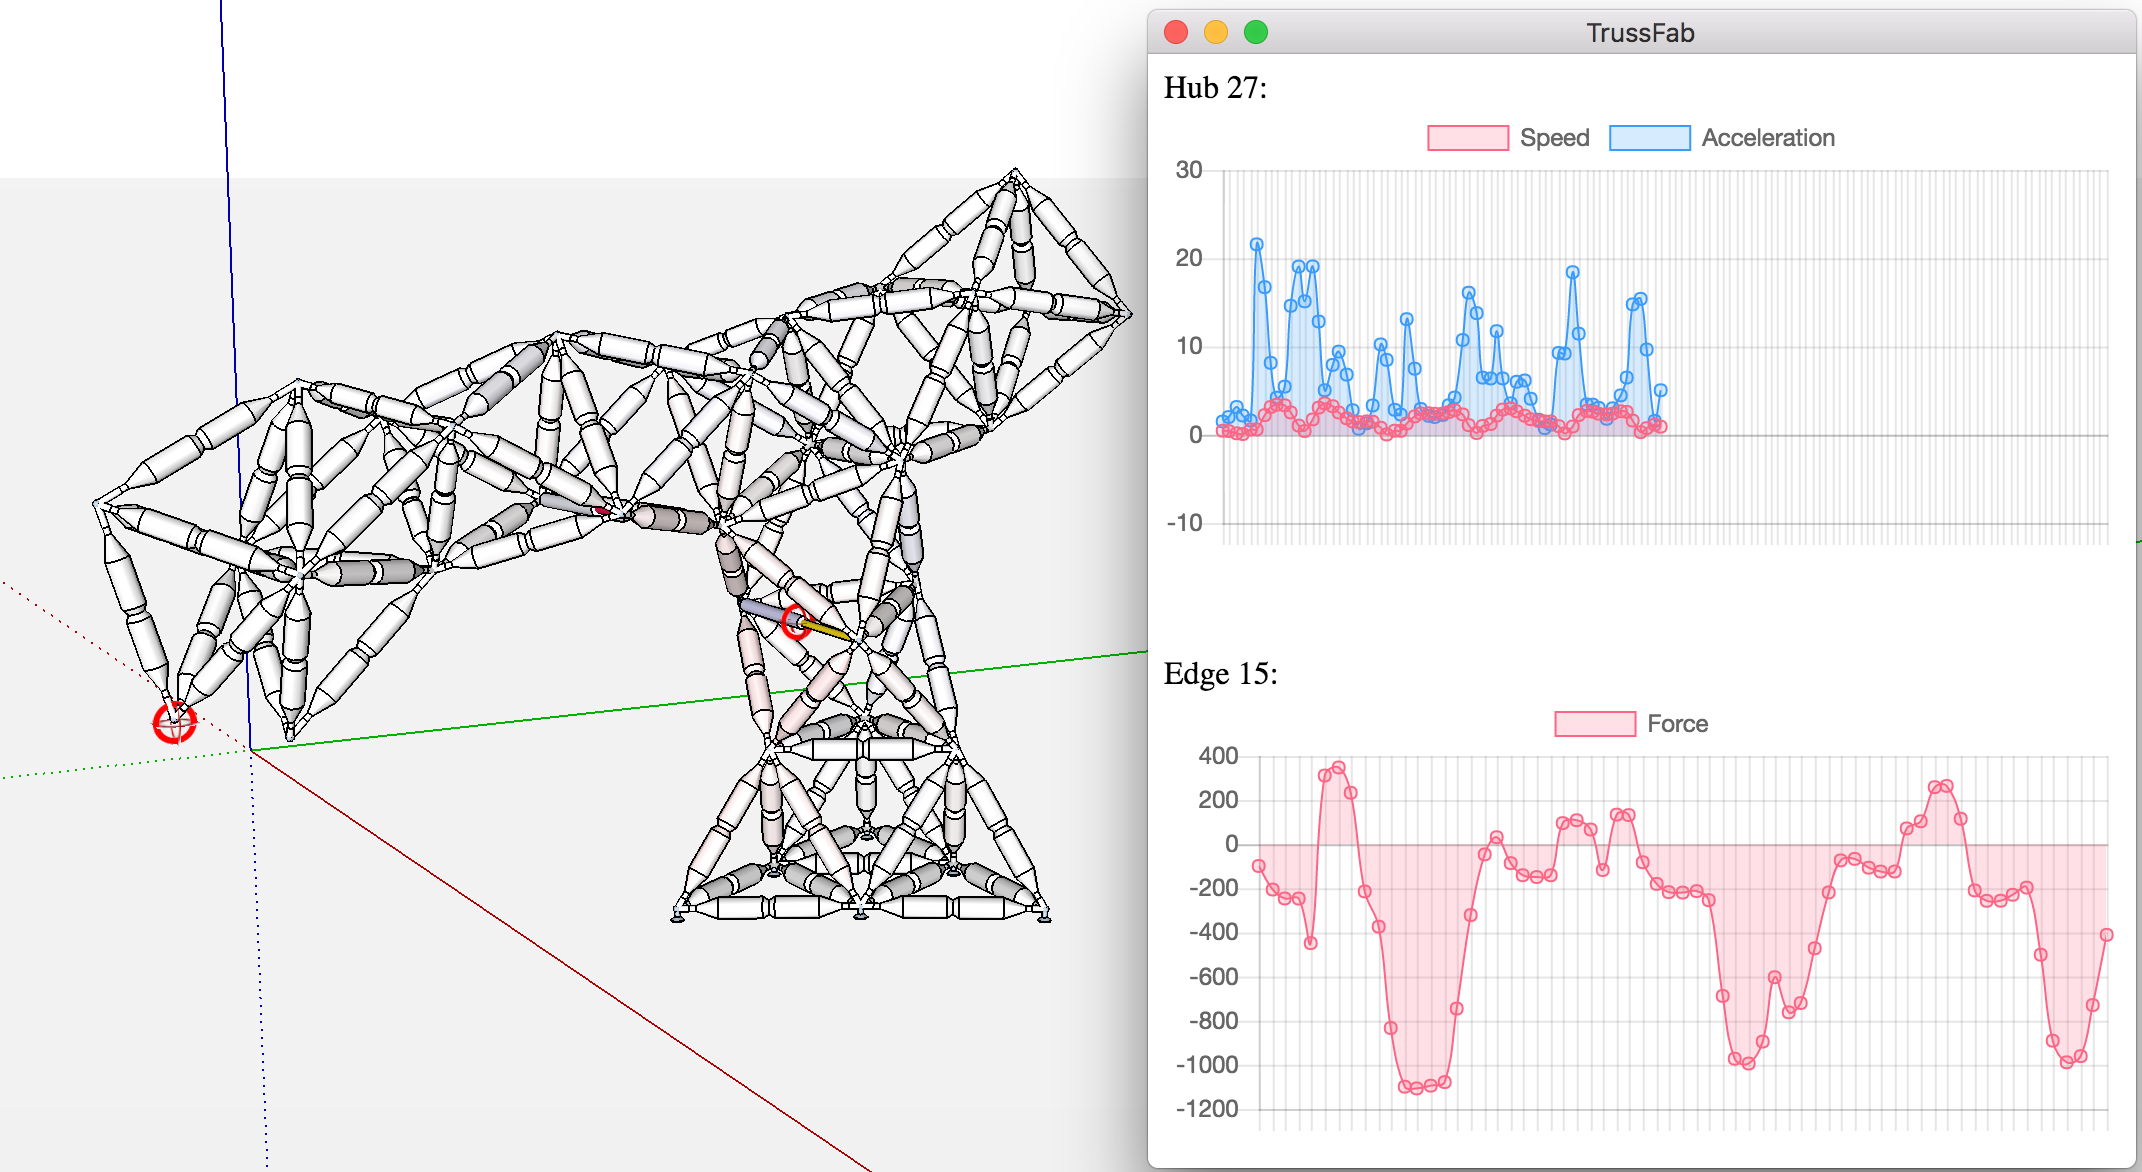
\includegraphics[width=\textwidth]{Walkthrough/sensor.png}
    \centering
    \caption{A sensor measures the force on the central actuator, and speed and acceleration on a node at the ``nose'' of the T-Rex}
    \label{fig:sensor}
\end{figure}

\section{Fabrication}
After the object was sufficiently tested in the editor, users want to print the connectors and assemble the final object. To do this, TrussFormer will calculate which connections need to move in the printed object and which can be static. It also takes into account constraints, such as the minimum distance from a bottle neck to the center of a hinge, which might otherwise restrict movement. This process will be explained in detail in Section \ref{sec:hinge_placement_impl}.

\subsection{Export}
When users are satisfied with their design (structure, movement, and animation), they click the \textit{fabricate} button (13). This will trigger TrussFormers' hinge generation procedure and create files which can be used for 3D printing. In order to control the structure the same way as in the animation pane, the animation will also be exported in an Arduino-readable format. Instructions for building will also be provided.
\begin{figure}[ht!]
    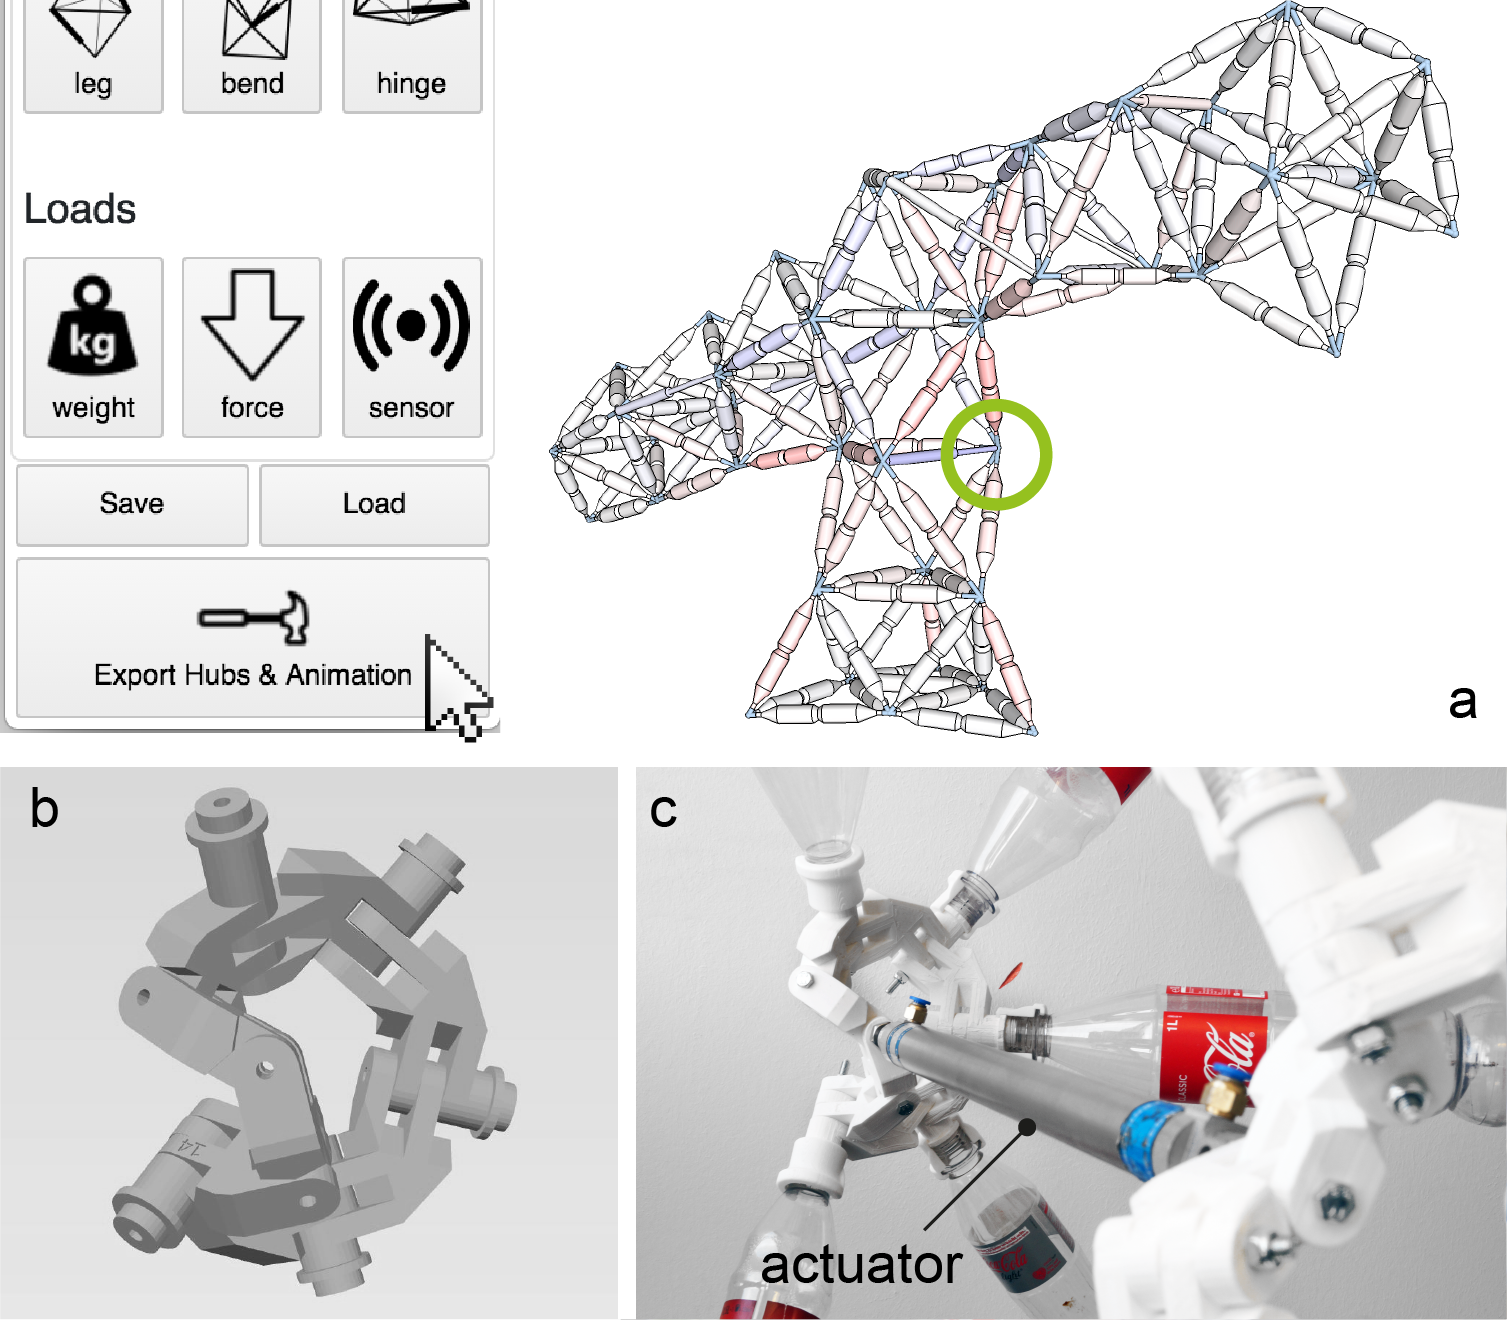
\includegraphics[width=\textwidth]{Walkthrough/export_and_hinges.png}
    \centering
    \caption{(a) To fabricate our T-Rex model, TrussFormer exports: (b) the appropriate 3D printable hinging-hubs for fabricating the structure, (c) and the actuator specifications that inform the users which one to buy. TrussFormer also exports the animation sequence for an Arduino.}
    \label{fig:export_and_hinges}
\end{figure}

TrussFormers' hinge generation procedure will analyze the structure, ensuring that the final object has the maximum possible movement and creates 3D printable hinge and hub geometries. The T-Rex consists of 42 3D printed hubs and 135 unique hinge pieces.\\
Next, the animation pattern is exported to Arduino code. The user can upload this code directly to their microcontroller.\\
As a last step, specifications containing information about the force, speed and motion range of the actuators necessary for achieving the desired animation pattern, are created. Actuators that fulfill these requirements can be obtained as standardized components. The specifications also include information about the number and size of screws needed for assembly.

\subsection{Printing the Parts}
Each exported file represents a single part in the structure. These files can easily be converted to \textit{.stl} files, which are typically used for 3D printing. Using a 3D printing software, the 3D objects can be arranged and sent to a 3D printer. Printing of one hinge part using an UltiMaker 3 printer takes about 40 minutes.

\subsection{Assembling the Structure}
The resulting hubs and hinges contain an ID system for easy assembly. Each part of a node has the node ID printed on. That way it is easy to find out which hinge-parts belong together. Additionally, each edge elongation contains the id of the connected edge. Two hinge parts with the same node ID and edge ID will be connected.\\
Two connectors with different node IDs but the same edge IDs will be connected by an edge.
\begin{figure}[ht!]
    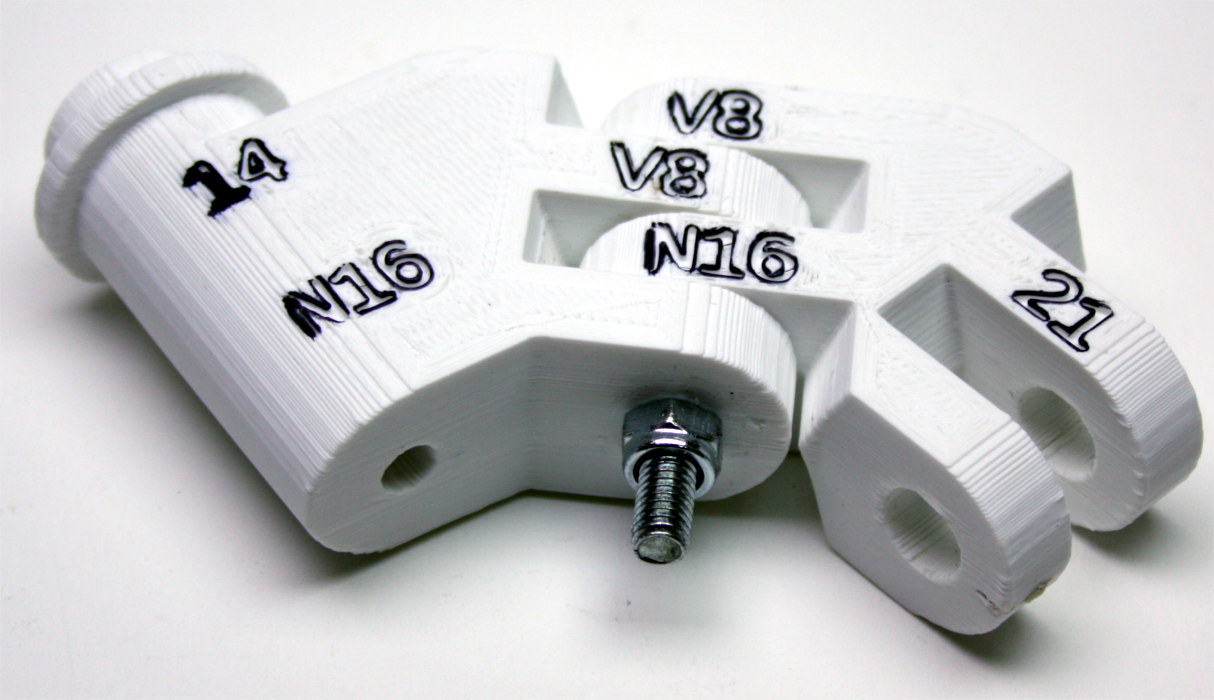
\includegraphics[width=\textwidth]{Walkthrough/hinge.png}
    \centering
    \caption{Two hinge parts connected. Both belong to Node 14 (N14) and their connection has the ID V8, indicating that this is an intermediate hinge connection (explained in Section \ref{sec:hinges}). The left connector will be linked by Edge 14.}
    \label{fig:hinge}
\end{figure}
 % 5-8 pages
\cleardoublepage\chapter{Hardware}\label{ch:hardware}
The system presented in this paper makes use of a variety of mechanical components. This chapter will talk about mechanical challenges and our solutions that allow the construction of large-scale dynamic truss objects using 3D printed parts. It will explain the materials and methods used in creating a real-world object from a TrussFormer-designed model.\\
Furthermore, this chapter will define the techniques and hardware employed in the structures.

\section{Mechanical Components}
We can differentiate between three essential building parts for our truss objects. We call the structural components \textit{links}. In our objects PET bottles are used as links, as they are readily available, cheap and sturdy.\\
We have two different ways of connecting links. Rigid connections are comprised of \textit{static hubs}. For dynamic connections, i.e. connections that allow movement of the structure, we use \textit{hinging hubs}.\\
Links, and static or hinging hubs are connected by purpose-designed \textit{cuffs}, which fit over the bottle's thread on one side and a connector part on the hub on the other side, as seen in Figure \ref{fig:connector} (b).

\subsection{Edges of the structure}
We opted to use 1l (big) and 0.5l (small) reusable PET bottles because they have thicker walls, providing more stability and are abundantly available. Two bottles are connected on their bottom side by a wood screw, which is inserted using a special long-necked screwdriver. This process is depicted in Figure \ref{fig:connect_bottles}. The resulting link-lengths are:
\begin{enumerate}
\item 60 cm - two big bottles
\item 53 cm - one big and one small bottle
\item 46 cm - two small bottles
\end{enumerate}

\begin{figure}[ht!]
    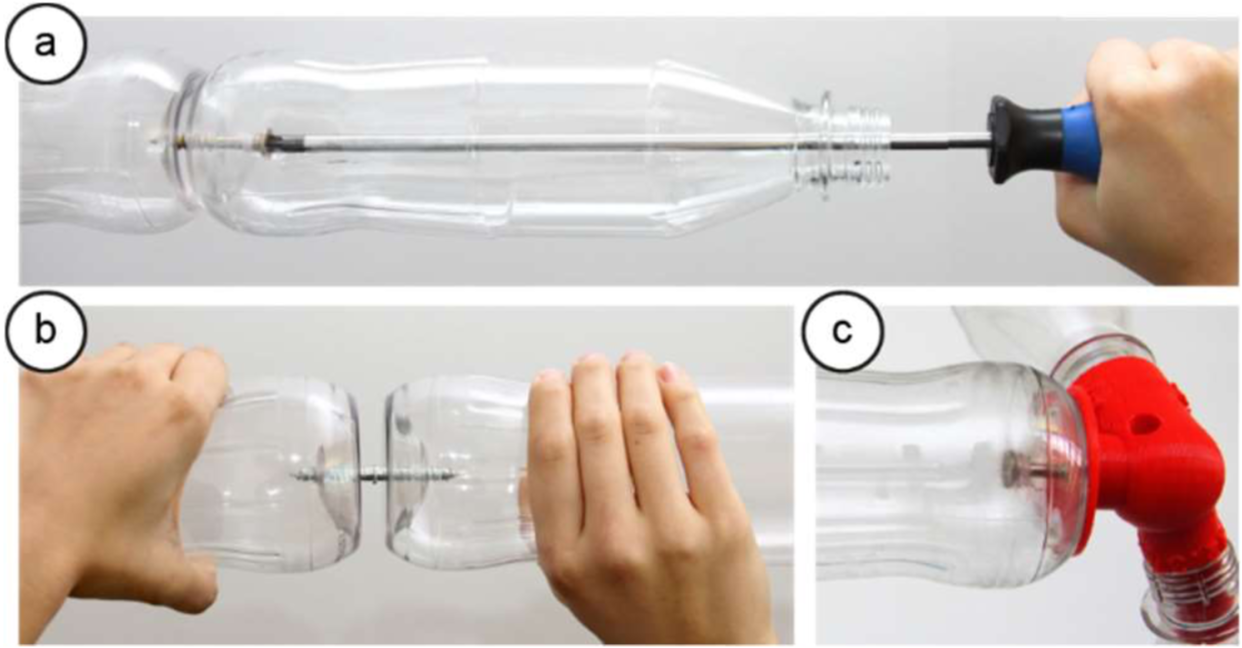
\includegraphics[width=\textwidth]{Hardware/connect_bottles.png}
    \centering
    \caption{(a) Connecting bottles with a wood screw using an extra-long screwdriver and (b) with a double-ended screw. (c) Single-bottle edges require a bottom connector}
    \label{fig:connect_bottles}
\end{figure}

\subsection{Rigid hubs}
We call the connecting parts \textit{hubs}. These hubs are designed to withstand loads in the range of a human weight. Earlier tests show, that the bottle links we use can withstand a compression force of around 85 kg.\\
Hubs are solid one-piece objects that can connect two or more links. They therefore have two or more regions that can hold the neck of a bottle. We call these regions \textit{connectors}. These connectors consist of a flat part, slightly wider (30 mm) than the bottle openings outer diameter (28 mm) and an extrusion in the middle, the size of its inner diameter (20 mm). The extrusion is plugged into the bottle opening, giving a snug fit and good lateral stability.\\
To prevent the bottles from slipping out, a \textit{cuff} is clipped over the connector and the bottle opening, as shown in Figure \ref{fig:connector}b. The cuff is designed as a circular section, slightly larger than a semicircle. Its upper and lower end have different sizes: the smaller end fits over a rim on the hub connector, the larger one over an extrusion on the bottle neck. Due to its flexibility, the cuff acts like a spring, making it easy to clip over the bottle and connector, while giving enough stability once clipped on.

\begin{figure}
    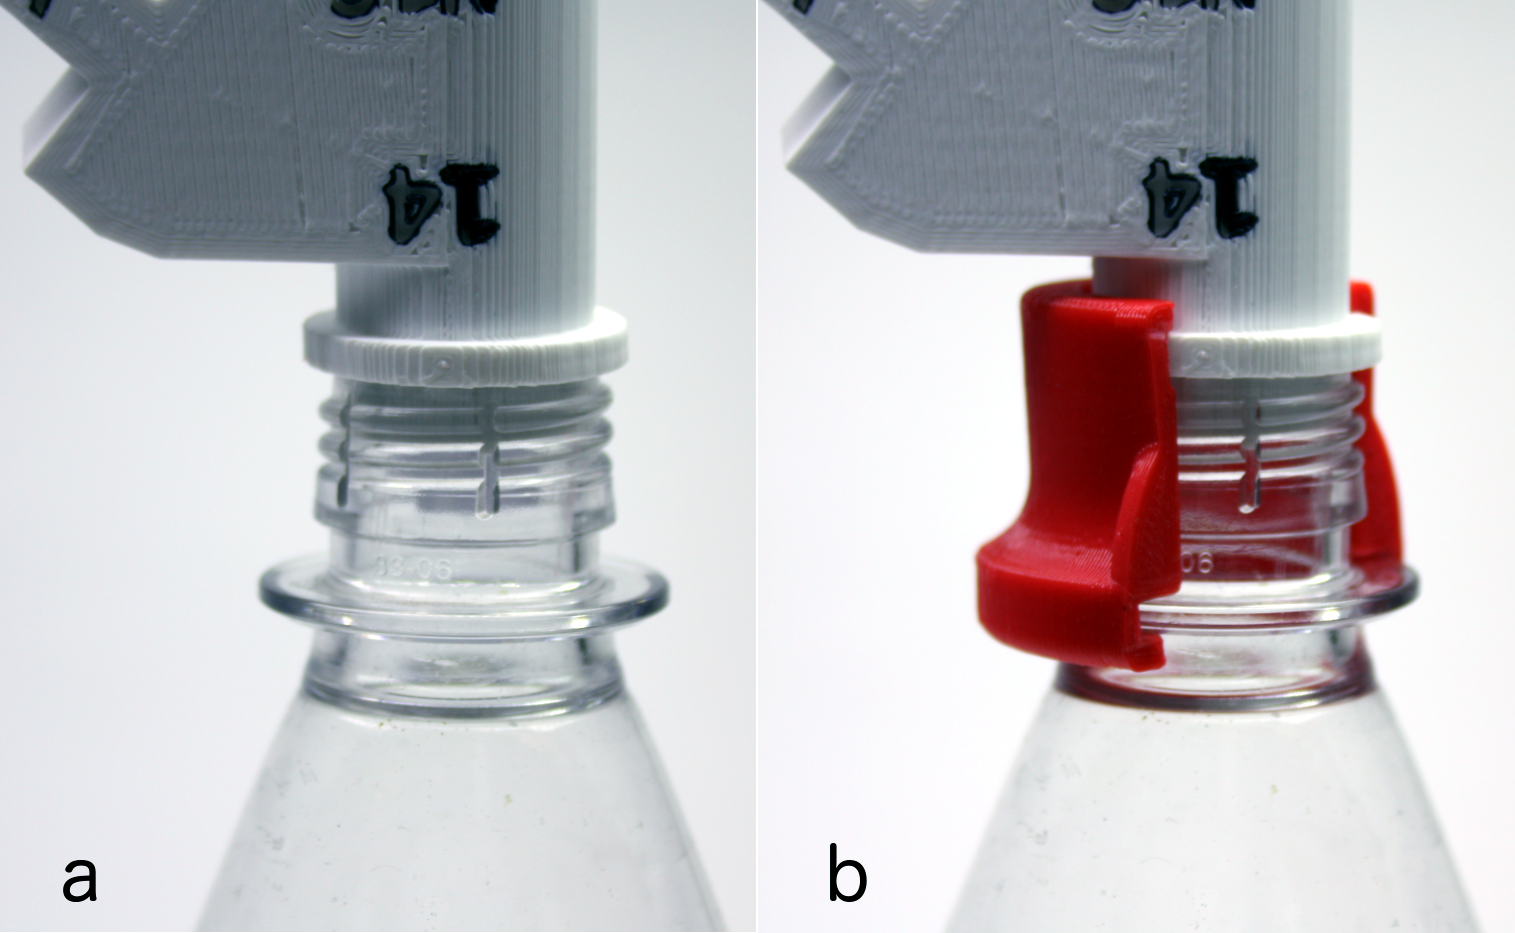
\includegraphics[width=\textwidth]{Hardware/connectors.png}
    \caption{(a) The connector is inserted into the bottle opening and (b) secured with a cuff.}
    \centering
    \label{fig:connector}
\end{figure}

\subsection{Hinging Hubs}\label{sec:hinges}
In order to introduce movement to truss structures, we came across some challenges. Multiple links have to be able to pivot around a common center. This kind of spherical motion can potentially be achieved using ball joints, however these joints typically only allow for a connection of two links without causing obstruction.\\
We solve this issue by using a \textit{spherical joint mechanism} \cite{sofla:2009, spinos2:2017}. As can be seen in Figure \ref{fig:hinge_chain}, these chains of hinges can connect multiple links, which can all rotate around the same center. This is possible, because the axes of rotation do not occupy the rotational center itself, creating room for movement.\\
\begin{figure}[ht!]
    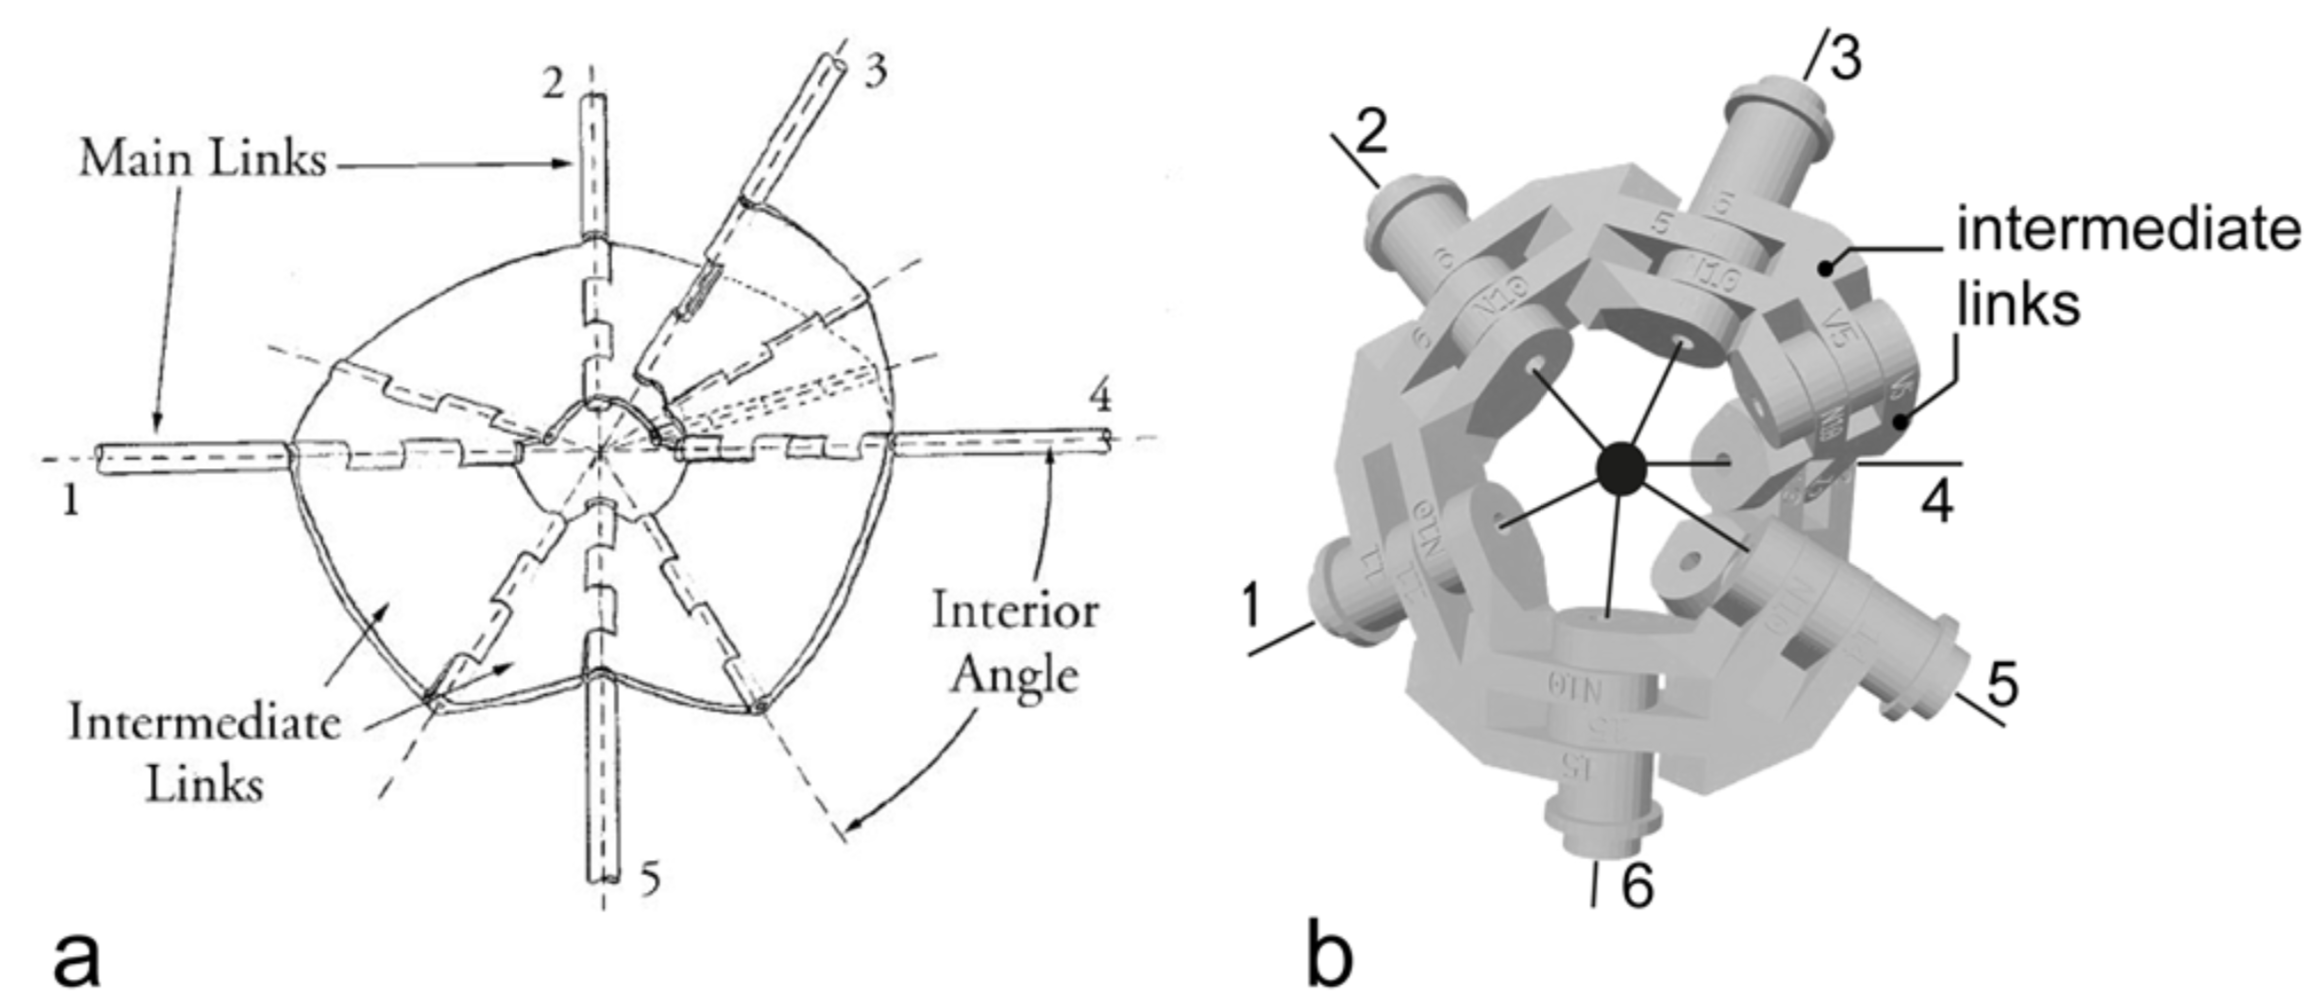
\includegraphics[width=\textwidth]{Hardware/hinge_chain.png}
    \centering
    \caption{(a) spherical joint mechanism connecting 5 links. (b) rendering of TrussFormers' hinge chain design connecting 6 links.}
    \label{fig:hinge_chain}
\end{figure}
We started out using an open hinge chain, meaning that the chain had special end parts which were only connected on one side. This gave us a lot of freedom of movement, however it turned out that this design was not strong enough for our needs and frequently broke during testing builds of the T-Rex. This required us to rethink our design and we came up with a closed hinge chain design.\\
The degrees of freedom our hinge system needs to have, underly constraints, allowing us to limit the possible movement of the hinges. The original spherical joint mechanism shown in Figure \ref{fig:hinge_chain}a connected all edges using two hinges, allowing for 2 DoF. This is not necessary if we are dealing with truss structures. An example of TrussFormers's hinge design can be seen in Figure \ref{fig:hinge_chain}b. Only edge 4 is connected to its neighboring edges using two intermediate hinges. All other edges only require rotation (resulting in 1 DoF).\\
The hinge chains are arranged automatically in the structure by our TrussFormer system. This heuristic approach will be described in more detail in Section \ref{sec:hinge_placement_impl}.

\subsubsection{3D printing}
The hubs and connecting cuffs are printed using consumer-grade desktop \ac{FDM} 3D printers. The filament consists of \ac{PLA} plastic and the printed objects have a 15\% infill with a wall thickness of 3 mm. We chose PLA filament instead of \ac{ABS} primarily because it is easier to handle. ABS plastic, while being stronger, needs to be printed on a heated surface, which not many mid-range printers have. As we designed the TrussFormer system for 3D-printing enthusiasts and not professionals, we wanted to target owners of consumer-grade printers. Additionally, PLA consists of organic materials (mainly cornstarch and sugarcane), which makes it biodegradable, as opposed to ABS plastic, which is oil-based.\\
A hub consumes about 50-150g of filament, resulting in a cost of 1-3€.

\section{Actuation}
\begin{figure}[ht!]
    \includegraphics[width=\textwidth]{Hardware/hardware_setup.png}
    \centering
    \caption{Hardware setup for controlling the T-Rex, with Arduino, electric pressure control valves, and compressor.}
    \label{fig:hardware_setup}
\end{figure}
Figure \ref{fig:hardware_setup} shows the main parts of our hardware setup. The electrically controllable pressure regulators receive signals from the control board and limit the air pressure according to the needed level of extension of a given actuator. One pressure regulator is connected to exactly on actuator. The \textit{Airpress HL 360} compressor delivers the regulators with up to 8 bars of pressure.\\
The limited pressure is tunneled to a valve terminal. This terminal opens and closes airflow to the actuators. If it opens a valve, the regulated pressure will enter its air circuit and change the extension of the actuator. If it closes it, the pressure will stay constant and the actuator keeps its position.

\subsection{Electric Actuators}
Early TrussFormer prototypes used electric actuators, instead of the pneumatic ones we used for the T-Rex. Electric actuators can produce a fairly large force and are easier to control, as they can usually provide their current extension. However, at around 0.03 m/s they extend very slowly, compared to our pneumatic actuators, which can reach more than 2 m/s. As our structures are fairly lightweight, the force of the actuators is not a big concern, while the higher speed of pneumatic actuators enables us to create more dynamic structures.

\subsection{Pneumatic Actuators}
We use different kinds of pneumatic actuators, depending on the force needed. Our actuators usually have a piston diameter of 20 - 35 mm and can extend from 40 cm to 80 cm. This length works well with our bottle links, which are 60 cm long, meaning that the middle position of the actuator makes it the same length as the links.\\
A common actuator that could be used is the Festo DSNU round cylinder with a diameter of 32 mm and a hub of 30 cm, as shown in Figure \ref{fig:festo_cylinder}. This cylinder can operate with up to 10 bars, the following values were measured with 6 bars of pressure and at room temperature. Under these circumstances, this actuator can achieve an extension rate of up to 2.3 m/s (without load) with a force of 480N on the extending stroke and 415N on retraction. This force is sufficient for moving the head of our T-Rex up and down, which is the motion requiring the most force in our design. For higher loads, e.g. lifting a human, an actuator with a bigger diameter should be used. A Festo actuator with a diameter of 50 mm is capable of achieving up to 1200 N of force on the extending stroke at 6 bars.
\begin{figure}[ht!]
    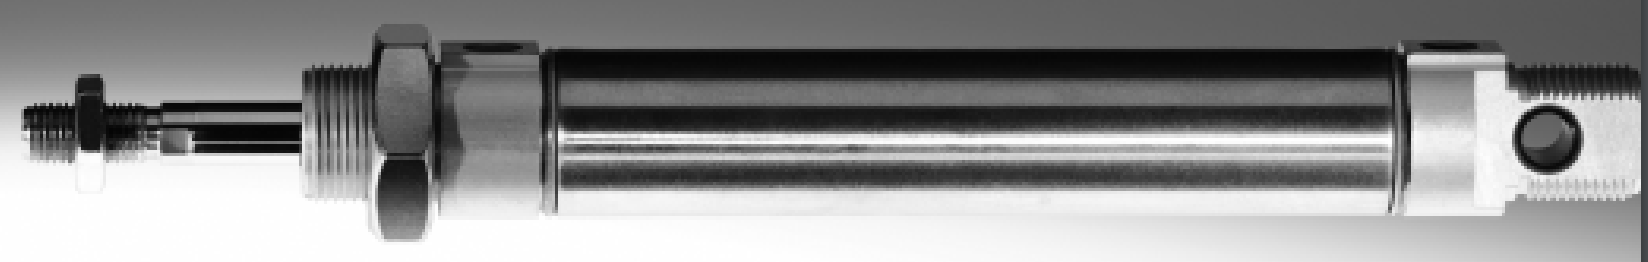
\includegraphics[width=\textwidth]{Hardware/festo_cylinder.png}
    \centering
    \caption{A Festo DSNU cylinder with 32 mm cylinder diameter and 30 cm of hub, as used in our T-Rex.}
    \label{fig:festo_cylinder}
\end{figure}

\section{Control System}
We control the pneumatic actuators using a MIDI control interface. The slider inputs are sent to an Arduino which translates them to control signals for digitally controllable pressure valves. The actuators have two connections for air pipes: one for extending the actuator and one for retracting it. The signal from the slider is interpreted as a mixture between these two inputs, with the slider at the top meaning that all the air is send to the extending input and the slider at the bottom completely retracting it.

\subsection{Valves}
We used two different kinds of valves. \textit{Proportional pressure regulators}, such as the Festo VPPM (Figure \ref{fig:valves} (left)), are used for open-loop pressure control. Communication to these regulators is achieved with an IO link, which can be connected to a control unit. Digital signals are translated to a proportional opening of the valves, providing a constant and reliable pressure. VPPMs have one input and one output valve. This fact differentiates proportional pressure regulators from \textit{proportional directional control valves}, like the Festo MPYE (Figure \ref{fig:valves} (right)). These valves have one input, but two outputs, making it possible to connect it to both inputs of a pneumatic actuator. Controlling these valves works similar to proportional pressure regulators and also uses a simple IO link. Digital signals send to this type of valve do not, however, only control the pressure of these outputs, but also the ratio between these two outputs. This makes positional control of actuators possible.

\begin{figure}[ht!]
    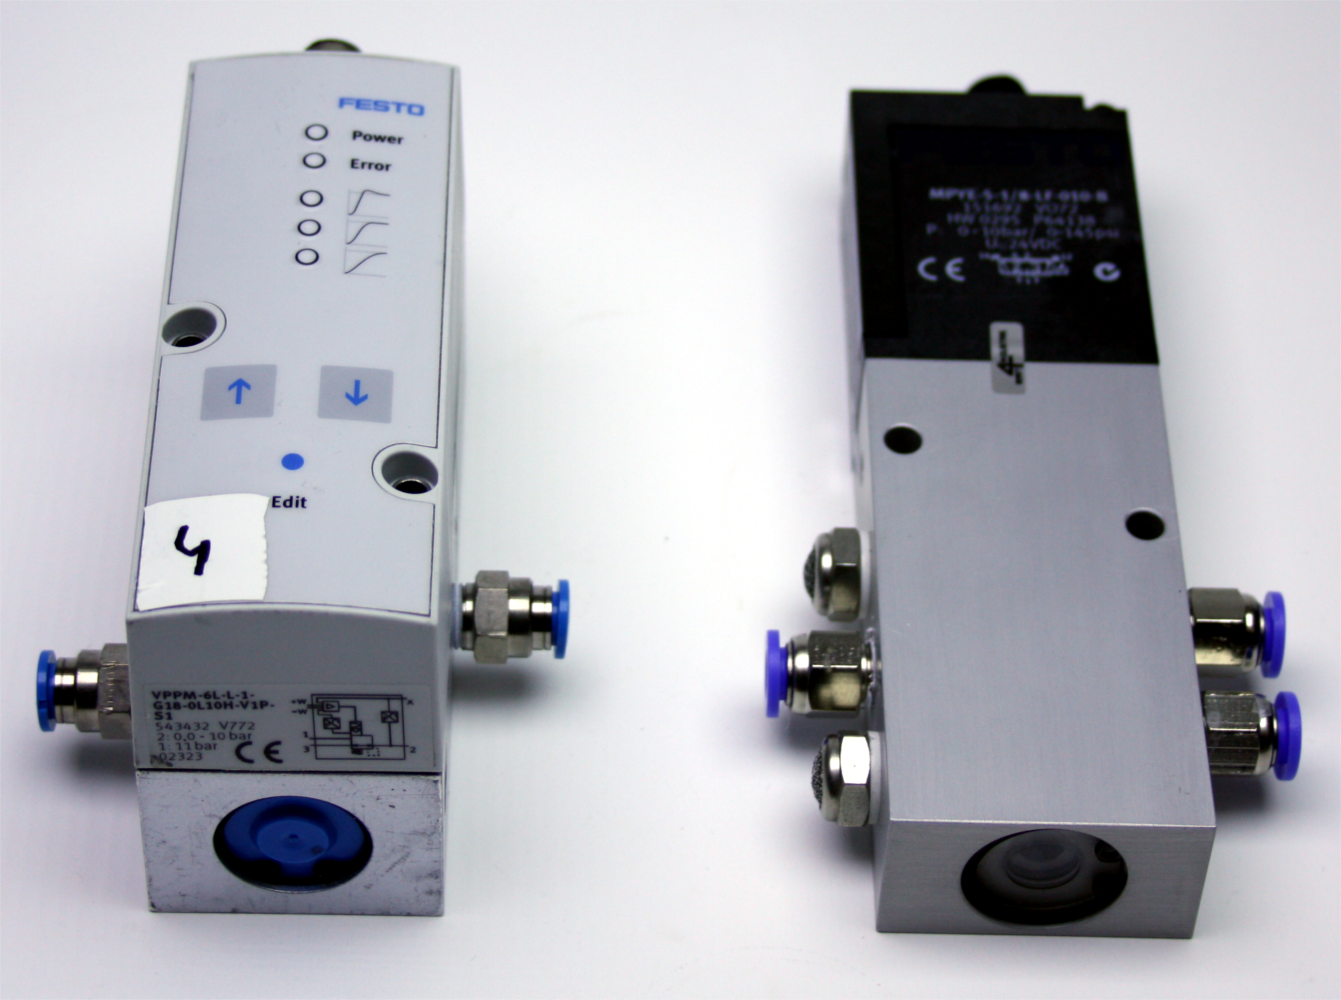
\includegraphics[width=\textwidth]{Hardware/valves.png}
    \centering
    \caption{(left) A proportional pressure regulator with one input and one output. (right) A proportional directional control valve, with one input and two outputs. Both can be attached to an IO link on the top.}
    \label{fig:valves}
\end{figure}

\subsection{Position Sensing}
The MIDI controller is a well working possibility to control actuators. It is, however, an open-loop control, meaning it can not react to external influences, like weight shifts or additional pressure acting on edges. This is not a big problem for our T-Rex example, as it usually moves undisturbed and without external interaction. If we want to create an interactive object, this will not be sufficient.\\
Pneumatic actuators on their own tend to not have the possibility to measure their own rate of extension. We therefore created an easy to build distance sensor, using a string on a spindle. One side of the string is attached to the piston part of the actuator, while the spindle is attached to the static body. While the actuator extends, the spindle will spin, releasing more string. We attached a rotary encoder to the spindle, counting its rotations. Using the diameter of the reel, we can calculate how much string was released during the extension, which correlates to the extension of the piston itself. A prototype of this method can be seen in Figure \ref{fig:position_control}.\\
\begin{figure}[ht!]
    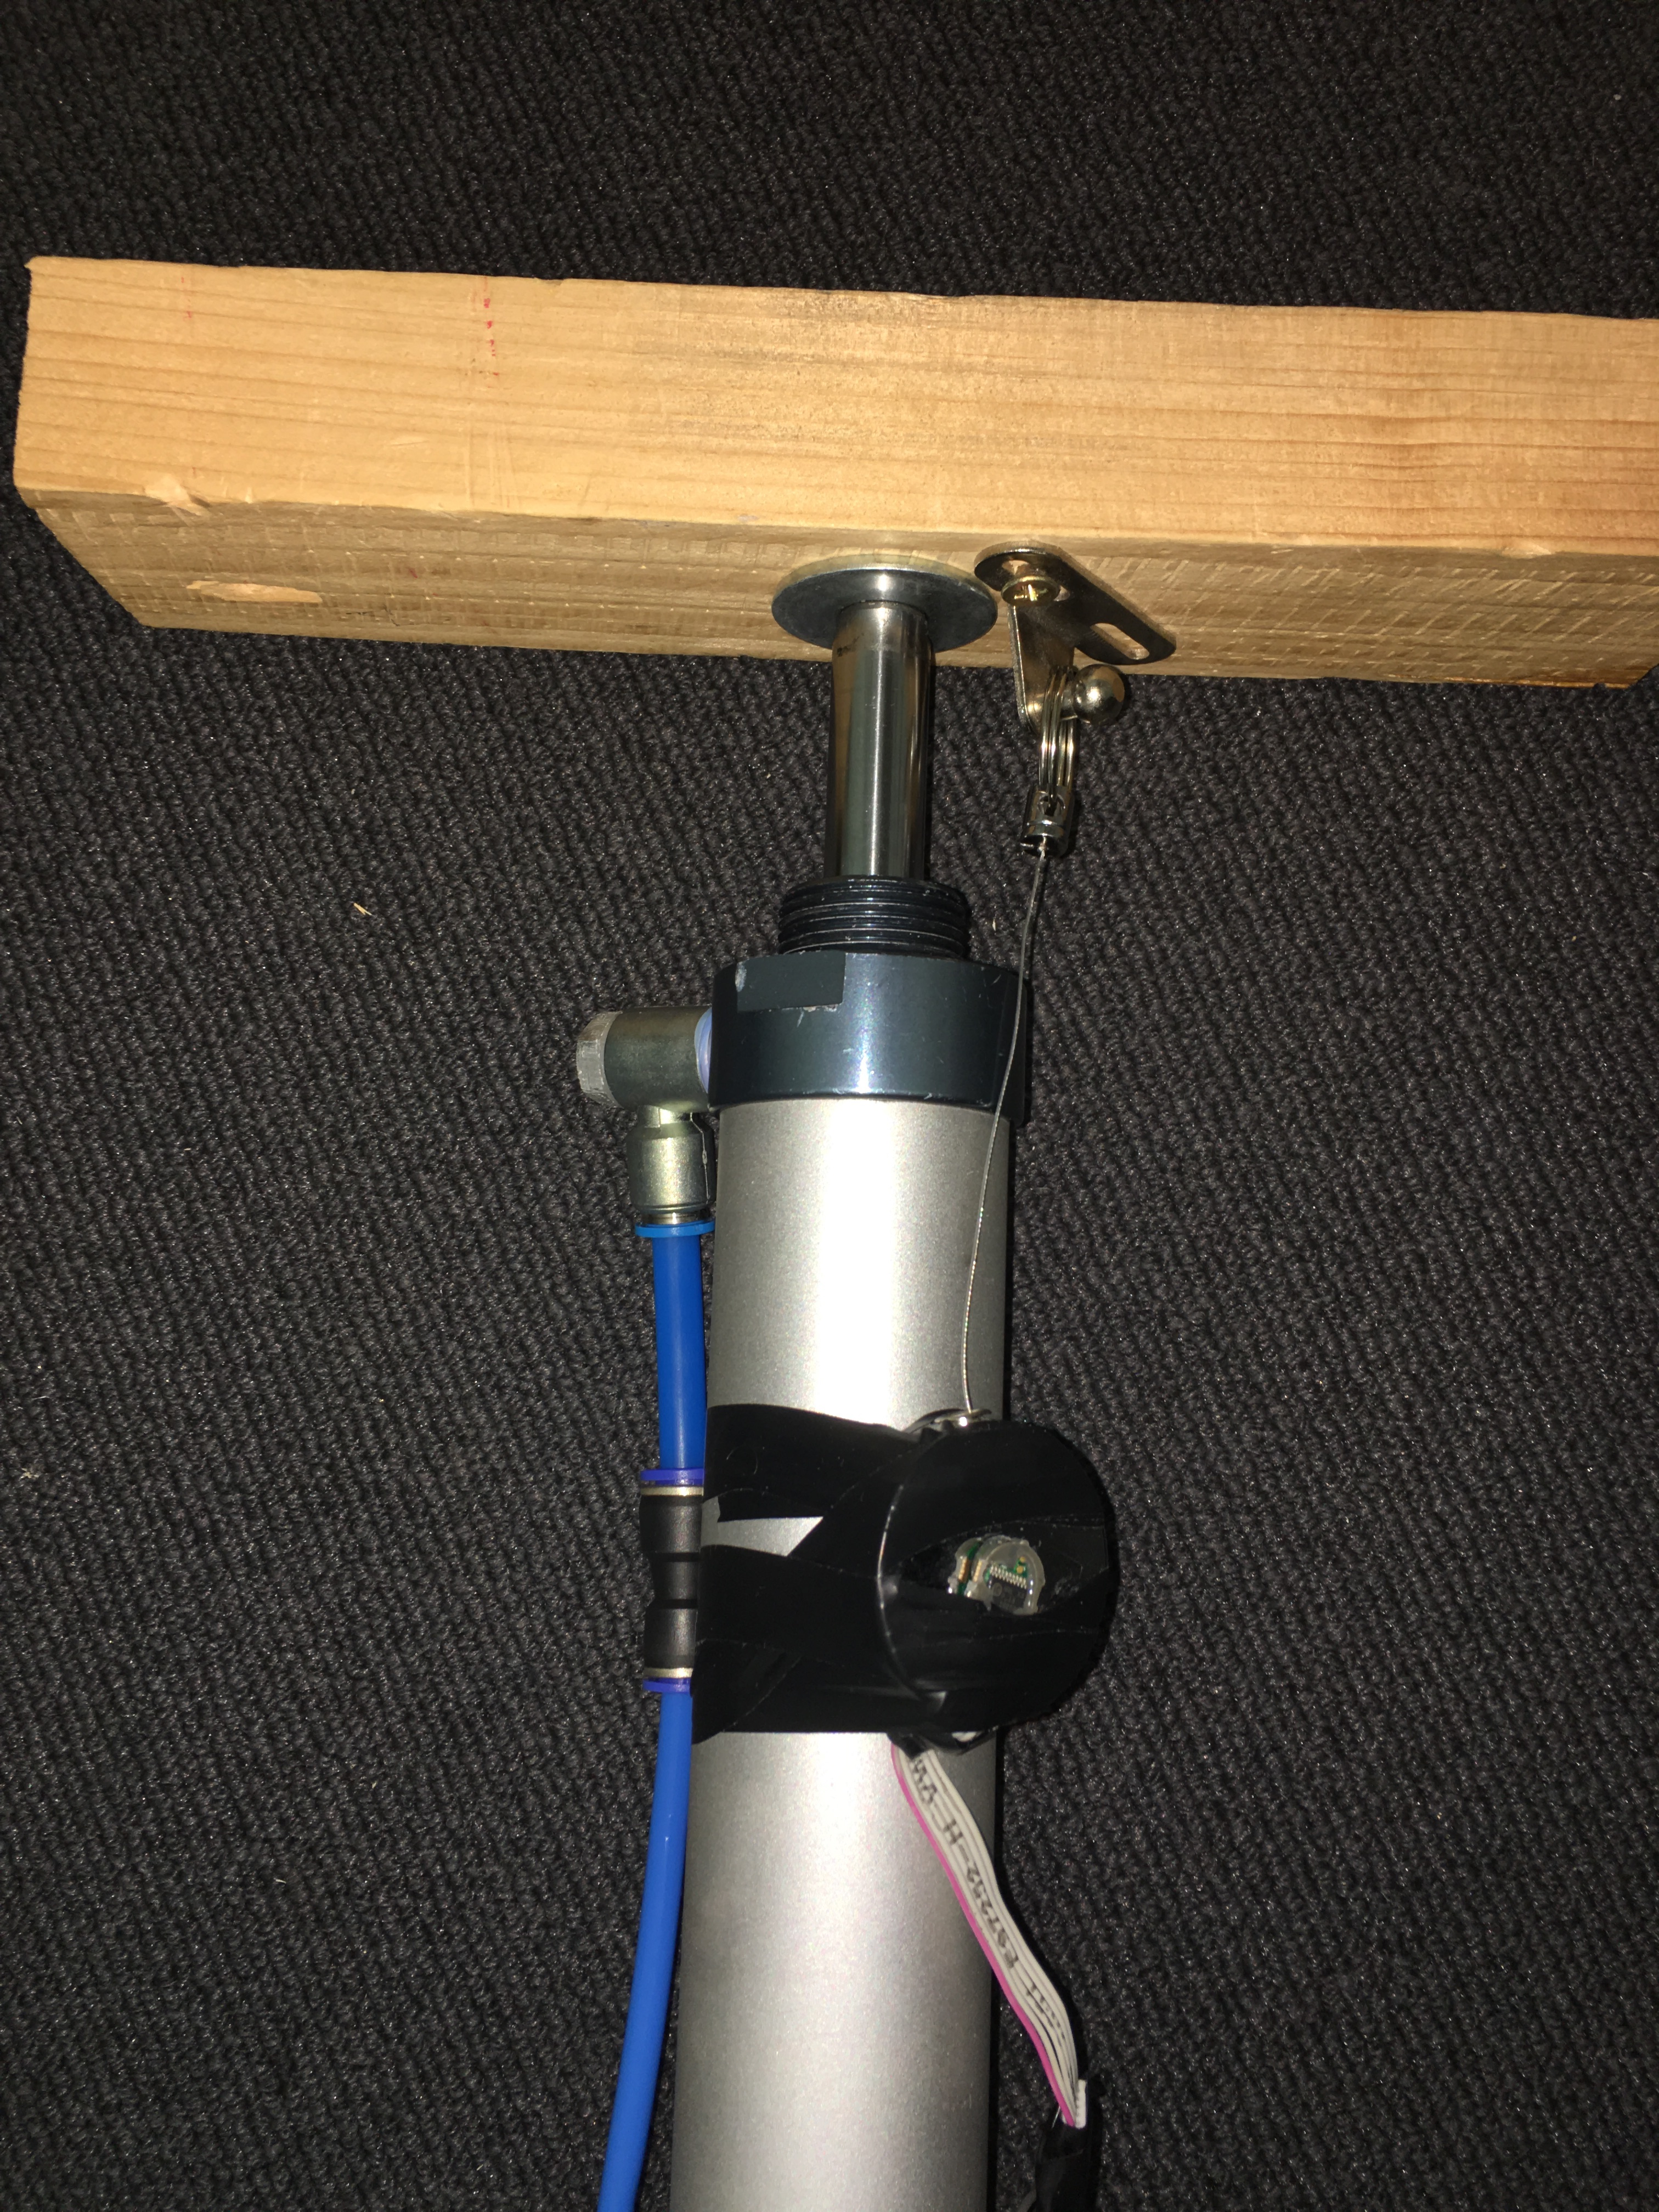
\includegraphics[width=\textwidth]{Hardware/position_controller.png}
    \centering
    \caption{We use a badge holder with a rotary encoder for position sensing. The string of the holder is attached to the actuators body and the extending piston. On extension, the string will roll off the spindle, which we can measure with the encoder and translate into a length.}
    \label{fig:position_control}
\end{figure}
Using this approach, we can have closed-loop control of the actuators, making it possible to constantly monitor its extension and apply force accordingly.

\subsubsection{PID Controller}
We created a rudimentary motion-platform using closed-loop PID control (s.a. Section \ref{sec:pid}). The motion platform has three modes. It starts fully extended, applying a little bit of pressure to keep the actuator upright, but little enough that a human sitting on it pushed it back. If the actuator reached an extension of 10 cm, the control loop applied a holding force, making it possible to sit on the platform without it moving. If the person on the platform applied more force, pushing the piston further down, the third mode activated, which made it oscillate up and down.

\subsection{Control Units}
For our control module we have different approaches for open and closed loop control, as well. Open loop control can be achieved with a simple \textit{Arduino}. It can be attached to a control interface, such as our MIDI controller, and translate the given inputs into signals for the valves.\\
Another logic controller we used is the \textit{Controllino}.
 % 5-10 pages
\cleardoublepage\chapter{Implementation}\label{ch:implementation}
We implemented \trussFabName{} as a plug-in for the 3D modeling software \textit{SketchUp}. It is primarily written in Ruby and JavaScript.\unsure{Do we assume TrussFormer is a new product, which uses similar functionality as TrussFab, or do we say it is an improvement?}

\section{Architecture}
The software can be divided into four components. The most user-facing one is the designer. The other components handle the physics simulation of the created structures, minimization logic for the created hubs and hinges and the 3D print export.\\
\\
\subsection{Designer}
All components are stored in a graph structure. The building parts are \textit{Edges}, \textit{Nodes} and \textit{Triangles}. They all inherit \textit{GraphObject}. The purpose of these objects is providing user-facing functionalities and storing lower-level components. An overview of the graph structure can be seen in \ref{fig:graph}.\\
The \textit{Graph} is implemented as a Singleton \improvement{explain what a Singleton is} that stores and provides access to all GraphObjects, creates new ones and provides convenience functions for user interactions, such as finding the node closest to the mouse cursor. As this class is a singleton, every module of the software has access to the objects. Each SketchUp object has access to its underlying logic-bearing component, called \textit{SketchupObject}.\improvement{Clarify. Either explain what that means (Hubs, Links, Surfaces) or at least have a forward reference} The access to this functionality is, however, not implemented in this superclass, but in each subclass, having the specific name. This design decision was made to improve code readability and coding errors by accessing the wrong SketchupObject.\improvement{Show before and after code snippet}\\
\begin{figure}
    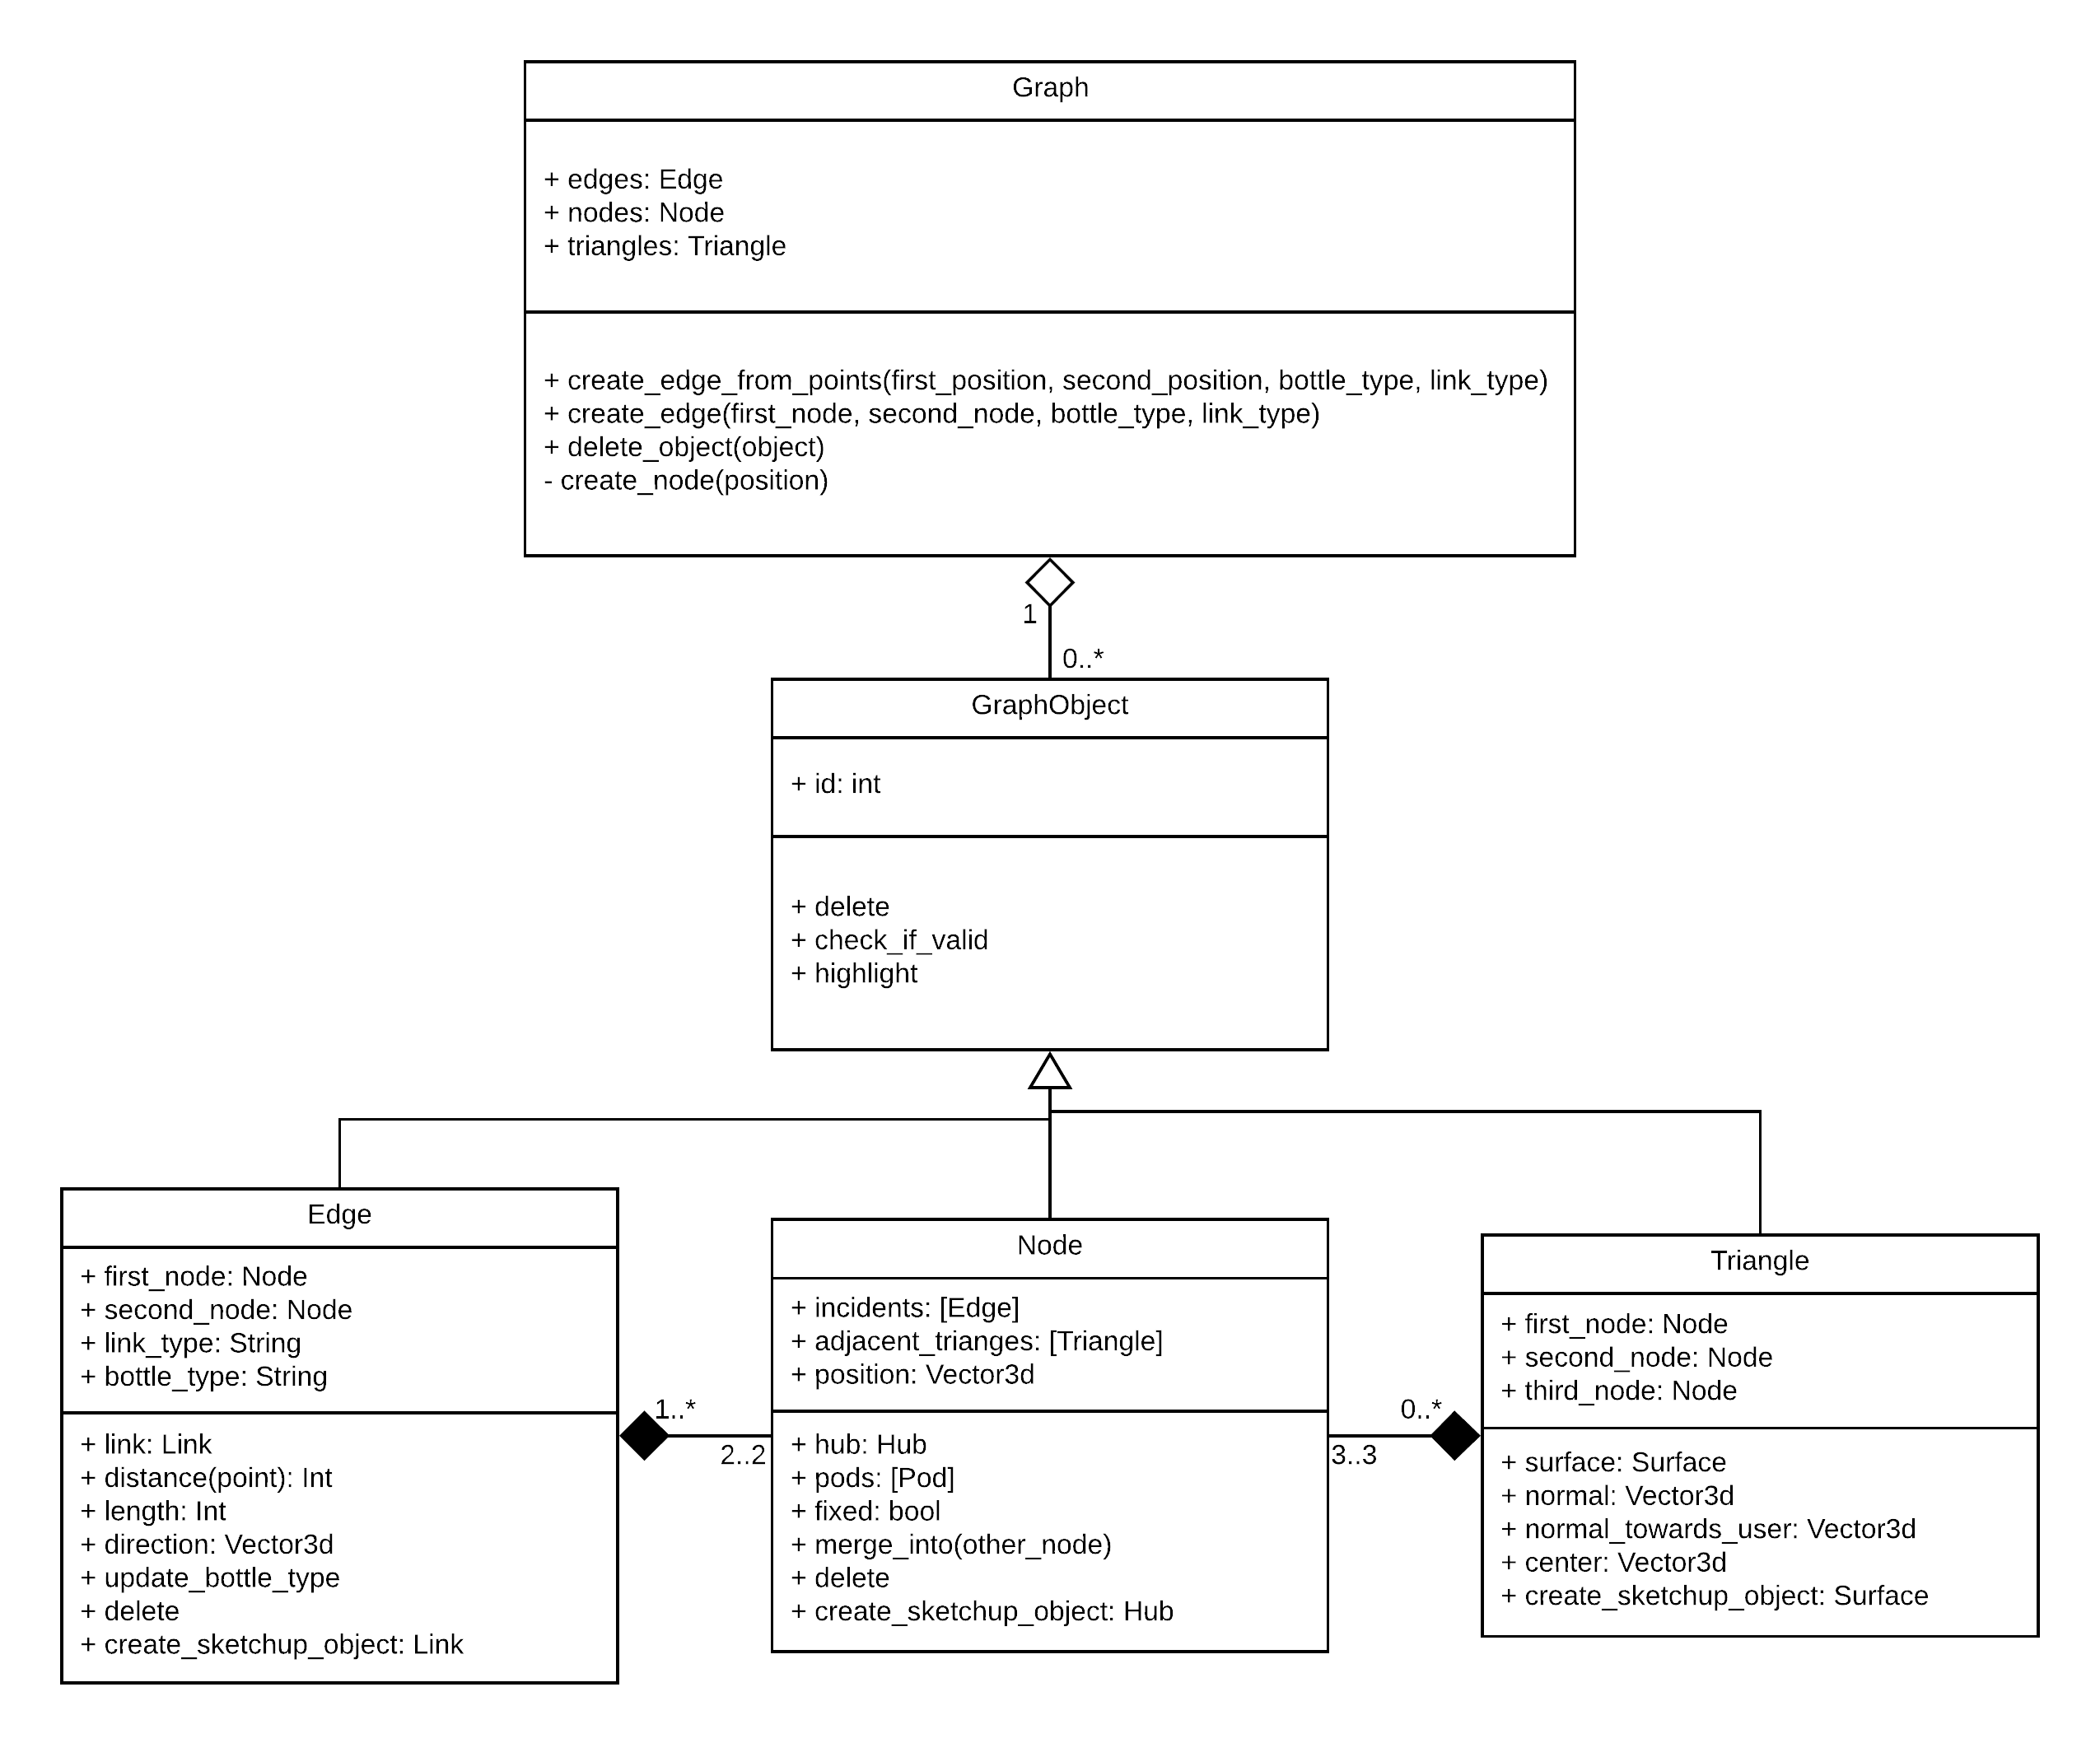
\includegraphics[width=\textwidth]{implementation/TrussFab_Graph.png}
    \centering
    \caption{Class Diagram showing the high-level Graph Structure of the TrussFab Designer}
    \label{fig:graph}
\end{figure}
The responsibility of the GraphObject class is primarily unifying the way the appearance in SketchUp of the underlying object can be changed as much as possible. This includes highlighting a specific object if the mouse hovers over it, resetting the object to its default state and creating and deleting it. More complex methods need to be implemented in the respective subclass.\\
\textit{Nodes} are the connecting components of the structure. \textit{Edges}, as well as \textit{Triangles} are created based on Nodes. Apart from storing adjacent Edges and Triangles, a Node can specify their positions in the SketchUp world. The Nodes' adjacent objects constantly check if their position has changed and update their SketchUp representation accordingly. If the structure is deformed in such a way that a Node will be at the same position as another one, the Node object can automatically merge into the other Node. The Node will iterate over all its adjacent Edges and tell each one, apart from the Edges that run from the other Node to the Edge the Node is hinging around (i.e. the Edge that is opposite the Node), to exchange itself with the Node it wants to merge into. These Edges are removed from its own adjacent Edges and added to the collection of the new Node. The same happens for all adjacent Triangles. As a last step, the Node deletes itself and all remaining adjacent Edges and Triangles (which will be the Edges and Triangles that got merged). The object will then be adapted according to the new positions using the \textit{Relaxation algorithm}, described in section \ref{relaxation}.\\
\clearpage
\begin{lstlisting}[language=Ruby, caption=Merging of two Nodes]
  def merge_into(other_node)
    merged_incidents = []
    @incidents.each do |edge|
      edge_opposite_node = edge.opposite(self)
      next if other_node.edge_to?(edge_opposite_node)
      edge.exchange_node(self, other_node)
      other_node.add_incident(edge)
      merged_incidents << edge
    end
    @incidents -= merged_incidents

    merged_adjacent_triangles = []
    @adjacent_triangles.each do |triangle|
      new_triangle = triangle.nodes - [self] + [other_node]
      next unless Graph.instance.find_triangle(new_triangle).nil?
      triangle.exchange_node(self, other_node)
      other_node.add_adjacent_triangle(triangle)
      merged_adjacent_triangles << triangle
    end
    @adjacent_triangles -= merged_adjacent_triangles

    delete
  end
\end{lstlisting}\label{merging_code}
Another component that is tightly coupled to Nodes are \textit{Pods}. A Pod acts as a stand for the object and tells TrussFab that this Node should not change its position.\todo{add image}
\\- tight coupling to SketchUp (uses SketchUp Elements, SketchUp rendering engine, ...)\unsure{Maybe the details should be subsections?}\\
\subsection{Physics Simulation}
- Based on \textit{MSPhysics} by Anton Synytsia
- Ruby wrapper around C++ physics engine \textit{Newton Dynamics}
- Implemented as a \textit{SketchUp Animation}
- implements \textit{nextFrame} method
- this method is called every time SketchUp has finished rendering a frame
- this method does:
\begin{enumerate}
    \item tell Sketchup to render new frame (SketchUp will render the positions calculated in the previous world update: make use of calculate new update while sketchup already renders new positions)
    \item call \textit{update\_world}, which does, world\_iterations times:
    \begin{itemize}
        \item update forces, i.e. call apply predetermined forces (e.g. weights on hubs, calculations of PID controller)
        \item call \textit{world.advance}: Tell MSPhysics, that a new world update is available and let it calculate new forces after positional updates
        \item record tensions on links, for visualization later. This has to be recorded, because for each render step, a number of world updates are done. We don't want to miss crucial force updates
        \item visualize forces: send color information to SketchUp, indicating the strength of the tension on links
    \end{itemize}
    \item update entity positions: tell SketchUp where components have to be rendered next time
    \item send data to ui: send sensor data to ui charts, if needed
\end{enumerate}
\subsection{Minimization Logic}
- elongates and shortens edges so that maximum movement is possible with minimum material use\\
- uses iterative relaxation algorithm, will be explained in \ref{relaxation}

\subsection{Export}

\section{TrussFab Designer}
The TrussFab Designer provides static sketching functionalities. It can create and display different predefined models, has knowledge about the connections of different components and can modify the resulting objects structure.

\subsection{User Interface}

\subsection{Structure Creation}
Terminology:\\
\begin{enumerate}
    \item Edge:
    \begin{enumerate}
        \item Connects two nodes
        \item Can be:
        \begin{enumerate}
            \item Bottle Link
            \item Actuator
            \item PID link
        \end{enumerate}
    \end{enumerate}
\end{enumerate}

\subsection{Modifying the Structure}

\subsection{Relaxation Algorithm}\label{relaxation}

\subsection{OpenSCAD Export}\label{sec:openscad_impl}

\section{TrussFormer Physics Engine}

\subsection{Simulation}
- only hubs are simulated to improve performance

\subsection{Automatic Actuator Placement (if it works soon-ish)}

\section{Force Control}

\subsection{PID}
 % 25-30 pages This is what the Zweitkorrektor probably will focus on. Make it count!
\cleardoublepage\chapter{Conclusion}\label{ch:conclusion}
We created a system that enables users to design and fabricate large-scale dynamic truss structures. Our system consists of an editor, which supports creating and simulating stable truss objects with the help of a physics engine. Users can simulate motion by placing linear actuators in the structure and observe occurring forces by interactively moving the structure. Motion patterns can be created by using the keyframe animation feature. This way, the complicated motion distribution in the trusses can be thoroughly tested before building the object.\\
Our export feature enables users to generate .stl files, based on the designed object, which can be 3D printed and assembled. The animation is stored in an Arduino-readable format, so the designed object can be completely recreated in the real world.\\
For assembly, users connect PET bottles to the 3D printed hubs. An ID system clarifies which of these hubs belong together.

\section{Closed-loop Positional Control}
We already made first advances towards integrating closed-loop actuator control into our system.
 % 2-4 pages

% ********************************************************************
% Backmatter
%*******************************************************
% If you want to have an appendix uncomment the lines below
%\appendix
%\renewcommand{\thechapter}{\alph{chapter}}
%\cleardoublepage
% %********************************************************************
% Appendix
%*******************************************************
% If problems with the headers: get headings in appendix etc. right
%\markboth{\spacedlowsmallcaps{Appendix}}{\spacedlowsmallcaps{Appendix}}
\chapter{Appendix Test}
Lorem ipsum at nusquam appellantur his, ut eos erant homero
concludaturque. Albucius appellantur deterruisset id eam, vivendum
partiendo dissentiet ei ius. Vis melius facilisis ea, sea id convenire
referrentur, takimata adolescens ex duo. Ei harum argumentum per. Eam
vidit exerci appetere ad, ut vel zzril intellegam interpretaris.
\graffito{More dummy text.}

%Errem omnium ea per, pro congue populo ornatus cu, ex qui dicant
%nemore melius. No pri diam iriure euismod. Graecis eleifend
%appellantur quo id. Id corpora inimicus nam, facer nonummy ne pro,
%kasd repudiandae ei mei. Mea menandri mediocrem dissentiet cu, ex
%nominati imperdiet nec, sea odio duis vocent ei. Tempor everti
%appareat cu ius, ridens audiam an qui, aliquid admodum conceptam ne
%qui. Vis ea melius nostrum, mel alienum euripidis eu.

\section{Appendix Section Test}
Test: \autoref{tab:moreexample} (This reference should have a
lowercase, small caps \spacedlowsmallcaps{A} if the option
\texttt{floatperchapter} is activated, just as in the table itself
 $\rightarrow$ however, this does not work at the moment.)

\begin{table}[h]
    \myfloatalign
    \begin{tabularx}{\textwidth}{Xll} \toprule
        \tableheadline{labitur bonorum pri no} & \tableheadline{que vista}
        & \tableheadline{human} \\ \midrule
        fastidii ea ius & germano &  demonstratea \\
        suscipit instructior & titulo & personas \\
        %postulant quo & westeuropee & sanctificatec \\
        \midrule
        quaestio philosophia & facto & demonstrated \\
        %autem vulputate ex & parola & romanic \\
        %usu mucius iisque & studio & sanctificatef \\
        \bottomrule
    \end{tabularx}
    \caption[Autem usu id]{Autem usu id.}
    \label{tab:moreexample}
\end{table}

%Nulla fastidii ea ius, exerci suscipit instructior te nam, in ullum
%postulant quo. Congue quaestio philosophia his at, sea odio autem
%vulputate ex. Cu usu mucius iisque voluptua. Sit maiorum propriae at,
%ea cum primis intellegat. Hinc cotidieque reprehendunt eu nec. Autem
%timeam deleniti usu id, in nec nibh altera.




\section{Another Appendix Section Test}
Equidem detraxit cu nam, vix eu delenit periculis. Eos ut vero
constituto, no vidit propriae complectitur sea. Diceret nonummy in
has, no qui eligendi recteque consetetur. Mel eu dictas suscipiantur,
et sed placerat oporteat. At ipsum electram mei, ad aeque atomorum
mea. There is also a useless Pascal listing below: \autoref{lst:useless}.

\begin{lstlisting}[float=b,language=Pascal,frame=tb,caption={A floating example (\texttt{listings} manual)},label=lst:useless]
for i:=maxint downto 0 do
begin
{ do nothing }
end;
\end{lstlisting}

%Ei solet nemore consectetuer nam. Ad eam porro impetus, te choro omnes
%evertitur mel. Molestie conclusionemque vel at, no qui omittam
%expetenda efficiendi. Eu quo nobis offendit, verterem scriptorem ne
%vix.



%********************************************************************
% Other Stuff in the Back
%*******************************************************
\cleardoublepage%********************************************************************
% Bibliography
%*******************************************************
% work-around to have small caps also here in the headline
% https://tex.stackexchange.com/questions/188126/wrong-header-in-bibliography-classicthesis
% Thanks to Enrico Gregorio
\defbibheading{bibintoc}[\bibname]{%
  \phantomsection
  \manualmark
  \markboth{\spacedlowsmallcaps{#1}}{\spacedlowsmallcaps{#1}}%
  \addtocontents{toc}{\protect\vspace{\beforebibskip}}%
  \addcontentsline{toc}{chapter}{\tocEntry{#1}}%
  \chapter*{#1}%
}
\printbibliography[heading=bibintoc]

% Old version, will be removed later
% work-around to have small caps also here in the headline
%\manualmark
%\markboth{\spacedlowsmallcaps{\bibname}}{\spacedlowsmallcaps{\bibname}} % work-around to have small caps also
%\phantomsection
%\refstepcounter{dummy}
%\addtocontents{toc}{\protect\vspace{\beforebibskip}} % to have the bib a bit from the rest in the toc
%\addcontentsline{toc}{chapter}{\tocEntry{\bibname}}
%\label{app:bibliography}
%\printbibliography

\cleardoublepage%*******************************************************
% Declaration
%*******************************************************
\refstepcounter{dummy}
\pdfbookmark[0]{Declaration}{declaration}
\chapter*{Declaration}
\thispagestyle{empty}
I certify that the material contained in this thesis is my own work and does not
contain unreferenced or unacknowledged material. I also warrant that the above
statement applies to the implementation of the project.

\bigskip

\setlength{\parindent}{0pt}
Hiermit versichere ich, dass ich die vorliegende Arbeit selbstständig verfasst
und keine anderen als die angegebenen Hilfsmittel verwendet habe. Ich erkläre
hiermit weiterhin die Gültigkeit dieser Aussage für die Implementierung des
Projekts.

\bigskip
 
\noindent\textit{\myLocation, \myTime}

\smallskip

\begin{flushright}
    \begin{tabular}{m{5cm}}
        \\ \hline
        \centering\myName \\
    \end{tabular}
\end{flushright}

% \cleardoublepage\pagestyle{empty}

\hfill

\vfill


\pdfbookmark[0]{Colophon}{colophon}
\section*{Colophon}
This document was typeset using the typographical look-and-feel \texttt{classicthesis} developed by Andr\'e Miede and Ivo Pletikosić.
The style was inspired by Robert Bringhurst's seminal book on typography ``\emph{The Elements of Typographic Style}''.
\texttt{classicthesis} is available for both \LaTeX\ and \mLyX:
\begin{center}
\url{https://bitbucket.org/amiede/classicthesis/}
\end{center}
Happy users of \texttt{classicthesis} usually send a real postcard to the author, a collection of postcards received so far is featured here:
\begin{center}
\url{http://postcards.miede.de/}
\end{center}
Thank you very much for your feedback and contribution.

\bigskip

\noindent\finalVersionString

%Hermann Zapf's \emph{Palatino} and \emph{Euler} type faces (Type~1 PostScript fonts \emph{URW
%Palladio L} and \emph{FPL}) are used. The ``typewriter'' text is typeset in \emph{Bera Mono},
%originally developed by Bitstream, Inc. as ``Bitstream Vera''. (Type~1 PostScript fonts were made
%available by Malte Rosenau and
%Ulrich Dirr.)

%\paragraph{note:} The custom size of the textblock was calculated
%using the directions given by Mr. Bringhurst (pages 26--29 and
%175/176). 10~pt Palatino needs  133.21~pt for the string
%``abcdefghijklmnopqrstuvwxyz''. This yields a good line length between
%24--26~pc (288--312~pt). Using a ``\emph{double square textblock}''
%with a 1:2 ratio this results in a textblock of 312:624~pt (which
%includes the headline in this design). A good alternative would be the
%``\emph{golden section textblock}'' with a ratio of 1:1.62, here
%312:505.44~pt. For comparison, \texttt{DIV9} of the \texttt{typearea}
%package results in a line length of 389~pt (32.4~pc), which is by far
%too long. However, this information will only be of interest for
%hardcore pseudo-typographers like me.%
%
%To make your own calculations, use the following commands and look up
%the corresponding lengths in the book:
%\begin{verbatim}
%    \settowidth{\abcd}{abcdefghijklmnopqrstuvwxyz}
%    \the\abcd\ % prints the value of the length
%\end{verbatim}
%Please see the file \texttt{classicthesis.sty} for some precalculated
%values for Palatino and Minion.
%
%    \settowidth{\abcd}{abcdefghijklmnopqrstuvwxyz}
%    \the\abcd\ % prints the value of the length


\end{document}
% ********************************************************************
